\documentclass[12pt,a4paper]{scrartcl}

\usepackage[utf8]{inputenc}
\usepackage[T1]{fontenc}
\usepackage[british,UKenglish,USenglish,american]{babel}

\usepackage{bbm}
\usepackage{hyperref}
\usepackage[pdftex]{graphicx}
\usepackage{graphicx}
\usepackage{subcaption}
\usepackage{latexsym}
\usepackage{amsmath,amssymb,amsthm}
\allowdisplaybreaks
\usepackage{dsfont}
\usepackage{pifont}
\usepackage{nicefrac}
\usepackage{textcomp}
\usepackage{enumitem}
\usepackage{lmodern}

% Abstand obere Blattkante zur Kopfzeile ist 2.54cm - 15mm
\setlength{\topmargin}{-15mm}	   
                  
%\numberwithin{equation}{section} 
\numberwithin{equation}{subsection}

\newcommand{\C}{\mathbb{C}} % komplexe
\newcommand{\R}{\mathbb{R}} % reelle
\newcommand{\Q}{\mathbb{Q}} % rationale
\newcommand{\Z}{\mathbb{Z}} % ganze
\newcommand{\N}{\mathbb{N}} % natuerliche
\newcommand{\PP}{\mathbb{P}} % Probability
\newcommand{\E}{\mathcal{E}} % big Epsilon
\newcommand{\EE}{\mathbb{E}} %Expectation value
\newcommand{\K}{\mathcal{K}}
\newcommand{\1}{\mathbbm{1}}
\newcommand{\G}{\mathcal{G}}
\newcommand{\GG}{\mathfrak{G}}
\newcommand{\mP}{\mathcal{P}}
\newcommand{\rad}{\text{rad}}
\newcommand{\re}{\text{Re}}
\newcommand{\im}{\text{Im}}

\renewcommand{\labelenumi}{(\roman{enumi})}

\numberwithin{equation}{section}

\theoremstyle{definition}
\newtheorem{example}{Example}[subsection]
\newtheorem{theorem}{Theorem}[subsection]
\newtheorem{corollary}{Corollary}[subsection]
\newtheorem{lemma}{Lemma}[subsection]
\newtheorem{definition}{Definition}[subsection]
\newtheorem{proposition}{Proposition}[subsection]
\newtheorem{algorithm}{Algorithm}[subsection]
\newtheorem{prop}{Proposition}[subsection]
\newtheorem{remark}{Remark}[subsection]
\newtheorem{pro}{Proof}
\newtheorem{comment}{Comment}[subsection]
\newtheorem{conjecture}{Conjecture}[subsection]


\begin{document}
	\pagestyle{empty}

\begin{titlepage}

	
\includegraphics[scale=0.45]{images/kit-logo.jpg} 
    \vspace*{2cm} 
\begin{center} \large 
    
   Masterthesis
    \vspace*{2cm}

    {\huge Fractal dimension of Incremental Aggregations}\\
    \vspace*{2.5cm}

    Tillmann Tristan Bosch
    \vspace*{1.5cm}

    10. March 2020
    \vspace*{3.5cm}


    Supervisor: PD. Dr. Steffen Winter \\[1cm]
    Faculty of Mathematics\\[1cm]
	Karlsruhe Institute of Technology
\end{center}
\end{titlepage}

\newpage

\newpage
\phantom \\
\newpage

\tableofcontents %Inhaltsverzeichnis

 	\pagestyle{headings}

\setcounter{page}{1}


\newpage

\section{Introduction}
	In mathematics and physics there are objects which may naturally awaken the interest of any human being, mathematican and non-mathematician, just by their natural visual appearance - and clusterings of particles or clusterlike occurences like snowflakes or broken glasses are one example of them. Looking at \autoref{radio} we find a clusterlike formed occurence in the radio screen of a car which might have arisen by the breaking of a crystal fluid in the screen. Other examples are breakings of solid glass (\autoref{other} (b)), processes like bacterial colonies or electrodeposition and also more symmetrical examples as the formation of snowflake crystals (\autoref{other} (a)). \\
	
	\noindent One way of describing such processes is through clusters which get formed by random, point by point aggregation. If we draw our attention to the two-dimensional lattice ($\Z^2$) and consider one particle in the origin $(0,0)$, we can let a cluster grow by adding new particles one by one, always on the boundary of the current cluster. What we get is a random growth of a connected clusterlike set of which we then can think about its fractal dimension, how quick it grows and many other properties, and produce beautiful realizations. \\
	
	\noindent In this paper we will look at two ways of letting grow such clusters and simulate them with python at the end, to produce visuals and guess their fractal dimensions empirically. We will call such point by point growing clusters $\mathit{incremental\ aggregations}$ and present the two models briefly here:\\

	\noindent $\mathbf{External\ Diffusion\ Limited\ Aggregation}$ was initially introduced by $\mathit{Witten\ and\ Sander}$ \cite{wittensander} in 1983. In this model of incremental aggregation of particles, each new particle starts a random walk from infinity and when it hits the current cluster for the first time, it sticks at the place where it hit the cluster. Indeed random walks on  $\Z^2$ are recurrent and therefore every random walk starting at some point reaches any other point in finite time with probability 1. Despite this very simple definition there are only few rigorously proved results on this process of which one we present here about a lower bound on its fractal dimension. In two dimensions the fractal dimension of any incremental aggregation lies in between 1 and 2 and the here proved lower bound is 1.5. Empirical studies and also the simulation in this paper calculate a value around VALUE.  \\
	
	\noindent $\mathbf{Line\ Hitting\ Aggregation}$ is a ballistic model similar to the attempts of \cite{ballistic}, but is introduced in its idea here by the author of this paper. In this model new particles do not approach the current cluster on a random walk but on straight lines which were chosen randomly before. The difficulty here is to find a fair measure on choosing random lines which hit the current cluster, where we base on already existing results from integral theory. So a way of understanding this process is by shooting new particles from randomly, fairly chosen directions to the cluster and let them stick where they hit the cluster the first time. It seems that such formed clusters are denser than external DLA and therefore have a higher fractal dimension which we empirically find to be true in the last chapter of this paper. In \cite{ballistic} they find a fractal dimension of 2 for their ballistic model, here we find a similar value, which is around VALUE, therefore significantly higher than the one of external DLA. \\
	
	\noindent We will first draw our attention to the general definition of incremental aggregations and a notion of their fractal dimension. After that we will define external DLA and prove a lower bound for its fractal dimension, which we will try aswell for the line hitting aggregation in the chaper after. At the end we will present simulations for both aggregations of which only the one for the line hitting aggregation shall satisfy the claim of being implemented precisely as mathematically defined. At the end we especially hope the reader to relate with the processes and enjoy the created images.
	
\begin{figure}
	\centering
	\begin{subfigure}[b]{.45\textwidth}
		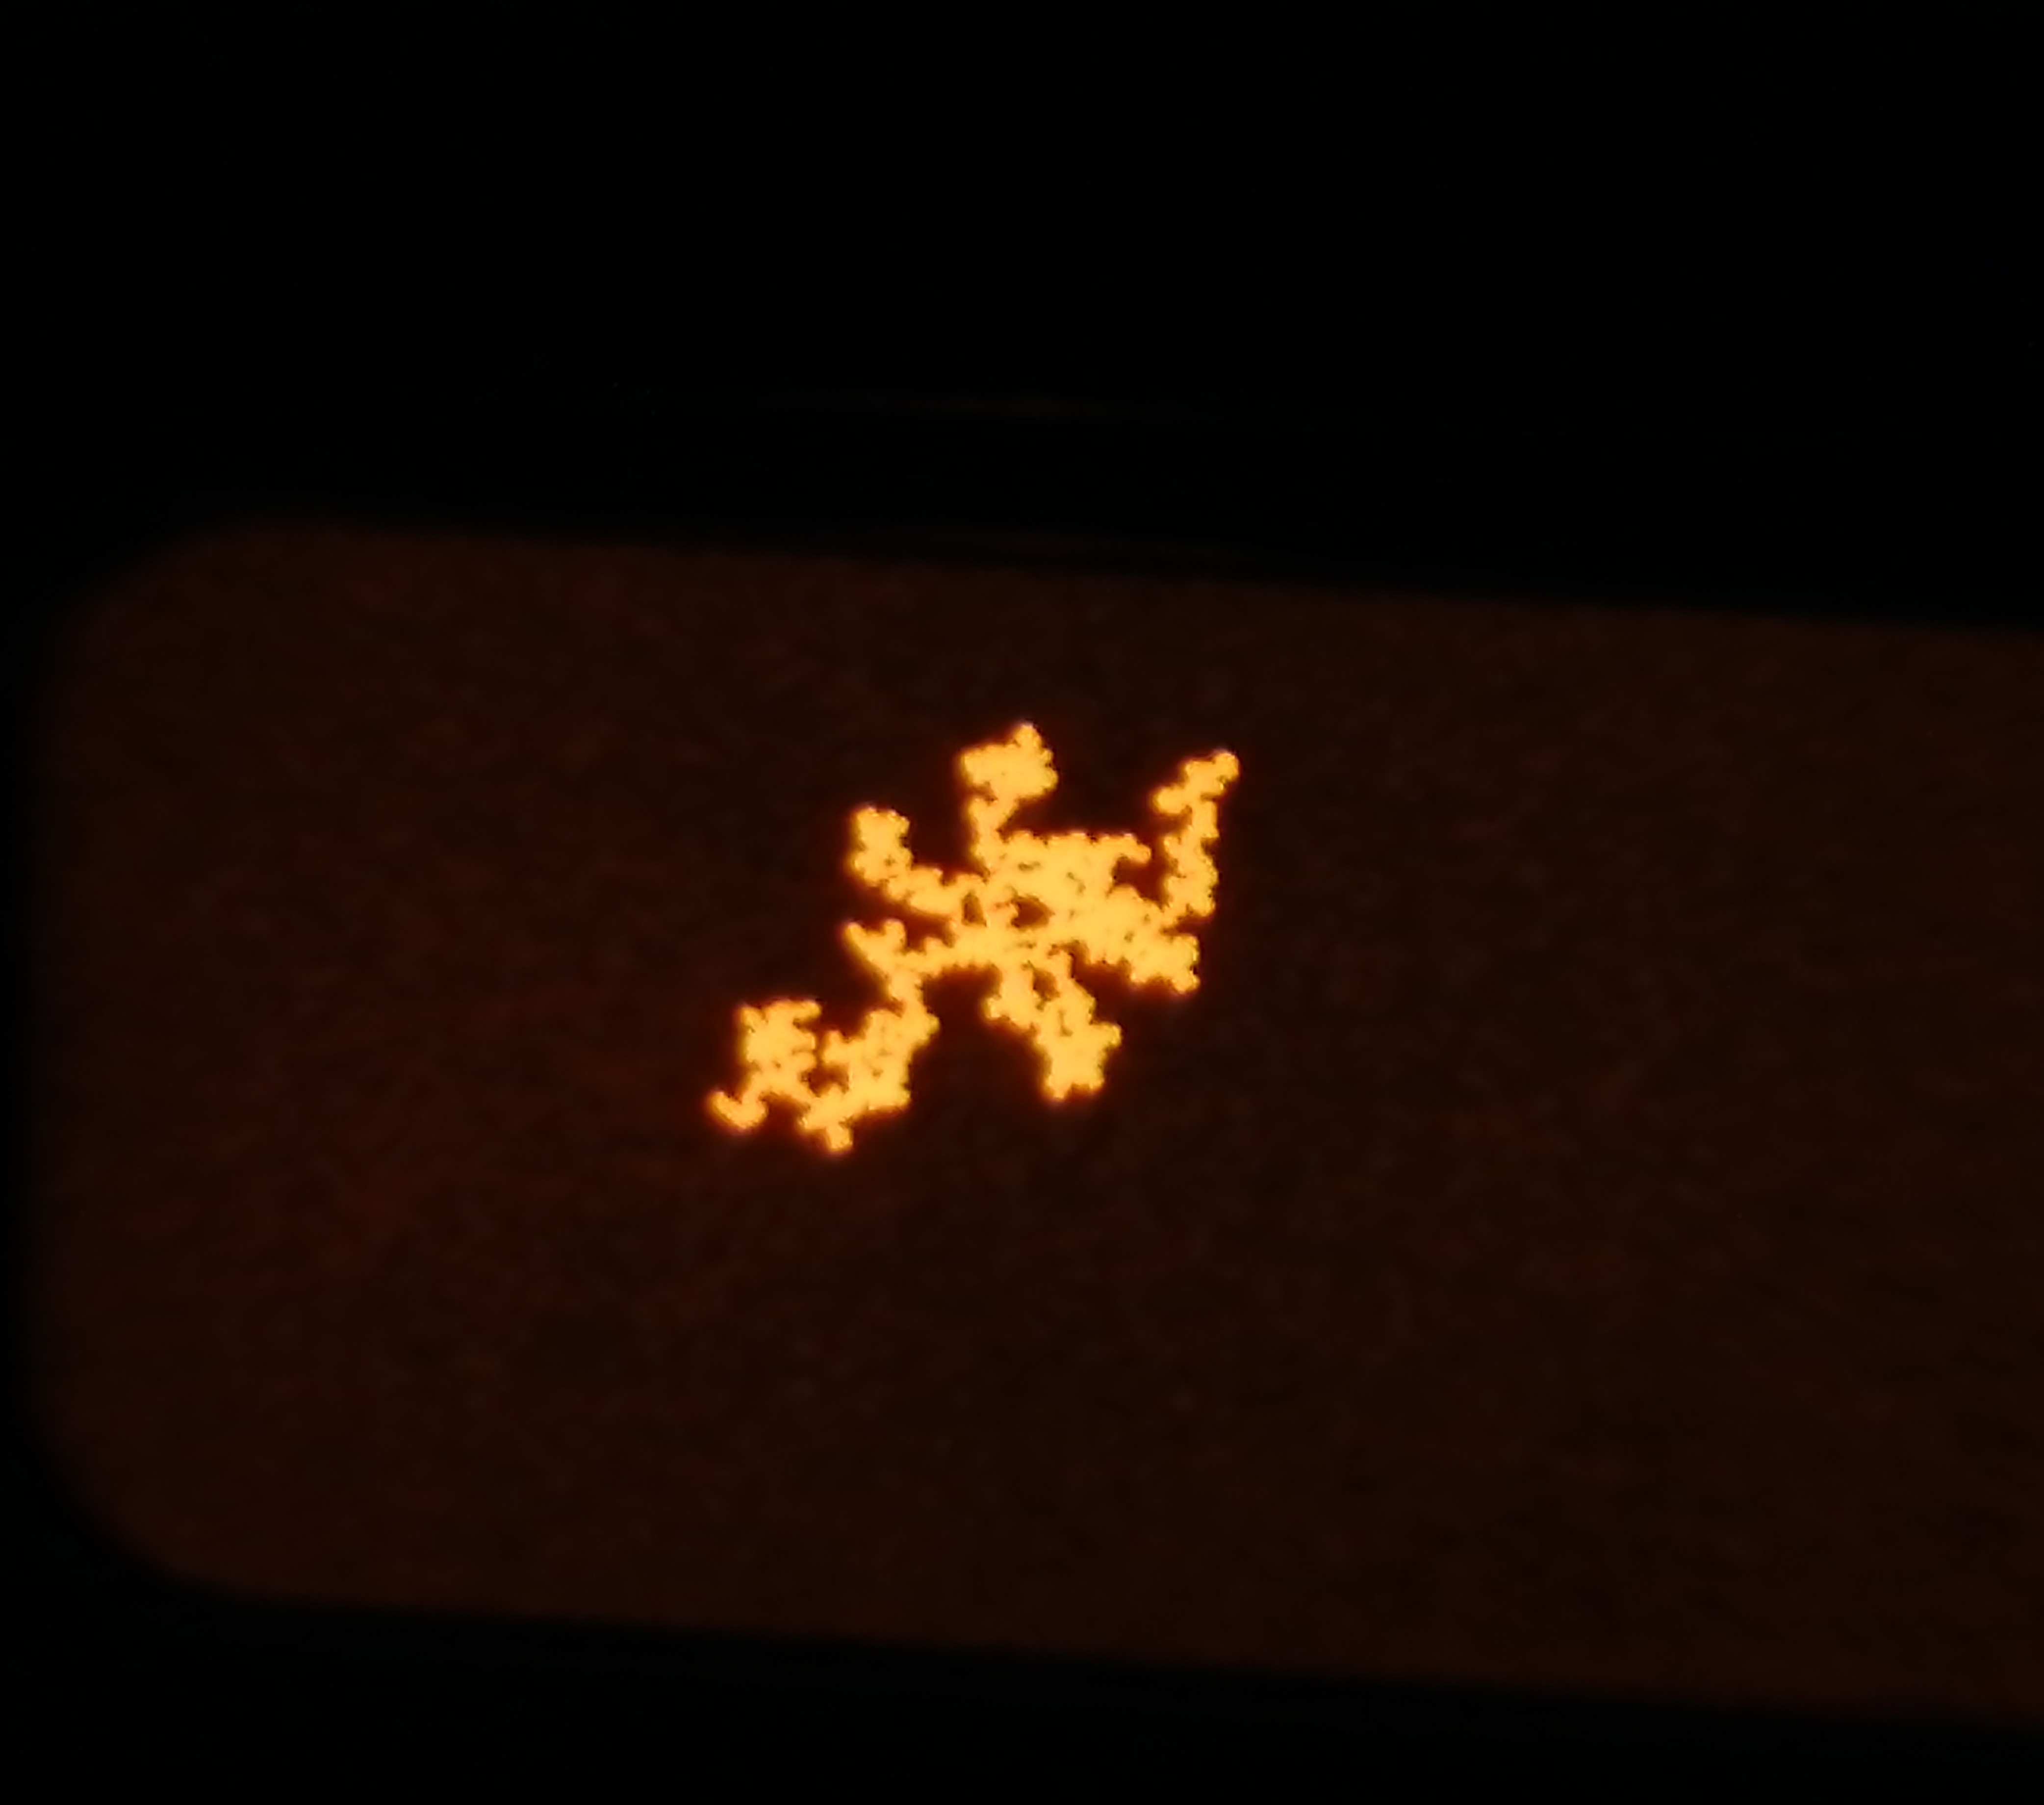
\includegraphics[width=.9\linewidth]{images/display.jpg} 
		\caption{light on} 
	\end{subfigure}
	\begin{subfigure}[b]{.45\textwidth}
		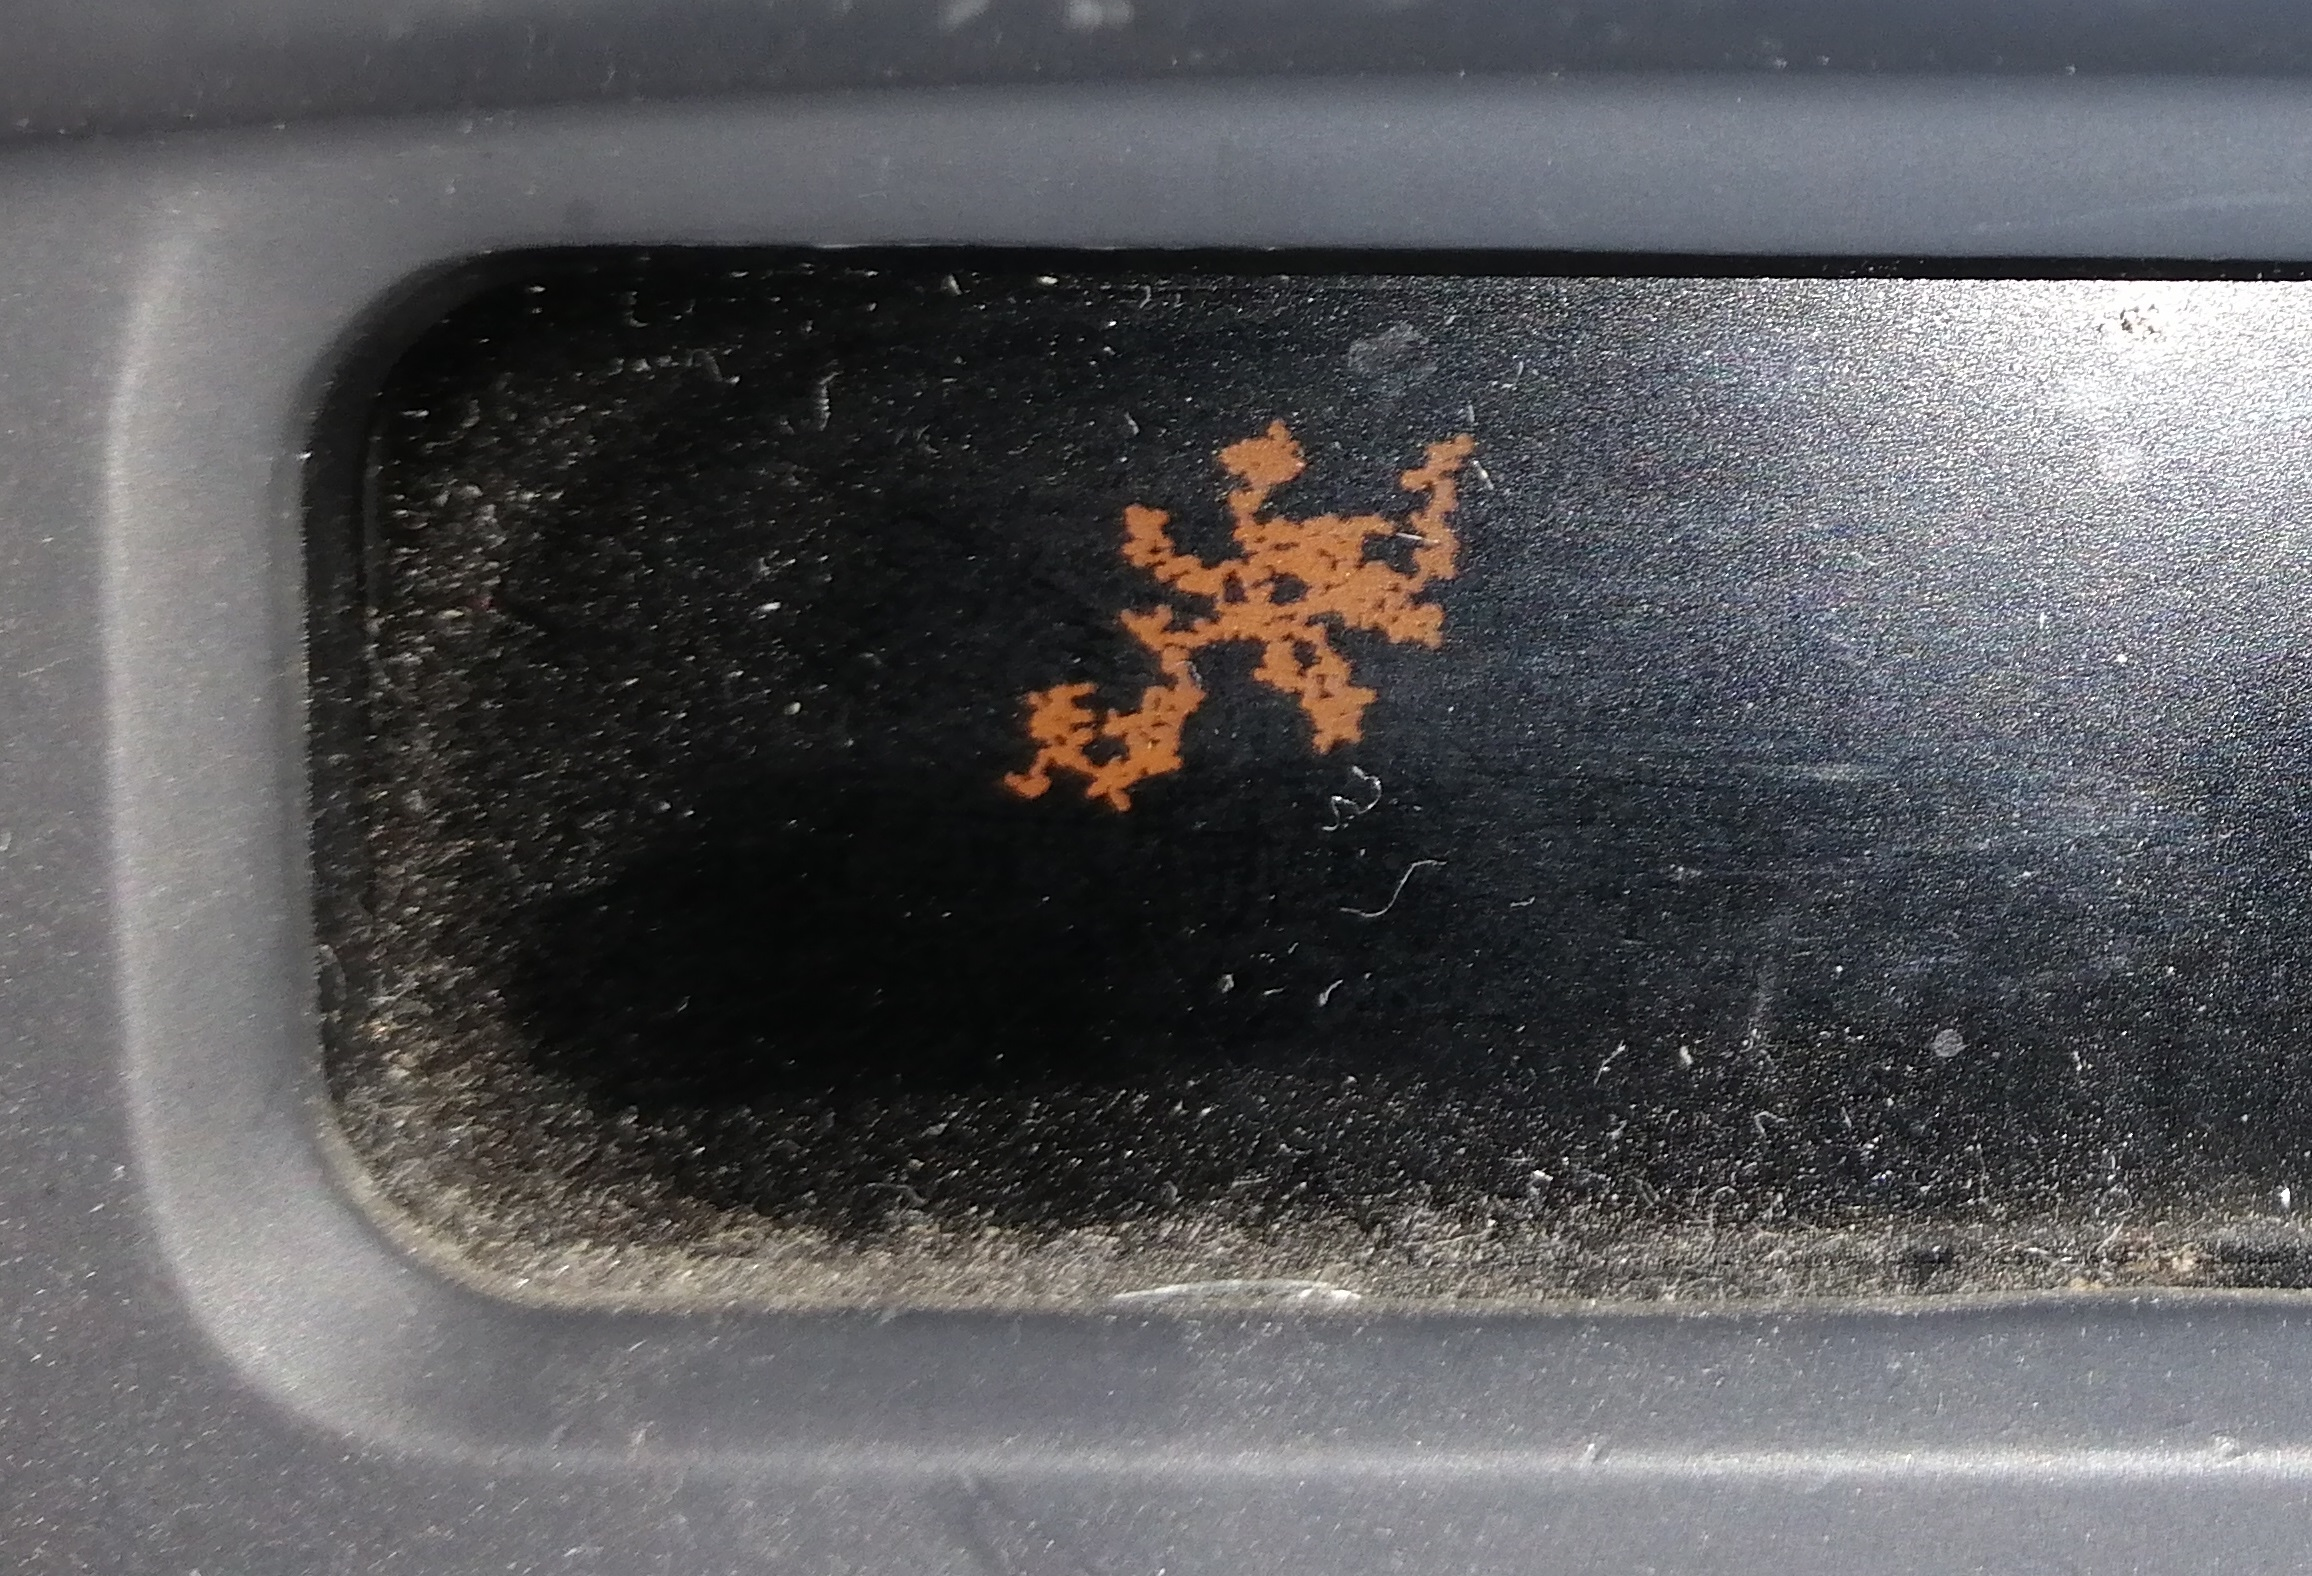
\includegraphics[width=.9\linewidth]{images/display2.jpg}
		\caption{light off} 
	\end{subfigure}
	\caption{Cluster appearance in the radio screen of a car}
	\label{radio}
\end{figure}

\begin{figure}
	\begin{subfigure}[b]{.45\textwidth}
		
\includegraphics[width=1\linewidth]{images/snowflake.jpg}
		\caption{Real snowflake crystal, see at \cite{snowflake}} 
	\end{subfigure}
	\begin{subfigure}[b]{.45\textwidth}
		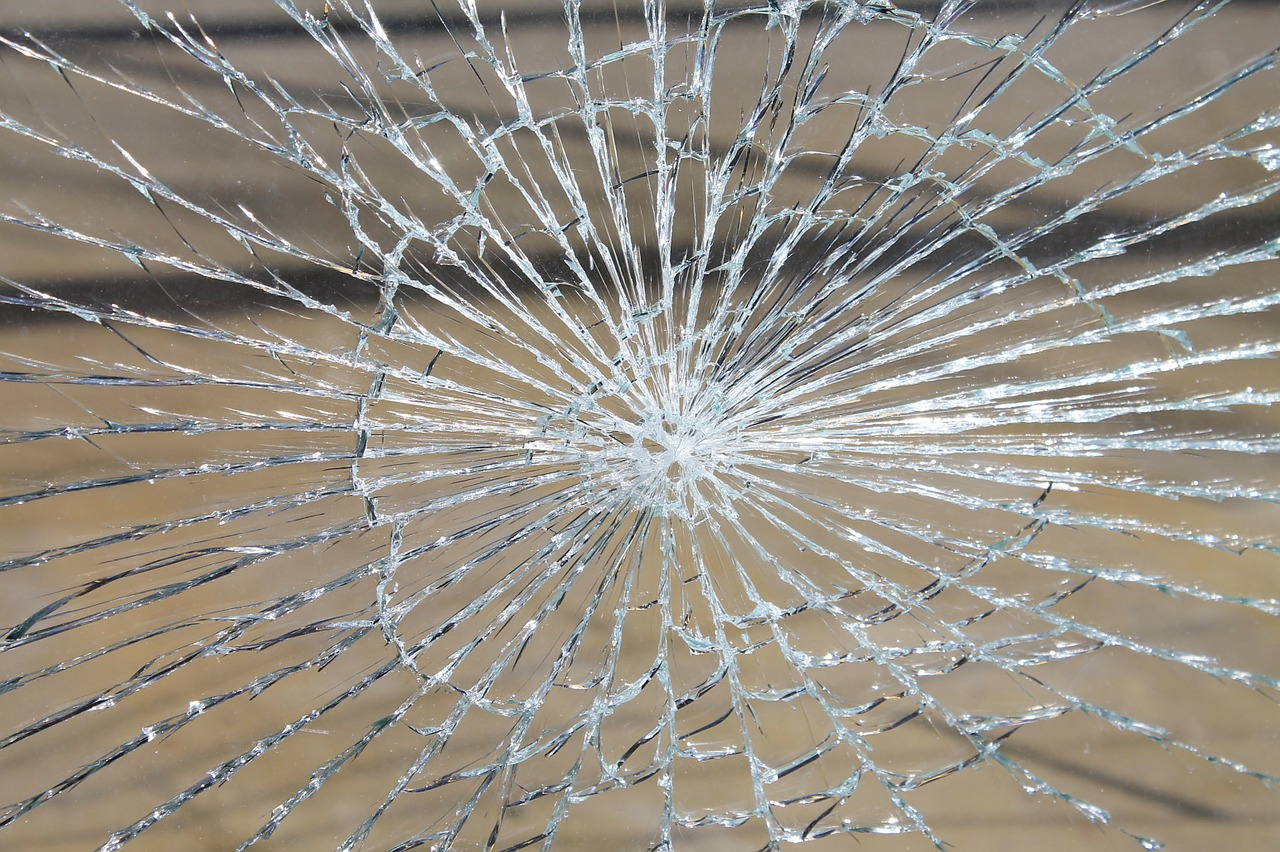
\includegraphics[width=.8\linewidth]{images/glass-break.jpg}
		\caption{Broken glass} 
	\end{subfigure}
	\caption{Other examples}
	\label{other}
\end{figure}




\newpage


\section{Preliminaries} \label{prelim}

\subsection{Symbols}
Let $d\in \N$ and $q\in \{0,\dots,d\}$. 
\begin{flalign*}
	&\N = \{1,2,3,\dots\},\quad \text{the set of natural numbers (without 0)}\\
	&\N_0 = \N\cup\{0\}\\
	&\N^\infty = \N \cup \{\infty\}\\
	&\mathcal{B}^d,\quad \text{$d$-dimensional Borel-$\sigma$-algebra of $\R^d$} \\
	&\K^d,\quad \text{the set of convex and compact sets in }\R^d\\
	&B_d(x,r) = \{y\in \R^d\ |\ |x-y| \leq r\},\quad  \text{the $d$-dimensional closed ball of radius $r$ around $x$}\\
	&B_r := B_2(r,0) \\
	&S_{d-1}(r,x) = \partial B_d(r,x),\quad  \text{the $(d-1)$-dimensional surface of the $d$-dimensional ball}\\
	&A(d,q),\quad \text{the set of q-dimensional affine subspaces of }\R^d \\
	&\mathcal{A}(d,q),\quad  \text{the $\sigma$-algebra of } A(d,q), \text{ as constructed later in the paper} \\
	&\G := A(2,1),\quad  \text{the set of lines in the real plane}\\
	&SO_d := \{\nu \in \R^{d\times d}\ |\ \nu \nu^\top = I_d \text{ and } \det \nu = 1\},\quad \text{identify }SO_2 = \{\nu_\beta := e^{i\beta} \in \C\ |\ \beta\in [0,2\pi)\} \\
	&G_d := \{\varphi: \R^d \to \R^d, x\mapsto \nu x+b\ |\ \nu \in SO_d,b\in \R^d\},\quad  \text{the set of euclidean motions} \\
	&\mP^d_f,\quad \text{the set of finite subsets of $\Z^d$} \\
	&\mP_f := \mP^2_f 
\end{flalign*}

\noindent Note that we will always identify $\R^2$ with $\C$ ($(a,b)\leftrightarrow a+bi$) for a more convenient notation. 

\subsection{Expressions}

Throughout the paper let  $(\Omega,\mathcal{F}, \mathbb{P})$ be a probability space. If for $A\in \mathcal{F}$ we have $\mathbb{P}(A)=1$ we will say that \glqq $A \text{ holds }\mathbb{P}\text{-a.s.}$\grqq, or short \glqq$ A\text{ holds } \text{a.s.}$\grqq ($A$ holds almost surely). Another short expression, if for a set of logical statements $(A_t)_{t\in I}$ with $I\in\{\N,\R\}$ we say \glqq $A_t$ holds for large $t$\grqq\ it shall mean that there exists a $T\in I$ such that $A_t$ holds for all $t>T$. Here we mean that a logical statement holds if and only if the statement is true. 


\subsection{Graphs} \label{zgraph}

Let $d\in \N$. We will be interested in the undirected graph $(\mathbb{Z}^d, E)$ with its canonical graph structure, which is two vertices (or points) $x=(x_1,\dots,x_d),y=(y_1,\dots,y_d)\in \mathbb{Z}^d$ form an edge (e.q. $\{x,y\}\in E$) if and only if there exists exactly one $i\in \{1,\dots, d\}$ such that $|x_i - y_i| = 1$ and $x_j = y_j$ for all $j\neq i$. For a point $x\in \mathbb{Z}^d$ its set of $\mathit{neighbours}$ is defined as 
\begin{align*}
	N(x) := \{y\in \mathbb{Z}^d\ |\ \{x,y\}\in E\}.
\end{align*}
For a set $A\subset \mathbb{Z}^d$ the $\mathit{outer\ boundary}\ \partial A$ of $A$ is defined as 
\begin{align*}
	\partial A := \{y\in \mathbb{Z}^d\setminus A\ |\ \exists x\in A:\ \{x,y\}	\in E\}
\end{align*}
and the closure $\bar A$ of $A$ as 
\begin{flalign*}
	\bar A := A\cup \partial A.
\end{flalign*}
Instead of $(\mathbb{Z}^d, E)$ we will write $\mathbb{Z}^d$ from now on. 

\subsection{Random Walks}

\begin{definition}
	 For our space of interest $\mathbb{Z}^d$ we will always use the discrete $\sigma$-algebra which is the power set of $\mathbb{Z}^d$. A family $(S_n)_{n\in \mathbb{N}_0}$ of measurable functions $S_n: \Omega \to \mathbb{Z}^d$ is called a $\mathit{random\ walk\ on}\ \mathbb{Z}^d$ $\mathit{(starting\ at}\ x\in \mathbb{Z}^d)$ if and only if $S_0=x$ a.s. and 
	
	\begin{align*}
		\mathbb{P}(S_n = y\ |\ S_{n-1} = z) = \frac{1}{|N(z)|} = \frac{1}{2d},\quad \text{ for all }  y\in N(z) \text{ and } z\in \Z^d.
	\end{align*}
	
	\noindent Note that $|N(z)| = 2d$ for all $z\in \mathbb{Z}^d$ since every point has two neighbours in the direction of every dimensional component. We can therefore conclude easily that $\mathbb{P}(S_n = y\ |\ S_{n-1} = z) = 0$ for all $y\notin N(z)$ and $z\in \Z^d$. For $x,y\in\Z^d$ we introduce the short notation
	\begin{flalign*}
		\PP_x(S_n=y) := \PP(S_n = y\ |\ S_0 = x). 
	\end{flalign*}
	
\end{definition}
So a random walk can be understood as a particle starting from some point $x$ and moving randomly on the grid choosing its next step uniformly from its neighbours. For the following let $(S_n)_{n\in \mathbb{N}}$ be a random walk on $\Z^d$ starting at $x\in \Z^d$. 

\begin{definition}
	Let $A\subset \Z^d$. We define the $hitting\ times$ of A by
	
	\begin{align*}
		T_A := \min \{n\geq 0\ |\ S_n\in A\}\text{ and } T^+_A := \min \{n\geq 1\ |\ S_n\in A\}, 
	\end{align*}
	
	\noindent and $T_y:= T_{\{y\}}$ and $T^+_y:= T^+_{\{y\}}$ for $y\in \Z^d$.
\end{definition}

\begin{definition}
	A random walk with origin in $x\in\Z^d$ is called  $\mathit{recurrent}$ if
	\begin{flalign*}
		\PP_x(T^+_x<\infty) = 1
	\end{flalign*}
	and $\mathit{transient}$ if
	\begin{flalign*}
		\PP_x(T^+_x<\infty) < 1.
	\end{flalign*}
\end{definition}

\begin{lemma} \label{recurr}
	A random walk on $\Z^d$ is recurrent if $d\leq 2$ and transient if $d\geq 3$. 
\end{lemma}
\begin{proof}
	Proofs of this result are presented in $\cite{henze}$ Satz $5.1$ or $\cite{markov}$ Korollar $2.6.6$. 
\end{proof}

\begin{lemma} \label{recurrA}
	The following two statements are equivalent:
	\begin{enumerate}
		\item $\PP_x(T_x^+<\infty) = 1 \text{ for all } x\in\Z^2$
		\item $\PP_x(T_A^+<\infty) = 1 \text{ for all } x\in\Z^2 \text{ and } A\subset\Z^2$
	\end{enumerate}
\end{lemma}

\begin{proof}
	The direction $(ii)$ to $(i)$ is clear. For the other direction choose $x\in\Z^2$ and $A\subset \Z^2$. We know that in general for any point $y\in\Z^2$ we have $\PP_x(T_y^+<\infty) > 0$ for a random walk in $\Z^d$ for any dimension $d\in\N$. By Lemma \ref{recurr} we know that a random walk on $\Z^2$ is recurrent. For that case it is proved  in \cite{markov} Satz $2.6.9$ that $\PP_x(T_y^+<\infty) = 1$ holds for even any $y\in\Z^2$. If we choose $y\in A$ we get
	\begin{flalign*}
		1 = \PP_x(T_y^+<\infty) \leq \PP_x(T_A^+<\infty),
	\end{flalign*}
	which completes the proof. 
\end{proof}

After having introduced some basics we will in the next chapter turn our focus to the main definition of stochastic processes we will discuss in this paper. 



\newpage
\section{Incremental Aggregation}

\subsection{Definition}

In this paper we will look at stochastic processes on the set of finite subsets of $\mathbb{Z}^2$, where we start with the one point set $\{0\}$ and incrementally add a point of the outer boundary of the current cluster according to some distribution. What we get is a randomly, point by point growing connected cluster which we will call $\mathit{incremental\ aggregation}$. Define 
\begin{flalign*}
	\mP_f := \{A\subset \mathbb{Z}^2\ |\ \text{A is finite}\}, 
\end{flalign*}
the set of finite subsets of $\mathbb{Z}^2$. Furthermore we will be interested in distributions on those sets, so for $A\in \mP_f$ we define 
\begin{flalign*}
	\mathcal{D}_A:= \{\mu: \mathbb{Z}^2\to [0,1]\ |\ \mu(y) = 0 \text{ for all } y\notin A\ \text{and}\ \sum_{y\in A} \mu(y) = 1 \}, 
\end{flalign*}
the set of distributions on $A$. Now we define incremental aggregation as follows.  

\begin{definition} \label{incrementalaggregation}
	Let $\mu=(\mu_A)_{A\in \mP_f}$ be a family of distributions with $\mu_A\in \mathcal{D}_A$ for all $A\in \mP_f$. An $\mathit{incremental\ aggregation\ (with\ distribution\ \mu)}$ is a stochastic process $(\mathcal{E}_n)_{n\in{\mathbb{N}}}$ which evolves as follows. The process starts with one point $\mathcal{E}_1 = \{0\}$ (define $y_1 :=0$) at the origin of $\mathbb{Z}^2$. Knowing the process $\mathcal{E}_n$ at time $n$, let $y_{n+1}$ be a random point in $\partial \mathcal{E}_n\in \mP_f$ with distribution
	\begin{align}
		\mathbb{P}(y_{n+1} = y\ |\ \mathcal{E}_n) := \mu_{\partial \mathcal{E}_n}(y),\quad y\in \mathbb{Z}^2.
	\end{align}
	We then define $\mathcal{E}_{n+1} := \mathcal{E}_n \cup \{y_{n+1}\}$ and the limit cluster as $\E_\infty := \bigcup_{n\in\N} \E_n$. This defines a Markov chain whose state space is the set of finite and connected subsets of $\Z^2$. 
\end{definition} 

\begin{remark} \label{orderindependence}
	It is worth to mention that the distribution of a new added point $y_{n+1}$ is not depending on the order of how previous points where added to the cluster since the functions $\mu_A$ only look at the boundary of the current cluster and therefore do not consider any information about orderings of cluster points. 
\end{remark}



\subsection{Notion of Fractal Dimension and Growth Rate} \label{notion}

\begin{figure}
	\centering
	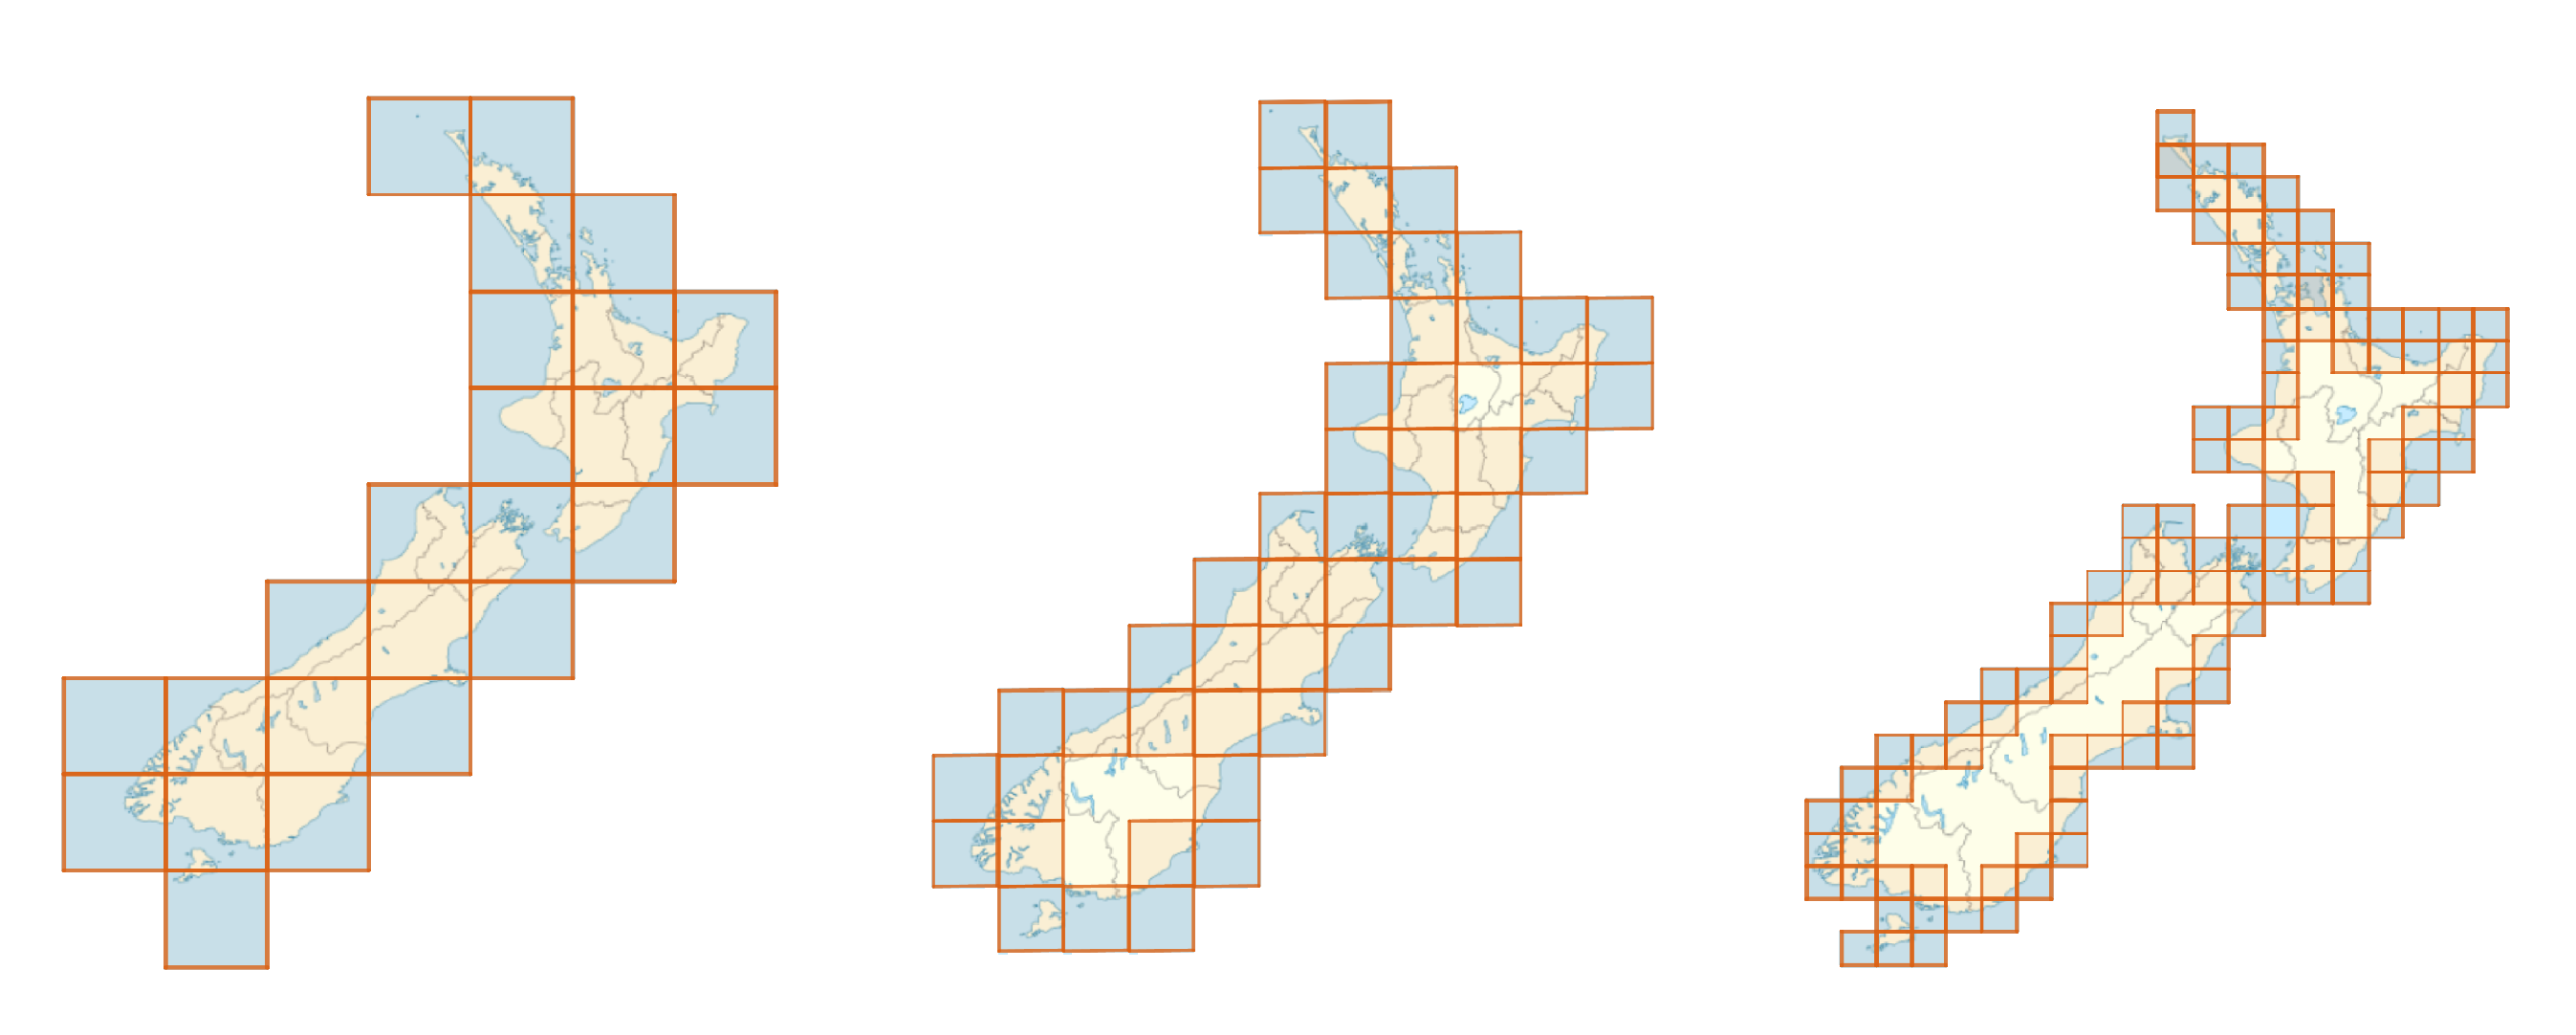
\includegraphics[height=6.5cm]{images/geogebra-images/neuseeland-squares.png}
	\caption{Box-covering of New Zealands outer cost with decreasing box sizes $\varepsilon$} \label{neuseeland}
\end{figure}

The notion of fractal dimension is usually used for sets with uncountable cardinality like continuous curves or surfaces. One way of defining a fractal dimension for curves like for example the cost line of New Zealand (see \autoref{neuseeland}) would be to look at the limit relation between the minimum number of boxes (squares) which we need to cover the cost line and the side length of these boxes. The following definition is motivated by \cite{hausdorff} page 160. If for $\varepsilon>0$ $N(\varepsilon)$ is the mininum number of boxes with side length $\varepsilon$ which we need to cover the cost line, then the so called $\mathit{box\text{-}dimension\ d_b}$ is a constant such that $N(\varepsilon)$ grows as fast as $\varepsilon^{-d_b}$ for letting $\varepsilon$ tend to zero, so 
\begin{flalign} \label{boxdimension}
	d_b := - \lim_{\varepsilon\to 0} \frac{\ln(N(\varepsilon))}{\ln(\varepsilon)}. 
\end{flalign} 

This definition makes sense in many contexts, for example is the box-dimension of straight line segments $1$ and of squares $2$ and so on, so in those cases equal to the topological dimension. As with incremental aggregations we are dealing with finite point sets, this approach of defining a fractal dimension for our clusters is not senseful. It is not difficult to show, that the box-dimension of any finite set is $0$. A helpful detail about the situation with finite sets as the ones we are looking at is that each point of the cluster can actually be interpreted and identified with a unique square since the cluster is living on the grid $\Z^2$. We will precise that in chapter \ref{lha}. So instead of decreasing the sizes of the boxes with which we cover our set of interest, we leave the size of the boxes constant and increase the size of our set by adding points and looking at the limit cluster $\E_\infty$. 
Defining the radius of a finite set $A\in \mP^d_f$ (with $|\cdot|$ the euclidean norm) as 
\begin{flalign} \label{radius}
	\rad(A) := \max_{x\in A} |x|,
\end{flalign}
we therefore can identify the relation between the geometrical sizes of the boxes and the cluster as follows. For $n\in\N$ define $\varepsilon_n:=\frac{1}{\EE[\rad(\E_n)]}$. Before $\varepsilon_n$ would have expressed the geometrical relation between one box and the whole cluster which we describe now by the fraction $\frac{1}{\EE[\rad(\E_n)]}$ since a box size is now constantly $1$ and the clusters geometrical size we can interpret by $\EE[\rad(\E_n)]$ up to a constant. That analogy makes even more sense if the cluster happens to be self-similar in some way looking at different sizes of it. The minimum number of boxes with size $1$ with which we need to cover $\E_n$ is always $n$, so $N(\varepsilon_n)=n$ for all $n\in\N$ and therefore we can rewrite the definition of the box-dimension (\ref{boxdimension}) by replacing $\varepsilon_n$ with $\frac{1}{\EE[\rad(\E_n)]}$ and define the $\mathit{(discrete)\ fractal\ dimension}$ of $\E_\infty$ as
\begin{flalign} \label{fractaldimension}
	d_f := \liminf_{n\to\infty} \frac{\ln(n)}{\ln(\EE[\rad(\E_n)])}
\end{flalign}
Another way of tackling the intuition for a fractal dimension of discrete sets is by considering subsets of the $d$-dimensional ball $B_d(0,m)$ of radius $m\geq 0$, which is motivated by $\cite{fractalwinter}$ Part II page 98 and $\cite{lawler}$ 2.6 page 82. If we take a finite subset $M$ of that ball, we could assign it the dimension $k$ if its cardinality is of order $m^k$. If we apply the same argument to the clusters $\E_n$ and balls with radius $\EE[\rad(\E_n)]$ for all $n\in\N$, we get that the dimension of $\E_\infty$ could be interpreted as a constant $k$ which fulfills that $n=|\E_n|$ grows as fast as $\EE[\rad(\E_n)]^k$ for letting tend $n$ to infinity. We therefore get the same definition as in (\ref{fractaldimension}). This way of defining a fractal dimension for incremental aggregations strongly correlates with the growth rate of the aggregation which shall indicate how the radius of the cluster evolves while increasing the particle number. We can define the growth rate by looking for the smallest exponent $\alpha$ such that there exists a constant $c>0$ with 
\begin{flalign*}
	\EE [\rad(\E_n)] \leq cn^\alpha
\end{flalign*}
for large $n$. Rewriting this we come to the equivalent inequality
\begin{flalign*}
	\frac{\ln(\EE [\rad(\E_n)])}{\ln(n)} - \frac{\ln(c)}{\ln(n)} \leq \alpha
\end{flalign*}
for large $n$ and we could finally define the growth rate $\alpha_f$ of an incremental aggregation as the smallest value satisfying this inequality, so
\begin{flalign} \label{growthrate}
	\alpha_f := \limsup_{n\to\infty} \frac{\ln(\EE [\rad(\E_n)])}{ln(n)}.
\end{flalign}
We therefore simply get that 
\begin{flalign} \label{fractaldim}
	d_f = \frac{1}{\alpha_f},
\end{flalign}
which includes the cases $d_f=\infty$ or $\alpha_f=\infty$ ($\frac{1}{0}:= \infty)$, which in total motivates choosing the limes inferior in the definition (\ref{fractaldimension}). Since $\rad(\E_n) \leq n$ for all $n\in\N$ a.s., we get 
\begin{flalign*}
	\alpha_f \leq 1. 
\end{flalign*}
and therefore 
\begin{flalign*}
	d_f \geq 1.
\end{flalign*}
In $\Z^d$ for some $d\in\N$ we can fill the cube with center $0$ and side length $n$ with an order of $n^{\frac{1}{d}}$ points. Therefore we can fill the ball of radius $n$ with an order of $n^{\frac{1}{d}}$ points as well, so there is a constant $c>0$ such that $cn^{\frac{1}{d}} \leq \rad(\E_n)$ for all $n\in\N$ a.s.. Hence
\begin{flalign*}
	d_f \leq \liminf_{n\to\infty} \frac{\ln(n)}{\ln(cn^{\frac{1}{d}})} = d.
\end{flalign*}
So in total we get the trivial boundaries
\begin{flalign}\label{trivialboundary}
	1\leq d_f \leq d 
\end{flalign}
and
\begin{flalign*}
	\frac{1}{d}\leq \alpha_f \leq 1
\end{flalign*}
for any incremental aggregation in $\Z^d$. \\

\begin{remark}
	If we define the fractal dimension as in \ref{fractaldimension} we encounter the problem that when the cluster reaches some radius the first time in many instances there will still particles be added to the cluster without increasing its radius, so to say \glqq $\text{filling}$\grqq\ the cluster up to that radius. If the fractal dimension shall indicate a limit relation between how many particles of the final cluster $\E_\infty$ lie in a ball of a radius letting the radius tend to infinity, our definition in \ref{fractaldimension} does not reflect that directly. Nevertheless it seems to make sense that these two situations are equivalent which we state more clearly in the following conjecture. 
\end{remark}

\begin{conjecture}
	Let $B_n$ be a ball of radius $n\in\N$ with center $0$ and with $\E_\infty \cap B_n$ denote the set of particles in $\E_\infty$ that lie in $B_n$. Note that $n-2 \leq \rad(\E_\infty \cap B_n)\leq n$. Then we have
	\begin{flalign*}
		d_f = \limsup_{n\to\infty} \frac{\ln(\EE |\E_\infty \cap B_n|)}{\ln(n)}
	\end{flalign*}
\end{conjecture}

BILD

\newpage
\section{External Diffusion Limited Aggregation}

\subsection{Definition}

External DLA is a model of an incremental aggregation as defined above using a very natural family of distributions, called the $\mathit{harmonic\ measures}$. 

\begin{definition} \label{harmonicmeasure}
	$\mathit{(harmonic\ measure)}$ Let $A\subset\Z^d$. The hitting probability of $A$ is the function 
	\begin{flalign*}
		H_A: \Z^d \times A \to [0,1],\quad (x,y) \mapsto H_A(x,y):=\PP_x(S_{T_A^+} = y).
	\end{flalign*}
	In literature you can find the same definition where $T_A$ is used instead of $T_A^+$. Since in the following for finite sets $A\in\mP^d_f$ the limit $|x| \to \infty$ of $H_A(x,y)$ is of interest, $T_A^+$ is chosen for convenience. In fact, for a fixed element $x\in\Z^d$ the function $H_A(x,\cdot)$ defines a measure on $A$ with total mass $\PP_x(T_A^+<\infty)$ and it can be adapted to a probability measure by conditioning the random walk to hit $A$ in finite time. Define
	\begin{flalign*}
		\bar H_A: \Z^d \times A \to [0,1],\quad (x,y) \mapsto \bar H_A(x,y):=\PP_x(S_{T_A^+} = y\ |\ T_A^+<\infty), 
	\end{flalign*} 
	so for fixed $x\in\Z^d$ the function $\bar H_A(x,\cdot)$ defines a probability measure on $A$. Indeed this definition is motivated by $\cite{lawler}$ (Chapter $2$, Definition $2.1$) and in the same chapter it is proved, that for finite sets $A\in\mP^d_f$ the limit
	\begin{flalign*}
		\lim_{|x|\to\infty} \bar H_A(x,y) =: h_A(y) 
	\end{flalign*}
	exists for each $y\in A$. The function $h_A: A\to [0,1]$ is called the $\mathit{harmonic\ measure\ of\ A}$. For an element $y\in A$, $h_A$ can be interpreted as the probability that a random walk starting at \glqq $\text{infinity}$\grqq hits $A$ the first time at $y$.
\end{definition}

\begin{definition} $\mathit{(external\ diffusion\ limited\ aggregation)}$ $\mathit{External\ diffusion\ limited}$ $\mathit{aggregation}$ (on $\Z^d$), short $\mathit{external\ DLA}$ or just $\mathit{DLA}$, is an incremental aggregation with the family of harmonic measures $(h_A)_{A\in\mP^d_f}$ as distribution. 
\end{definition}

\begin{remark} \label{harmonicmeasure2}
	If we look at the $2$-dimensional case, by Lemma $\autoref{recurrA}$, we have that $\PP_x(T_A^+<\infty) = 1$ for any $x\in\Z^2$, and therefore get $\bar H_A = H_A$. So in two dimensions the harmonic measure of $A\subset \Z^2$ can be written as 
	\begin{flalign*}
		h_A(y) = \lim_{|x|\to\infty} \PP_x(S_{T_A^+} = y), \quad y\in A. 
	\end{flalign*}
\end{remark}


\subsection{Fractal Dimension and Growth Rate of External DLA in $\Z^2$}

There is not yet a rigorous proof on the exact fractal dimension of external DLA. There are rather few rigorously proved results and it seems that it is very hard to prove such results on DLA. Looking at computer simulations of DLA in $\Z^2$ it seems that the clusters are relatively sparse and they appear to have a noninteger fractal dimension. In $\cite{magnetic}$ DLA is observed in a magnetic aggregation context, and empirically they find a fractal dimension of around $1.8$. Other simulations seem to suggest a value a little less than 1.7 for $d_f$ in two dimensions ($\cite{lawler}$ page 83). There is also a theory that predicts 
\begin{flalign*}
	d_f = \frac{d^2 + 1}{d+1}
\end{flalign*}
in $\Z^d$ which seems to agree fairly well with simulations ($\cite{lawler}$ page 83). There are only few rigorously proved results and we will see one of them in the following. First we will proof some lemmas. For that define two random functions
	\begin{flalign*}
		r: \N \to [0,\infty),\quad n\mapsto \rad(\E_n)
	\end{flalign*}
	and
	\begin{flalign*}
		T: [0,\infty) \to \N,\quad s\mapsto \min\{j\in\N\ |\ r(j)\geq s\}.
	\end{flalign*}
	Remind that $\rad(\E_n)$ is the radius of the cluster at time $n$ as defined in \ref{notion} (\ref{radius}). 
\begin{remark}\label{props}
	It is easy to show that, for all $\omega\in\Omega$, $r(\omega)$ and $T(\omega)$ grow monotonously in $n\in\N$ resp. $s\in [0,\infty)$ and that for all $n\in\N$ and $s\in [0,\infty)$ we have $T(\omega)(r(\omega)(n)) \leq n$ and  $r(\omega)(T(\omega)(s)) \geq s$.
\end{remark}

\begin{lemma} \label{rtinfty}
	For both random functions $r$ and $T$ we have that
	\begin{flalign*}
		r(\omega)(n) \to\infty \text{ for } n\to\infty
	\end{flalign*}
	and
	\begin{flalign*}
		T(\omega)(s) \to\infty \text{ for } s\to\infty
	\end{flalign*}
	for all $\omega\in\Omega$.
\end{lemma}
\begin{proof}
	Since we are moving on the grid $\Z^d$ we have that for a ball $B_d(0,n)$ with radius $n\geq0$ the number $N:=|B_d(0,n)\cap \Z^d|$ is finite and for any $\omega\in\Omega$ we get 
	\begin{flalign*}
		r(\omega)(2N)\geq n. 
	\end{flalign*}
	Therefore for all $\omega\in\Omega$ and any $n\in\N$ we can find a $M\in\N$ such that $r(\omega)(M)\geq n$, and since $r(\omega)$ grows monotonously we get $r(\omega)(n) \to\infty \text{ for } n\to\infty$ for all $\omega\in\Omega$. Very similarly we can argue for $T$. 
\end{proof}

\begin{lemma} \label{randt}
	Let $a>0$ and $h:[0,\infty) \to [0,\infty)$ be a bijective, multiplicative and increasing function. For $c>0$ define
	\begin{flalign*}
		A_c:=\{\omega \in\Omega\ |\ \exists N=N(\omega)\in\N: r(\omega)(n) \leq ch(n) \text{ for all } n>N\}
	\end{flalign*}
	and
	\begin{flalign*}
		D_c := \{\omega \in\Omega\ |\ \exists N=N(\omega)\in\N: T(\omega)(as)\geq ch^{-1}(s) \text{ for all } s>N\}.
	\end{flalign*}
	 Then the following are equivalent:
	\begin{enumerate}
		\item $\exists c>0: \PP(A_c) = 1$ 
		\item $\exists c>0: \PP(D_c)=1$
	\end{enumerate}
\end{lemma}

\begin{proof} 
	$\Rightarrow$: 
	
	Choose $c>0$ such that $\PP(A_c)=1$. Take $\omega\in A_c$ and choose $N\in\N$ such that $r(\omega)(n)\leq ch(n)$ for all $n>N$. Hence there exists $\tilde c>0$ such that $\tilde ch^{-1}(r(\omega)(n))\leq n$ for all $n>N$. By Lemma \ref{rtinfty} we can choose $M\in\N$ big enough such that $T(\omega)(aM) > N$, hence $T(\omega)(as)\geq T(\omega)(aM) > N$ for all $s>M$ since $T(\omega)$ grows monotonously. Hence we can write $\tilde c h^{-1}(r(\omega)(T(\omega)(as))) \leq T(\omega)(as)$ for all $s>M$ and since $r(T(\omega)(as))\leq as$ we finally get $\tilde c h^{-1}(a)h^{-1}(s)=\tilde ch^{-1}(as) \leq T(\omega)(as)$ for all $s>M$, hence $\omega \in D_{\tilde c h^{-1}(a)}$, where we used the multiplicativity of $h$ and that $h^{-1}$ decreases monotonously. We therefore get $A_c\subset D_{\tilde c h^{-1}(a)}$, hence $\PP(D_{\tilde c h^{-1}(a)}) = 1$.\\
	$\Leftarrow$: 
	The proof for this direction works analogously and needs Lemma \ref{rtinfty} as well.
\end{proof}

\begin{lemma} \label{geometric}
	Let $n\in\N$, $n\geq 2$ and $T_1,\dots,T_n$ be independent geometrically distributed random variables with parameter $0<p<\frac{1}{2}$. Let $Y:=T_1 + \dots  + T_{n-1}$, then for every $a \in [2p,1)$ we have
	\begin{flalign*}
		\PP(Y\leq\frac{an}{p}) \leq \frac{1}{a} (ae^2)^n. 
	\end{flalign*}
\end{lemma}

\begin{proof}
	The moment generating function of $Y$ is
	\begin{flalign*}
		\EE[e^{tY}] = (pe^t)^{n-1}(1-e^t(1-p))^{-(n-1)} = p^{n-1}(e^{-t} - (1-p))^{-(n-1)}.
	\end{flalign*}
	By Chebyshev for any random variable $X$ we know the inequality
	\begin{flalign*}
		\PP(X\geq x) \leq \inf_{t>0} \frac{\EE[e^{tX}]}{e^{tx}}
	\end{flalign*}
	and can therefore follow that for any $t>0$ 
	\begin{flalign*}
		\PP(Y\leq \frac{an}{p}) = \PP(-Y\geq -\frac{an}{p}) \leq \exp(\frac{ant}{p})\EE[e^{-tY}] = \exp(\frac{ant}{p})p^{n-1}(e^t- (1-p))^{-(n-1)}. 
	\end{flalign*} 
	Choose $t=\ln(\frac{a(1-p)}{a-p})$ (note that $t>0$), then
	\begin{flalign*}
		\PP(Y\leq \frac{an}{p}) &\leq (\frac{a(1-p)}{a-p})^{\frac{an}{p}}   p^{n-1}   (1-p)^{-(n-1)}   (\frac{p}{a-p})^{-(n-1)} \\
		&= (\frac{a(1-p)}{a-p})^{\frac{an}{p}}  (1-p)^{-(n-1)}  (a-p)^{n-1} \\ 
		&= (\frac{a}{a-p})^{\frac{an}{p}} (1-p)^{\frac{an}{p}}  (1-p)^{-(n-1)}  (a-p)^{n-1} \\
		&\leq (\frac{a}{a-p})^{\frac{an}{p}}  (1-p)^{n-1}(1-p)^{-(n-1)}  (a-p)^{n-1} \\
		&\leq (1 + \frac{p}{a-p})^{\frac{2(a-p)n}{p}}a^{n-1} \\
		&\leq \frac{1}{a} (ae^2)^n.
	\end{flalign*}
\end{proof}

The following lemma gives a tool to handle conditioned probabilites and will be helpful later for developing splittings of probabilities similar to the law of total probability. 
\begin{lemma} \label{totalprob}
	Let $A,B\in\mathcal{F}$ with $\PP(B)>0$. Further let $c>0$ and $(C_i)_{i\in\N}\subset \mathcal{F}$ be a sequence of pairwise disjoint sets with $\PP(B\cap C_i)>0$, $\PP(A\ |\ B\cap C_i)\geq c$ for all $i\in\N$ and $B\subset \bigcup_{i\in\N} C_i$. Then
	\begin{flalign*}
		\PP(A\ |\ B) \geq c.
	\end{flalign*}
\end{lemma}

\begin{proof}
	We have
	\begin{flalign*}
		\PP(A\ |\ B) &= \frac{\PP(A\cap B)}{\PP(B)} = \frac{\PP(A\cap B\cap \bigcup_{i\in\N} C_i)}{\PP(B)} \\
		&= \sum_{i\in\N} \frac{\PP(A\cap B\cap C_i)}{\PP(B)} = \sum_{i\in\N} \frac{\PP(B\cap C_i)}{\PP(B)} \frac{\PP(A\cap B\cap C_i)}{\PP(B\cap C_i)} \\
		&= \sum_{i\in\N} \PP(C_i\ |\ B) \PP(A\ |\ B\cap C_i) \geq c \sum_{i\in\N} \PP(C_i\ |\ B) \\
		&= c.
	\end{flalign*}
\end{proof}

\begin{definition}
	For $x\in\Z^2$ and $r\in [1,\infty)$ define 
	\begin{flalign*}
		{\mP}^x_r := \{ A\in{\mP}_f\ |\ x\in A, r=\max_{y\in A} |x-y| \text{ and } A \text{ is connected}\}.
	\end{flalign*}
\end{definition}

The following theorem gives a bound on the harmonic measure which will be used in the proof we present here for the growth rate of DLA. The theorem is proved in $\cite{lawler}$ in Theorem $2.5.2$ and we state it slightly differently here to generalize it easier afterwards. 

\begin{theorem} \label{keytheorem}
	There exists a constant $c>0$ such that for all $r\in [1,\infty)$
	\begin{flalign*}
		h_A(0) \leq cr^{-\frac{1}{2}} \quad \text{ for all } A\in\mP^0_r.
	\end{flalign*}
\end{theorem}
\begin{proof}
	If $A\in\mP^0_r$ then $0\in A$ and $r=\rad(A)$ and for that case the proof is presented for all dimensions $d\in \N$ in $\cite{lawler}$ Theorem $2.5.2$. The proof is very technical and requires various results of other theorems and lemmas which are also to find in $\cite{lawler}$. 
\end{proof}

\noindent Theorem \ref{keytheorem} can be generalized as follows. 
\begin{proposition} \label{general}
	There exists a constant $c>0$ such that for all $y\in\Z^2$ and $s,r\in[1,\infty)$ with $s\geq r$ we have 
	\begin{flalign*}
		h_A(y) \leq cr^{-\frac{1}{2}} \quad \text{ for all } A\in\mP^y_s.
	\end{flalign*}
\end{proposition}

\begin{proof}
	For $y\in\Z^2$ define the translation function 
	\begin{flalign*}
		\Phi_y: \Z^2 \to \Z^2, x\mapsto x+y. 
	\end{flalign*}	
	Recall that in $\Z^2$ the harmonic measure of $A\subset\Z^2$ can be written as 
	\begin{flalign*}
		h_A(z) = \lim_{|x|\to \infty} \PP_x(S_{T_A^+} = z), \quad z\in A, 
	\end{flalign*}
	(see Remark \ref{harmonicmeasure2}). Since the distribution of random walks in $\Z^2$ is invariant under translation we can conlude that
	\begin{flalign*}
		h_A(z) &= \lim_{|x|\to \infty} \PP_x(S_{T_A^+} = z) \\
		&= \lim_{|x|\to \infty} \PP_{\Phi_y(x)}(S_{T_{\Phi_y(A)}^+} = \Phi_y(z)) \\
		&= h_{\Phi_y(A)}(\Phi_y(z)) 
	\end{flalign*}
	for all $z\in A$. By Theorem \ref{keytheorem} we know that there exists a constant $c>0$ such that for all $s\in[1,\infty)$ 
	\begin{flalign*}
		h_A(0) \leq cs^{-\frac{1}{2}} \quad \text{ for all } A\in\mP^0_s.
	\end{flalign*}
	Therefore for $s,r\in\R$ with $s\geq r$ we get 
	\begin{flalign*}
		h_A(0) = h_{\Phi_y(A)}(\Phi_y(0)) = h_{\Phi_y(A)}(y) \leq cs^{-\frac{1}{2}} \leq cr^{-\frac{1}{2}} \quad \text{ for all } A\in\mP^0_s, 
	\end{flalign*}
	and since $A\in\mP^0_s\ \Leftrightarrow\ \Phi_y(A) \in \mP^{\Phi_y(0)}_s$ we get
	\begin{flalign*}
		h_A(y) \leq cr^{-\frac{1}{2}} \quad \text{ for all } A\in\mP^y_s.
	\end{flalign*}
	Since $c$ was chosen independently of $y$, $s$ and $r$, this completes the proof. 
\end{proof}



\begin{theorem} \label{dlatheorem}
	For the fractal dimension of external DLA in $\Z^2$ as defined in section $\ref{notion}$ equation $(\ref{fractaldimension})$ we have
	\begin{flalign}
		d_f \geq \frac{3}{2}. 
	\end{flalign}	
\end{theorem}
\begin{proof}
	By section \ref{notion} equation (\ref{fractaldim}) we have
	\begin{flalign*}
		d_f = \frac{1}{\alpha_f},
	\end{flalign*}
	where $\alpha_f$ is the growth rate as defined in section $\ref{notion}$ equation $(\ref{growthrate})$, and we will therefore show that
	\begin{flalign*}
		\alpha_f \leq \frac{2}{3}.
	\end{flalign*}
	For $c>0$ define 
	\begin{flalign*}
		A_c := \{\omega\in\Omega\ |\ \rad(\E_n(\omega)) \leq cn^{\frac{2}{3}} \text{ for large }n\}
	\end{flalign*}
	and
	\begin{flalign*}
		D_c := \{\omega\in\Omega\ |\ T(\omega)(2n) \geq c n^{\frac{3}{2}} \text{ for large }n \}.
	\end{flalign*}
	If there is a constant $c>0$ such that
	\begin{flalign} \label{Ac}
		\PP(A_c) = 1, 
	\end{flalign}
	then we have
	\begin{flalign*}
		\alpha_f &= \limsup_{n\to\infty} \frac{\ln(\EE[\rad(\E_n)])}{\ln(n)}\\ &= \limsup_{n\to\infty} \frac{\ln(\int_\Omega \rad(\E_n) d\PP)}{\ln(n)} \\
		&= \limsup_{n\to\infty} \frac{\ln(\int_{A_c} \rad(\E_n) d\PP)}{\ln(n)} \\
		&\overset{(+)}{\leq} \limsup_{n\to\infty} \frac{\ln(\int_{A_c} cn^{\frac{2}{3}} d\PP)}{\ln(n)} \\ 
		&= \limsup_{n\to\infty} \frac{\ln(cn^{\frac{2}{3}})}{\ln(n)} \\
		&= \frac{2}{3} \limsup_{n\to\infty} \frac{\ln(c^{\frac{3}{2}}) + \ln(n)}{\ln(n)} = \frac{2}{3} \cdot 1 = \frac{2}{3}
	\end{flalign*}
	If we choose
	\begin{flalign*}
		h: [0,\infty) \to [0,\infty), x\mapsto x^{\frac{2}{3}},  
	\end{flalign*}
	and $a=2$, then by Lemma \ref{randt} we can show (\ref{Ac}) if we find a constant $c>0$ such that 
	\begin{flalign} \label{lambda}
		\PP(D_c) = 1. 
	\end{flalign}
	Note that $h$ is bijective, multiplicative and increasing. Lets first argue why the inequality at $(+)$ indeed holds. We define CONTINUE
	
	
	So now we will try to prove (\ref{lambda}). For $n\in\N$ write $\E_n = \{y_1,\dots,y_n\}$ according to Definition $\ref{incrementalaggregation}$, where $y_j$ is the $j$-th point added to the cluster. Let $\beta > 0$ which will be determined later on. For $n\in\N$ let $\tilde m_n := \beta n^{\frac{3}{2}}$ and define 
	\begin{flalign*}
		V_n := \{\omega\in\Omega\ |\ T(\omega)(2n) < \tilde m_n\}. 
	\end{flalign*}
	Further define the set of realised random walk paths of length $n$ with starting point in $\tilde B_n := \{x\in\Z^2\ |\ n \leq |x| < n+1\}$
	\begin{flalign*}
	Z_n := \{[z] := (z_1, \dots, z_n)\in (\Z^2)^n \ |\ z_1\in \tilde B_n, z_i\in N(z_{i-1}) \text{ for } i\in\{2,\dots,n\}\}, 
	\end{flalign*}
	for $[z]\in Z_n$ define events 
	\begin{flalign*}
		W_n([z]) := \{\omega\in\Omega\ |\ \exists j_1< \dots < j_n \leq \tilde m_n \ \text{ such that } y_{j_i}(\omega)  = z_i \text{ for all } i\in\{1,\dots,n\} \}
	\end{flalign*}
	and the union of these events 
	\begin{flalign*}
		W_n := \bigcup_{[z] \in Z_n} W_n([z]). 
	\end{flalign*}
	With $\tilde B_n$ we mean that the paths in $Z_n$ start \glqq on the boundary \grqq of $B_n$, the ball with radius $n$. We will quickly prove that 
	\begin{flalign*}
		V_n \subset W_n \text{ for all } n\in\N.
	\end{flalign*}
	Let $n\in\N$ and $\omega \in V_n$, then $T(\omega)(2n) < \tilde m_n$. For $m_n:=\max\{j\in\N\ |\ j\leq \tilde m_n\}$ we therefore have $T(\omega)(2n)\leq m_n$, hence $\rad(\E_{m_n}(\omega)) \geq 2n$. Therefore, since $\E_{m_n}(\omega)$ is connected, there must exist indices $j_1 <\dots < j_n$ such that $[z_0] := (y_{j_1}(\omega),\dots, y_{j_n}(\omega))\in Z_n$ and $[z_0]\subset \E_{m_n}(\omega)$, since $\max_{x\in [z_0]} |x| \leq 2n$. Therefore $j_n \leq m_n\leq\tilde m_n$ and therefore $\omega \in W_n([z_0]) \subset W_n$ which proofs the inclusion.\\ 
	\\ For a sequence of events $(A_n)_{n\in\N}$ recall that
	\begin{flalign*}
		\limsup_{n\to\infty} A_n := \bigcap_{n\in\N} \bigcup_{i\geq n} A_i = \{\omega\in\Omega\ |\ \omega \in A_n \text{ for infinitely many } n\in\N\}.
	\end{flalign*}
	We will use the Lemma of Borel-Cantelli on the sequence of events $(W_n)_{n\in\N}$. If we can show that 
	\begin{flalign} \label{borelcantelli}
		\sum_{n\in\N} \PP(W_n) < \infty,
	\end{flalign}
	then with $V_n\subset W_n$ for all $n\in\N$ and Borel-Cantelli we get
	\begin{flalign*}
		\PP(\limsup_{n\to\infty} V_n) \leq \PP(\limsup_{n\to\infty} W_n) = 0. 
	\end{flalign*}
	Since 
	\begin{flalign*}
		(\limsup_{n\to\infty} V_n)^C = \{\omega\in\Omega\ |\ \exists N\in\N \text{ s.t. } \omega\in V_n^C \text{ for all }n>N\}= D_\beta
	\end{flalign*}
	we can then conclude that $\PP(D_\beta) = 1$ and have finished the proof. So we want to show $(\ref{borelcantelli})$. \\
	\\For $n\in \N$, $[z]\in Z_n$ and $i\in \{1,\dots,n\}$ we define random variables
	\begin{flalign*}
		\tau_i:\Omega \to \N^\infty, \tau_i(\omega) = j :\Leftrightarrow \begin{cases}
			y_j(\omega) = z_i,\ &j<\infty, \\
			z_i \notin \E_\infty(\omega),\ &j = \infty,
		\end{cases}
		\end{flalign*}
	so $\tau_i$ is either the index $j$ such that the $j$-th added point is $z_i$, or infinity if the final cluster $\E_\infty$ doesn't contain $z_i$. $\tau_i$ is measurable because for $j\in\N$ we have 
	\begin{flalign*}
		\tau_i^{-1}(j) = \{y_j = z_i\} = y_j^{-1}(z_i) \in \mathcal{F}
	\end{flalign*}
	and for $j=\infty$ we have
	\begin{flalign*}
		\tau_i^{-1}(\infty) &= \{z_i\notin\E_\infty=\bigcup_{k\in\N} \E_k\} \\
		&= \{z_i\notin \E_k\text{ for all } k\in\N\} \\
		&= \bigcap_{k\in\N} \{z_i\notin \E_k\} \\
		&= \bigcap_{k\in\N} \bigcap_{l=1}^{k} \{y_l \neq z_i\} \\
		&=\bigcap_{k\in\N} \bigcap_{l=1}^{k} y_l^{-1}(\Z^2\setminus \{z_i\}) \in\mathcal{F}.
	\end{flalign*}
	Further for $i\in \{1,\dots,n-1\}$ we define waiting times
	\begin{flalign*}
		\sigma_i: \Omega \to \N^\infty, \omega\to \begin{cases}
			\tau_{i+1}(\omega) - \tau_i(\omega), &\text{ if } \tau_{i+1}(\omega) < \infty \text{ and } \tau_i(\omega)<\infty, \\
			\infty, &\text{ else},	
		\end{cases}
	\end{flalign*}
	so $\sigma_i$ is the waiting time between adding $z_i$ and $z_{i+1}$ to the cluster, if both are added. We quickly argue that $\sigma_i$ is measurable as well. For $j\in\N$ we have
	\begin{flalign*}
		\sigma_i^{-1}(j) = \{\tau_{i+1} - \tau_i = j\} = \bigcup_{k\in\N} \{\tau_{i+1} = k\}\cap\{\tau_i = k-j\} \in\mathcal{F}
	\end{flalign*}
	and
	\begin{flalign*}
		\sigma_i^{-1}(\infty) = \{\tau_{i+1}=\infty\}\cup\{\tau_i=\infty\} \in\mathcal{F},
	\end{flalign*}
	since $\tau_{i+1}$ and $\tau_i$ are measurable. \\
	\\Let $i\in \{1,\dots,n-1\}$ and define the event 
	\begin{flalign*}
		U_{[z]}^i := \{\tau_1 \leq \dots \leq \tau_i\}. 
	\end{flalign*}
	Note that $\PP(U_{[z]}^i)>0$ and also note again, that all $\tau_i$ are defined based on one $[z]$. We will now prove that the distribution of $\sigma_i$ conditioned on $U_{[z]}^i$ is bounded by that of a geometrically distributed random variable with parameter
	\begin{flalign} \label{geom}
		p_n := c_1 n^{-\frac{1}{2}}
	\end{flalign}
	for some constant $c_1>0$, which is the same constant for all $i\in \{1,\dots,n-1\}$ and for all $n\in\N$. We want to use Proposition \ref{general} here, for which we need to create terms where the harmonic measure appears. For that we need probabilities where we condition on a given cluster which we will develop now. We first define some helpful sets. For $m\in\N$ define 
	\begin{flalign*}
		C_m := \{\E_m(\omega)\ |\ \omega\in\Omega\}
	\end{flalign*} 
	the set of realized clusters of size $m$ and the disjoint union of them as $C:=\bigcup_{m\in\N} C_m$. Further define another disjoint partition of $C$ with sets 
	\begin{flalign*}
		E_m := \{\E\in C\ |\ m-1\leq \rad(\E) < m\} 
	\end{flalign*}
	for $m\in\N$ such that $C=\bigcup_{m\in\N} E_m$ as well. Since $|z_1| \geq n$ and considering $U_{[z]}^i$, we need a minimal amount of time steps such that it is possible for the cluster to contain $z_i$. So there exists a $n_0\in\N$ such that 
	\begin{flalign*}
		\PP(\tau_i=j, U_{[z]}^i) \begin{cases}
			>0, \quad \text{ for }n_0\leq j\leq\infty,\\
			=0, \quad\text{ for }j< n_0. 
		\end{cases}
	\end{flalign*}
	Further if we choose $n_0\leq j <\infty$ and considering $U_{[z]}^i$ again, then $\E_{j-1}$ must have some minimal radius if we want it to be possible that the next added point is $z_i$, similarly argumented as above. So there exists a $m_0\in\N$ such that
	\begin{flalign*}
		\PP(\E_{j-1}=\E,\tau_i=j,U_{[z]}^i) \begin{cases}
			>0, \quad \E\in E_m^i,m\geq m_0,\\
			=0, \quad \E\notin E_m^i,m\geq m_0 \text{ or } \E\in E_m,m< m_0,
		\end{cases}
	\end{flalign*}
	where $E_m^i:=\{\E\in E_m\ |\ \{z_1,\dots,z_{i-1}\}\subset \E \text{ and } z_i\in\partial\E\}$ with $m\in\N$. Having made that clear we can use the law of total probability twice in the following. For $k\in\N$ we get 
	\begin{flalign*}
		\PP(\sigma_i > k\ |\ U_{[z]}^i) &= \sum_{n_0\leq j \leq\infty}\PP(\tau_i=j\ |\ U_{[z]}^i) \PP(\sigma_i > k\ |\ \tau_i=j,U_{[z]}^i) \\
		&= \PP(\tau_i=\infty\ |\ U_{[z]}^i) \PP(\sigma_i > k\ |\ \tau_i=\infty,U_{[z]}^i) \\
		&\quad\quad\quad + \sum_{n_0\leq j <\infty}\PP(\tau_i=j\ |\ U_{[z]}^i) \PP(\sigma_i > k\ |\ \tau_i=j,U_{[z]}^i) \\
		&= \PP(\tau_i=\infty\ |\ U_{[z]}^i) + \sum_{n_0\leq j <\infty}\PP(\tau_i=j\ |\ U_{[z]}^i) \PP(\sigma_i > k\ |\ \tau_i=j,U_{[z]}^i), 
	\end{flalign*}
	note that $\PP(\sigma_i > k\ |\ \tau_i=\infty,U_{[z]}^i)=1$ since $\{\tau_i=\infty\} \subset \{\sigma_i=\infty\}\subset\{\sigma_i>k\}$ for all $k\in\N$. For shorter expressions write $\Gamma_{ij}:=\{\E_{j-1} = \E\} \cap \{\tau_i=j\} \cap U_{[z]}^i$. Further for $n_0\leq j <\infty$ we get 
	\begin{flalign*}
		\PP(\sigma_i > k\ |\ \tau_i=j,U_{[z]}^i) = \sum_{m_0\leq m} \sum_{\E\in E_m^i}  \PP(\E_{j-1}=\E\ |\ \tau_i=j,U_{[z]}^i)\PP(\sigma_i > k\ |\ \Gamma_{ij}). 
	\end{flalign*}
	We now state that there exists a constant $c_1>0$ such that for any $n_0\leq j <\infty$, $m_0\leq m$ and $\E\in E_m^i$ we have
	\begin{flalign} \label{induc}
		\PP(\sigma_i > k\ |\ \Gamma_{ij}) \geq (1-c_1n^{-\frac{1}{2}})^k
	\end{flalign}
	for all $k\in\N$, which we prove by induction. For $k=1$ by Proposition \ref{general} there exists a $c>0$ such that 
	\begin{flalign*}
		\PP(\sigma_i > 1\ |\ \Gamma_{ij}) &\geq \PP(\tau_{j+1} \neq z_{i+1}\ |\ \Gamma_{ij}) \\
		&= 1 - h_{\partial(\E\cup \{z_i\})}(z_{i+1}) \\
		&\geq 1 - cn^{-\frac{1}{2}} \\
		&=(1 - cn^{-\frac{1}{2}})^1. 
	\end{flalign*} 
	Note that we can use Proposition \ref{general} because $\rad(\E\cup\{z_i\}) \geq n$ since $z_1\in\E\cup\{z_i\}$ as we conditioned on $U_{[z]}^i$. Note that the harmonic measure doesn't care about the order of how points where added to form the current cluster, as mentioned in Remark \ref{orderindependence}. Note that by Proposition \ref{general} the chosen $c$ has a strong universal property such that it doesn't depend on $n_0\leq j <\infty$, $m_0\leq m$ or $\E\in E_m$. Now let the statement be true for some $k=l$. Then again by Proposition \ref{general} there exists a $c>0$ such that 
	\begin{flalign*} 
		\PP(\sigma_i > l+1\ |\ \Gamma_{ij}) &= \PP(\sigma_i > l, y_{l+1} \neq z_{i+1}\ |\ \Gamma_{ij}) \\
		&= \PP(\sigma_i>l\ |\ \Gamma_{ij}) \PP(y_{l+1} \neq z_{i+1}\ |\ \Gamma_{ij}, \sigma_i>l) \\
		&\overset{(+)}{\geq} (1-cn^{-\frac{1}{2}})^l \PP(y_{l+1} \neq z_{i+1}\ |\ \Gamma_{ij}, \sigma_i>l) \\
		&\overset{(++)}{\geq} (1-cn^{-\frac{1}{2}})^l(1-cn^{-\frac{1}{2}}) \\
		&= (1-cn^{-\frac{1}{2}})^{l+1},
	\end{flalign*}
	where in $(+)$ we used the induction assumption. In order to show $(++)$ we would need to split the probability with the law of total probability by conditioning on all clusters such that $\Gamma_{ij}$ is fulfilled and the next $l$ added points are not equal to $z_{i+1}$. We would then have the same inequality as in the induction beginning using Proposition \ref{general} and reput together the conditioned probabilites to get this inequality here. Same as in the induction beginning we have now found a constant $c_1>0$ such that (\ref{induc}) holds for all $k\in\N$ and this $c_1$ is independent of $n_0\leq j <\infty$, $m_0\leq m$ or $\E\in E_m$. \\
	\\Since $\{\tau_i=j\}\cap U_{[z]}^i \subset \bigcup_{m_0\leq m} \bigcup_{\E\in E_m^i}  \{\E_{j-1}=\E\}$ by construction of $E_m^i$ and $m_0$ we can use Lemma \ref{totalprob} and for $n_0\leq j \leq\infty$ get
	\begin{flalign*}
		\PP(\sigma_i > k\ |\ \tau_i=j,U_{[z]}^i) \geq (1-c_1n^{-\frac{1}{2}})^k
	\end{flalign*} 
	for all $k\in\N$. Because $U_{[z]}^i\subset \bigcup_{n_0\leq j \leq\infty} \{\tau_i=j\}$ by construction of $n_0$ we can use Lemma \ref{totalprob} again and finally get
	\begin{flalign*}
		\PP(\sigma_i > k\ |\ U_{[z]}^i) \geq (1-c_1n^{-\frac{1}{2}})^k
	\end{flalign*} 
	for all $k\in\N$. 
	We therefore have shown what we stated at (\ref{geom}). \\
	\\Note again that we needed the constant $c_1$ to not depend on any $j$, $m$ or $\E$ which it does not by its universal property given by Proposition \ref{general}. The universality is so strong that it does not even depend on $i\in \{1,\dots,n-1\}$ or $n\in\N$.\\
	
	We now continue to show (\ref{borelcantelli}). Choose $\beta$ such that $4e^2\beta c_1 < 1$ und choose $N\in\N$ such that $\beta c_1 \geq 2p_n$ for all $n>N$. If we then define $a:=\beta c_1$ and $Y:=\sum_{i=1}^{n-1} \sigma_i$ we can use Lemma \ref{geometric} and get
	\begin{flalign*}
		\PP(\tau_{n} \leq \tilde m_n\ |\ U_{[z]}^n) \leq \PP(\tau_{n} - \tau_1 \leq \tilde m_n\ |\ U_{[z]}^n) = \PP(Y \leq \frac{an}{p_n}\ |\ U_{[z]}^n) \leq \frac{1}{a} (e^2a)^{n}
	\end{flalign*}
	for all $n>N$. Since $W_n([z]) \subset \{\tau_{n} \leq \tilde m_n\} \cap U_{[z]}^n$ we get
	\begin{flalign*}
		\PP(W_n([z])) \leq \PP(W_n([z])\ |\ U_{[z]}^n) \leq \PP(\tau_{n} \leq \tilde m_n\ |\ U_{[z]}^n) \leq \frac{1}{a} (e^2a)^{n}
	\end{flalign*}
	for all $n>N$. Counting the elements in $Z_n$ we have less or equal $c_2n$ points in $\tilde B_n$ for some constant $c_2>0$ as starting points and $4^{n-1}$ possibilities for the next $n-1$ steps of a random walk of length $n$. So $|Z_n| \leq c_2n4^{n-1}$ and therefore
	\begin{flalign*}
		\sum_{[z]\in Z_n} \PP(W_n([z])) \leq c_2n4^{n-1} \frac{1}{a} (e^2a)^{n} = \frac{c_2}{4a}  n(4e^2a)^{n} \quad \text{ for all } n>N
	\end{flalign*} 
	and finally
	\begin{flalign*}
		\sum_{n>N} \PP(W_n) \leq \sum_{n>N} \frac{c_2}{4a}  n(4e^2\beta c_1)^{n} =: r_\beta. 
	\end{flalign*}
	Now note again, that $c_1$, $c_2$ and $\beta$ are not depending on $n$. Since $\beta$ was chosen such that $4e^2\beta c_1<1$, $r_\beta$ is finite and therefore in total we get
	\begin{flalign*}
		\sum_{n\in\N} \PP(W_n) < \infty, 
	\end{flalign*}
	which completes the proof. 
\end{proof}

In the next chapter we will look at another incremental aggregation which tries to approximate DLA and compare simulations of both to get an empirical comparision of their growth rates. 
















\newpage
\section{Line Hitting Aggregation} \label{lha}

\subsection{Motivation}

In the following we will look at a process which is the approach of a simple approximation of external DLA on $\mathbb{Z}^2$. The idea is to let particles move on straight lines coming from infinity and add them to the cluster where they hit it. A very similar approach was done by $\cite{ballistic}$ as a so called ballistic model, where they let particles move on straight lines to the cluster, but just from a small amount of directions. Our approach here extends this idea, as we will try to choose a random direction out of all directions in the plane in a most senseful fair way. Anyway we will see, that empirically we find similar results for the fractal dimension of this cluster as in $\cite{ballistic}$. \\
\\Obviously in most cases particles cannot move completely straight on $\mathbb{Z}^2$. Therefore we will consider points in $\mathbb{Z}^2$ as the centers of unit squares in $\R^2$ and let the particles move on straight lines in the full plane $\mathbb{R}^2$. We consider a line hitting a point in $\mathbb{Z}^2$ if and only if it intersects with its unit square as defined in the following. Note that we identify $\R^2$ with $\C$ here. 

\begin{definition} \label{squares}
	Define 
	\begin{align}
		\C_{sq} := \{[k - \frac{1}{2}, k + \frac{1}{2}] + [l- \frac{1}{2}, l + \frac{1}{2}]i \subset \C\ |\ k,l \in \mathbb{Z}\}, 
	\end{align} 
	note that $\C = \bigcup_{s\in \C_{sq}} s$. The canonical function
	\begin{align}
	sq: \mathbb{Z}^2 \to \C_{sq},\quad (k,l)\to [k - \frac{1}{2}, k + \frac{1}{2}] + [l- \frac{1}{2}, l + \frac{1}{2}]i
	\end{align}
	is bijective and intuitively identifies points in $\mathbb{Z}^2$ with squares in $\C$ which is $p$ is the center of the square $sq(p)$ for all $p\in \mathbb{Z}^2$. In the following when using a point $p\in \mathbb{Z}^2$ it will reference the point in $\mathbb{Z}^2$ or the corresponding square in $\C$ respecting the context. This bijection also naturally defines a graph structure on $\C_{sq}$, which is two squares $s_1, s_2\in \C_{sq}$ form an edge if and only if $sq^{-1}(s_1)$ and $sq^{-1}(s_2)$ form an edge in $\mathbb{Z}^2$. 
	\noindent For the following we say a line $g$ $hits$ a point $p\in \mathbb{Z}^2$ if and only if $g\cap sq(p) \neq \emptyset$ (see in $\autoref{linesquares}$). For a set $A\in\mP_f$ define $sq(A) := \bigcup_{p\in A} sq(p)$. 
	
\end{definition}

\begin{figure}
	\centering
	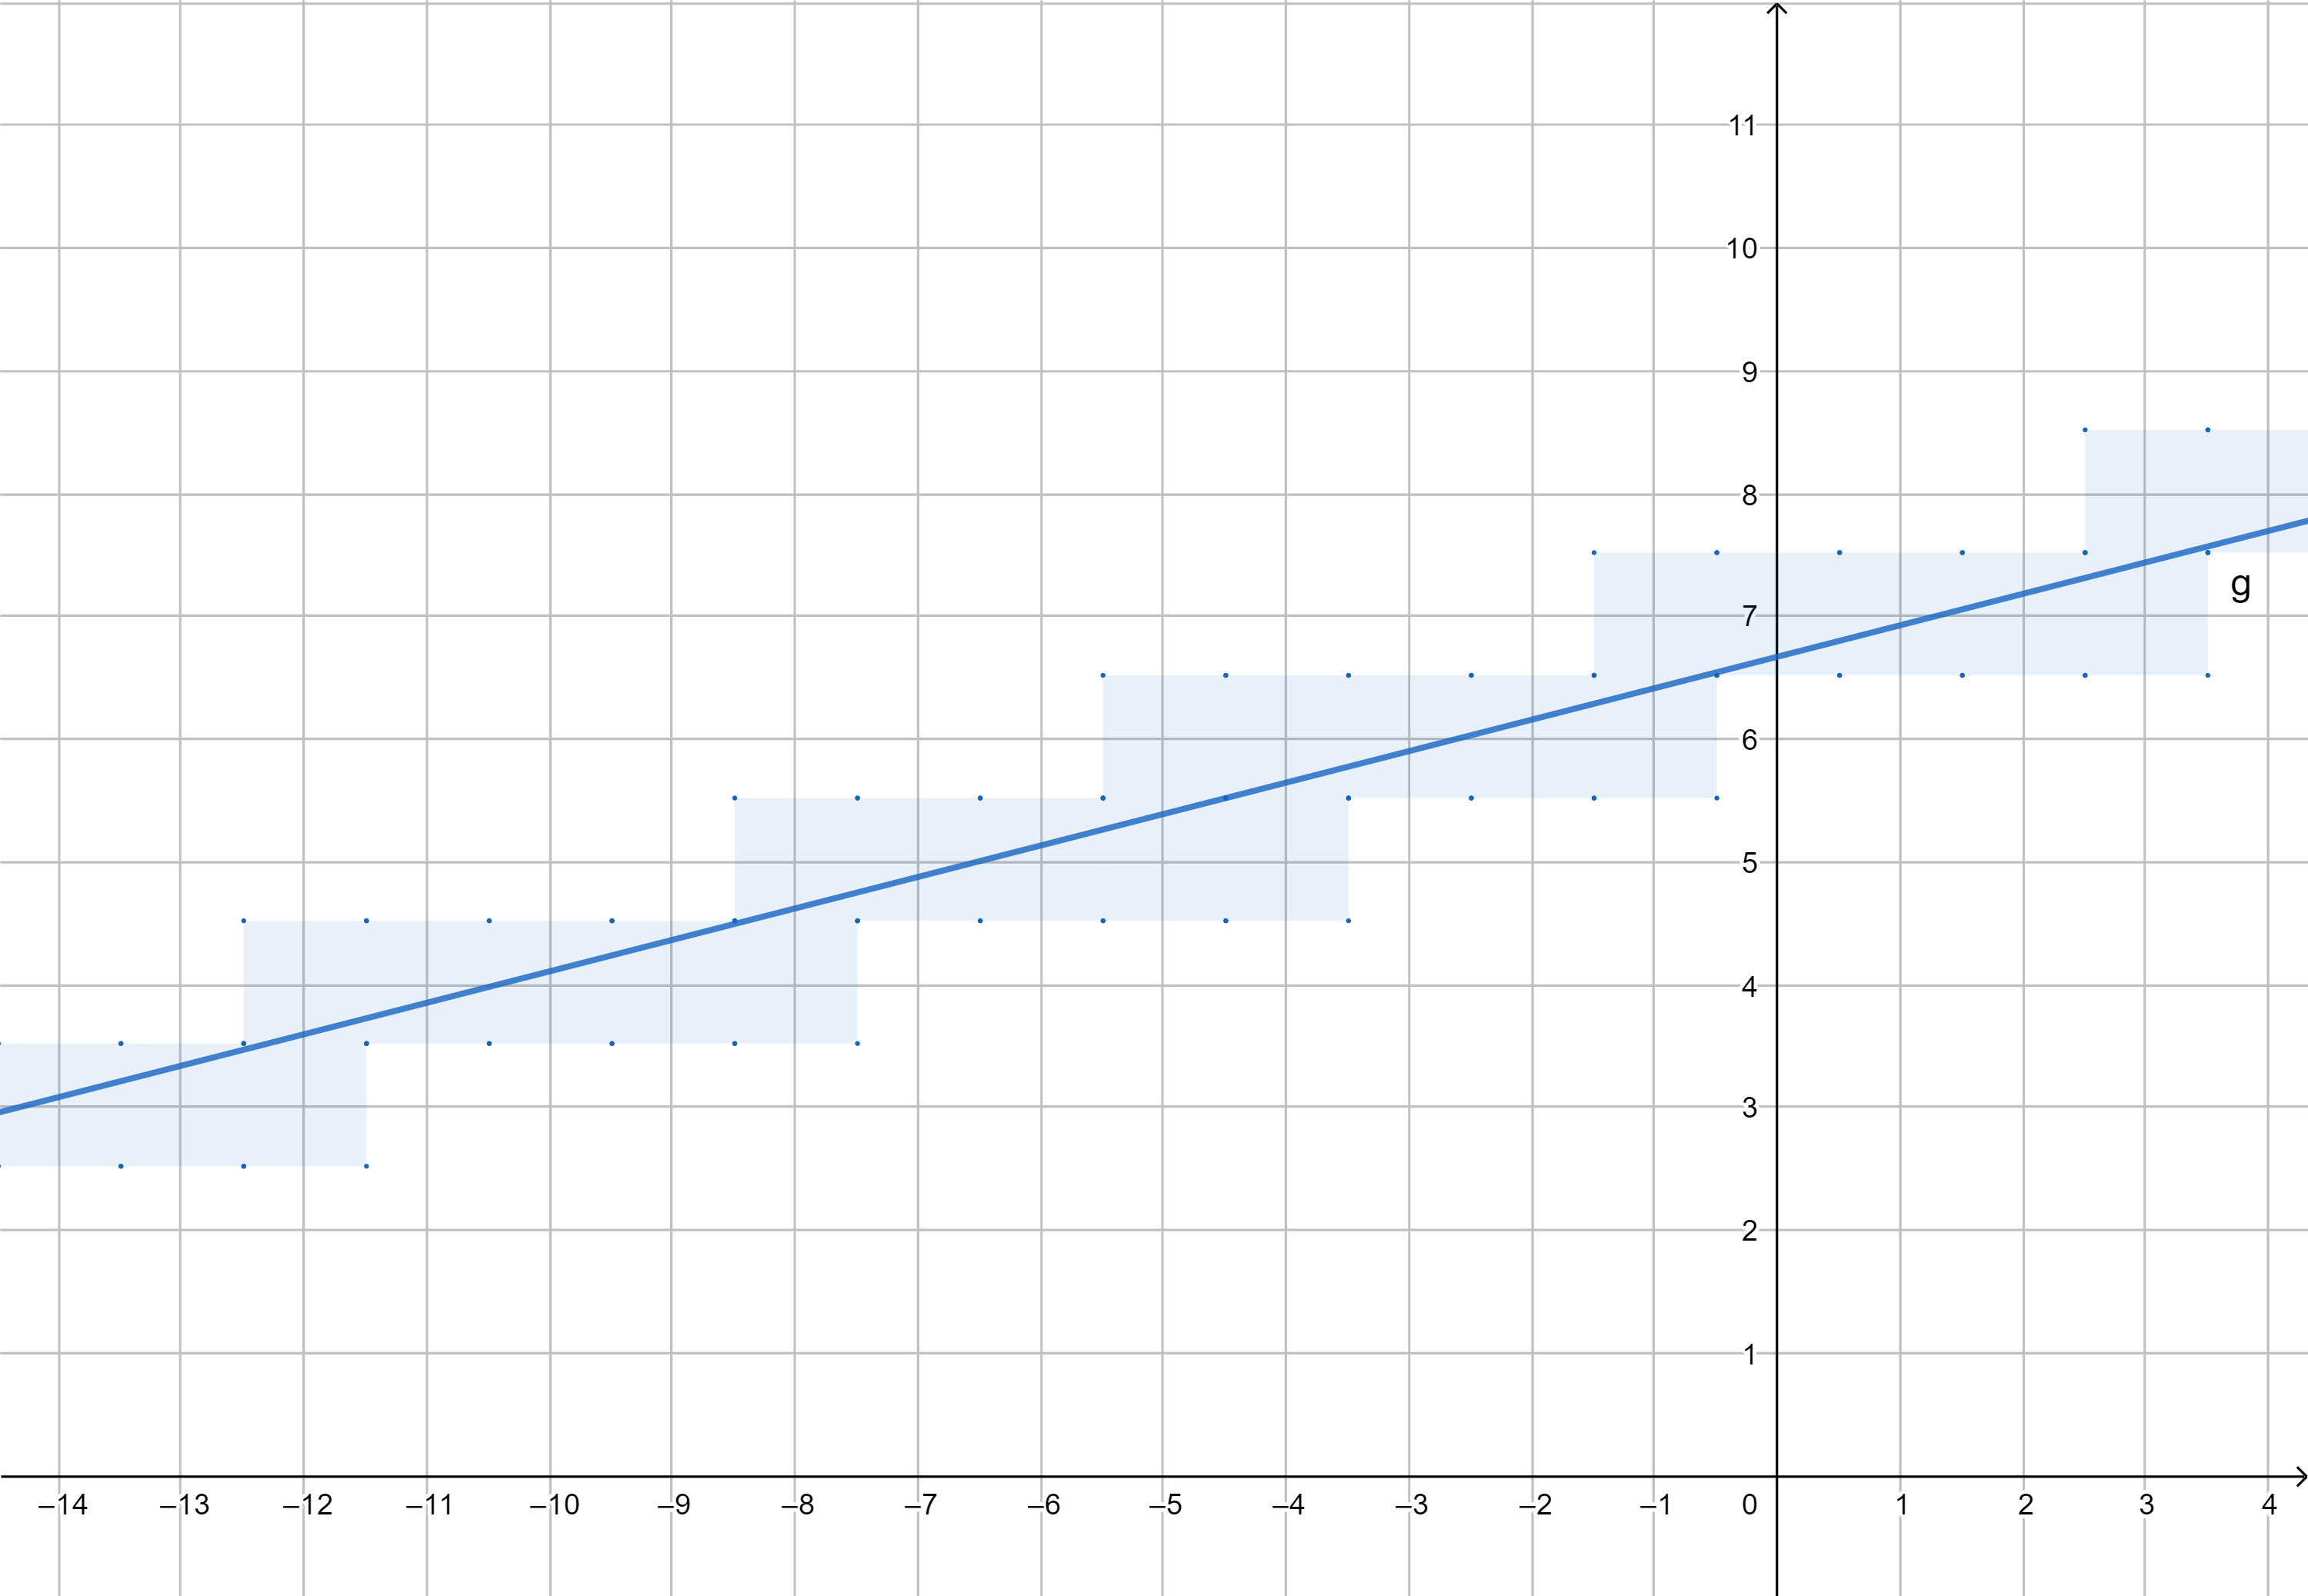
\includegraphics[height=10cm]{images/geogebra-images/line-hit-squares.png}
	\caption{$g$ hits squares around points} \label{linesquares}
	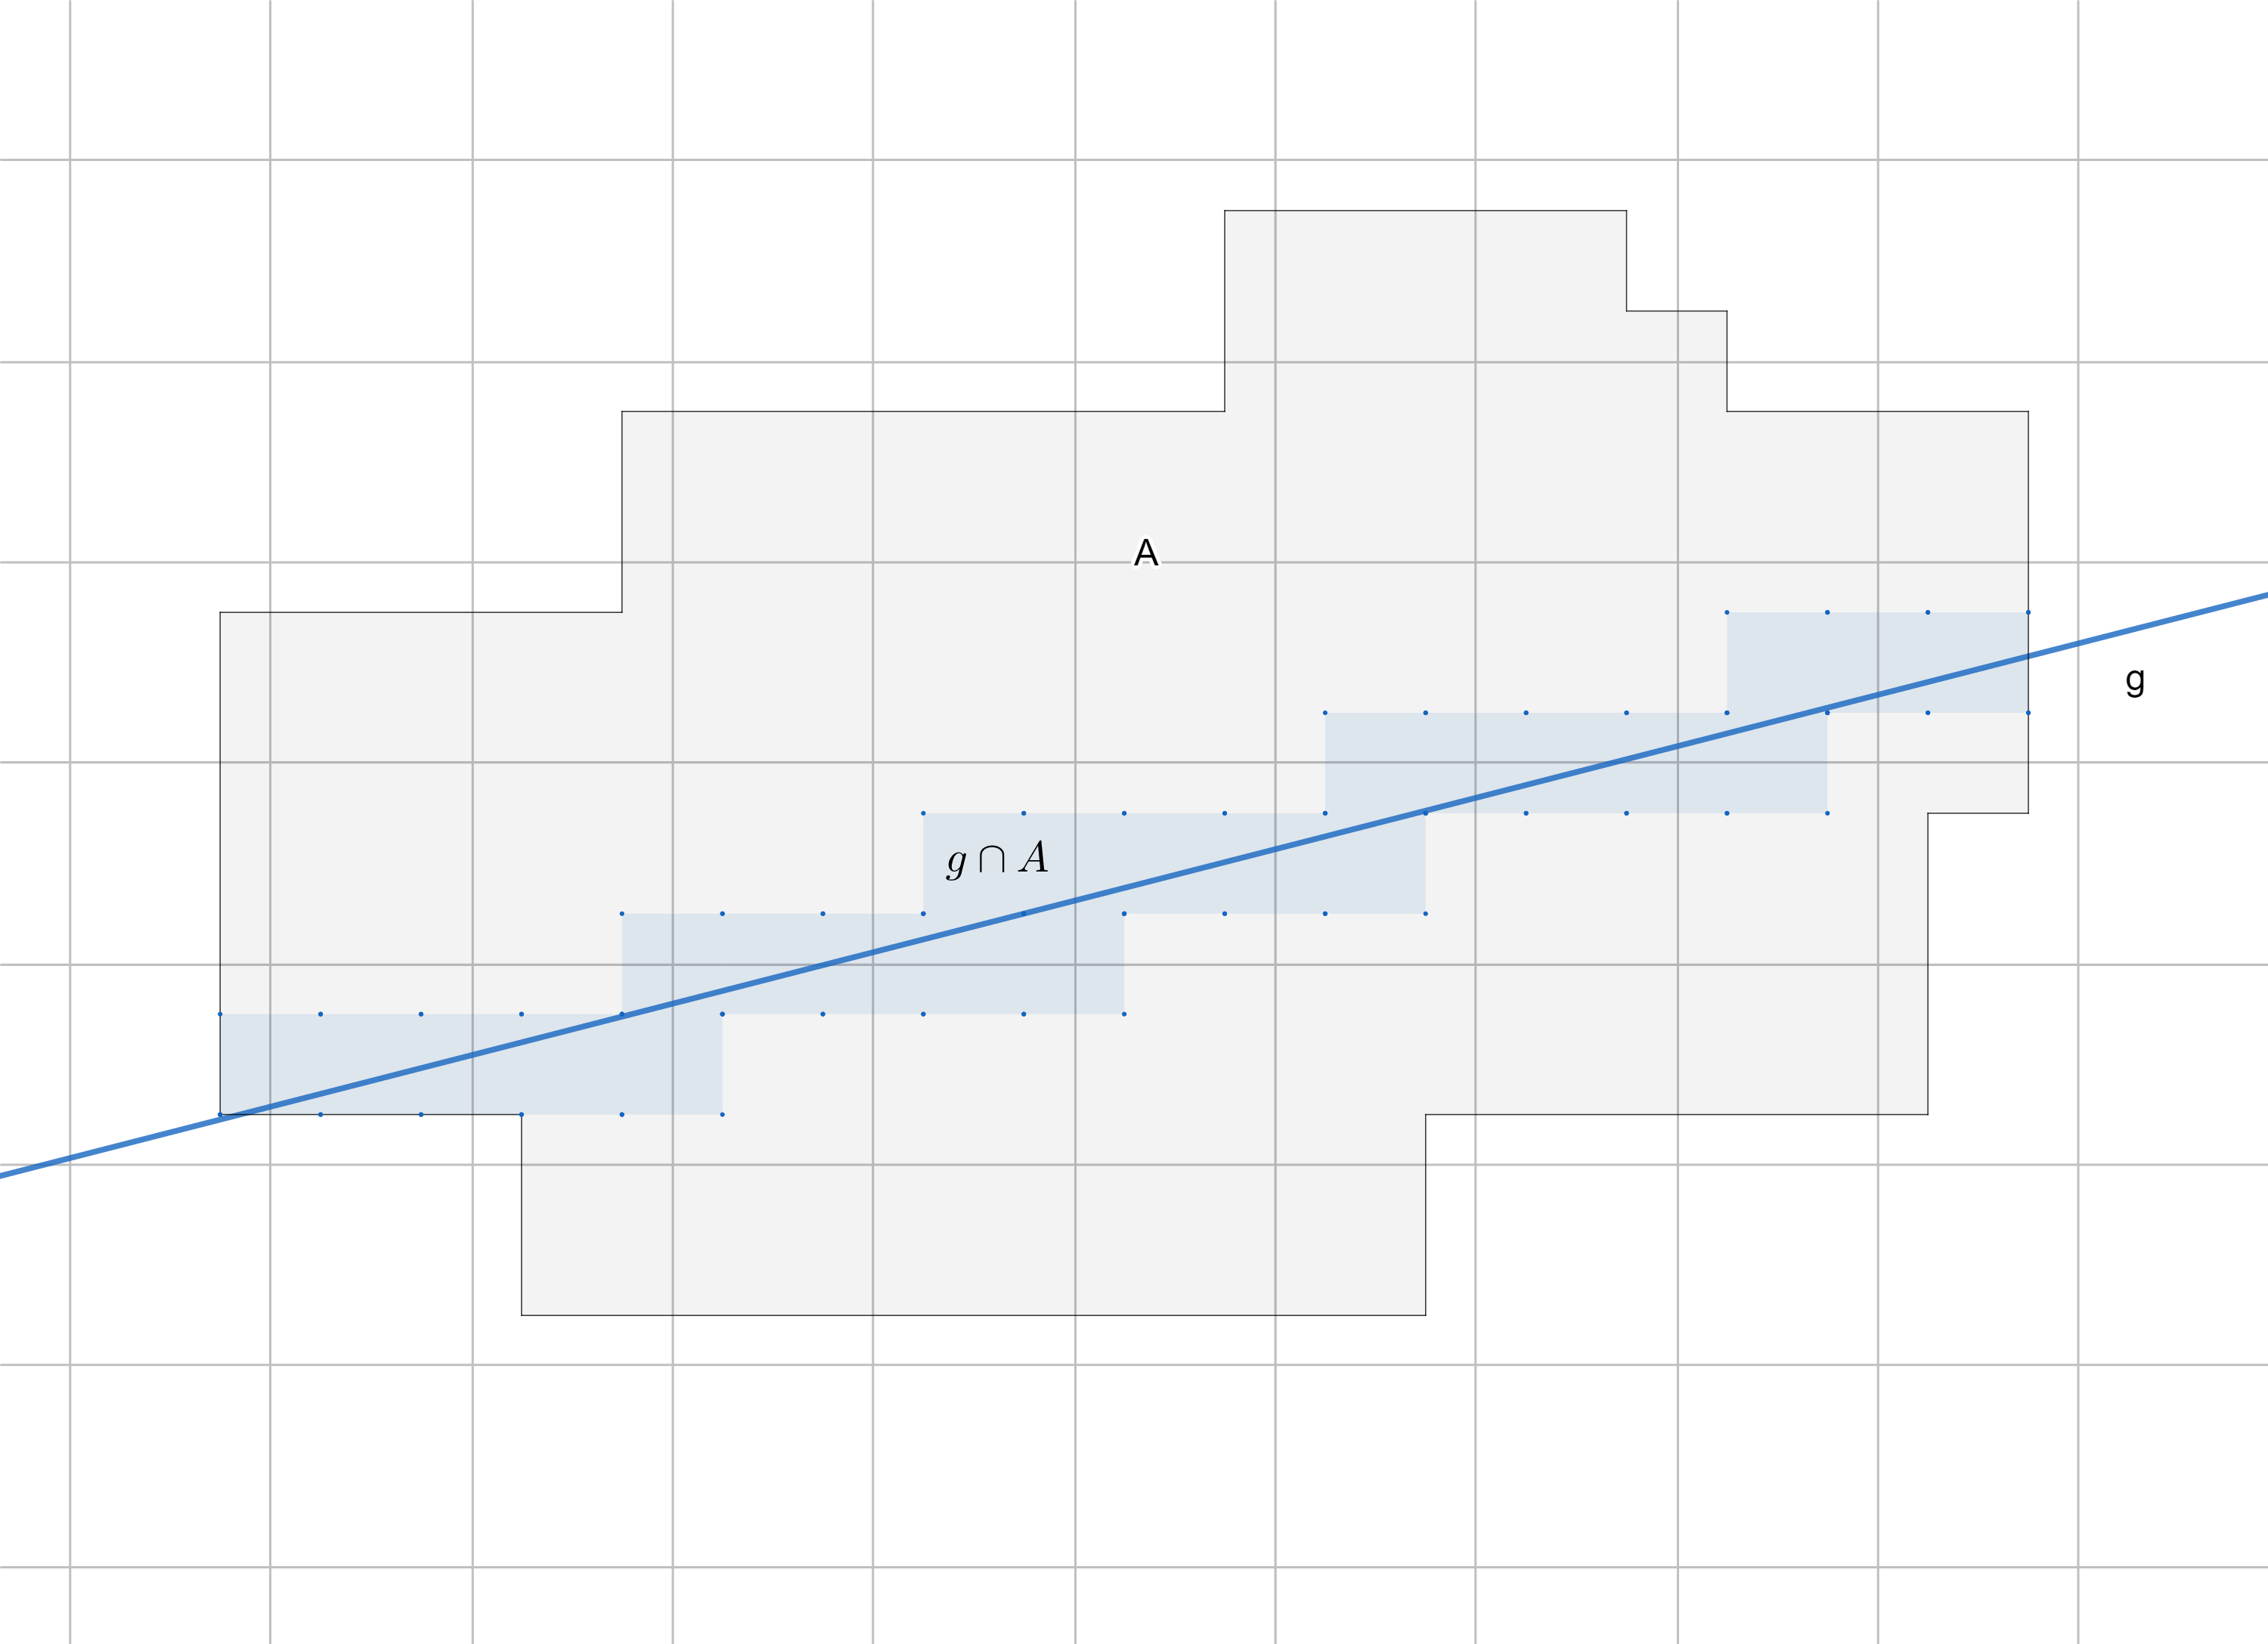
\includegraphics[height=10cm]{images/geogebra-images/line-hit-A.png}
	\caption{$g$ hits squares in $A$} \label{linesquaresA}
\end{figure}

\begin{definition} \label{ghitA}
	Let $g=g_{\alpha,p}\in \G$ and $A\in \mP_f$. We define 
	
	\begin{align*}
		g\cap A := \{ p\in A\ |\ g \text{ hits } p\}
	\end{align*}
	
	which is the subset of all points in $A$ which are hit by $g$ (see $\autoref{linesquaresA}$). For the following we suppose $g\cap A \neq \emptyset$. We will define a total ordered relation $\triangleleft$ on $g\cap A$ which shall be defined equivalently for all $g\in \G$ and $A\in\mP_f$ with $g\cap A \neq\emptyset$. We choose two points $x,y\in g\cap A$ and split the definition of the relation $\triangleleft$ into four cases, depending on whether the line $g$ goes from left-bottom to right-top, left-top to right-bottom, parallel to the $x$-axis and parallel to the $y$-axis. Denote the real part of $x$ with $\re(x)$ and the imaginary one with $\im(x)$. \\
	\\
	$\mathit{Case}\ 1:\quad g\ \text{ is parallel to the x-axis}\quad (\Leftrightarrow\quad \alpha = \frac{\pi}{2})$
	\begin{align*}
	x \triangleleft y \quad :\Leftrightarrow \quad \re(x) < \re(y)
	\end{align*}\\
	$\mathit{Case}\ 2:\quad g\ \text{ is parallel to the y-axis}\quad (\Leftrightarrow\quad \alpha = 0)$
	\begin{align*}
	x \triangleleft y \quad :\Leftrightarrow \quad \im(x) < \im(y)
	\end{align*}\\
	$\mathit{Case}\ 3:\quad g\ \text{ is going from left-bottom to right-top}\quad (\Leftrightarrow\quad \alpha\in (\frac{\pi}{2},\pi))$
	\begin{align*}
	x \triangleleft y \quad :\Leftrightarrow \quad
		\begin{cases}
			\re(x) < \re(y), & \text{ if } \re(x) \neq \re(y), \\
			\im(x) < \im(y), & \text{ if } \re(x) = \re(y).
		\end{cases}
	\end{align*}\\
	$\mathit{Case}\ 4:\quad g\ \text{ is going from left-top to right-bottom}\quad (\Leftrightarrow\quad \alpha\in (0,\frac{\pi}{2}))$
	\begin{align*}
	x \triangleleft y \quad :\Leftrightarrow \quad
	\begin{cases}
	\re(x) < \re(y), & \text{ if } \re(x) \neq \re(y), \\
	\im(x) > \im(y), & \text{ if } \re(x) = \re(y).
	\end{cases}
	\end{align*}\\
	It is easy to see that this relation on $g\cap A$ is well-defined. In the following we will prove that this relation is strictly and totally ordered. 
\end{definition}

\begin{lemma}
For a line $g=g_{\alpha,p}\in\G$ and $A\in \mP_f$ with $g\cap A\neq \emptyset$ the relation $\triangleleft$ on $g\cap A$ is totally ordered. 
	\begin{proof}
		We will only proove the case where $g$ is going from left-bottom to right-top, which is $\mathit{Case}\ 3$ of the definition. In this case we have $\alpha\in (\frac{\pi}{2},\pi)$. Note, that the proof for $\mathit{Case\ }4$ will work very similar and in the case of $g$ being parallel to one of the axes ($\mathit{Case\ }1$ or $2$), all properties for a totally ordered relation follow directly from the totally ordered relation $<$ on $\mathbb{R}$. So let $\alpha\in (\frac{\pi}{2},\pi)$. \\
		\\
		$\mathit{Antisymmetry:}$ For antisymmetry let $x \triangleleft y$ and $y \triangleleft x$. Suppose $\re(x)\neq \re(y)$, then $\re(x) < \re(y)$ and $\re(y) < \re(x)$, a contradiction because of the total order $<$ in $\mathbb{R}$. So $\re(x) = \re(y)$. But then we have $\im(x) < \im(y)$ and $\im(y) < \im(x)$ and therefore also $\im(x) = \im(y)$, hence $x=y$. \\
		\\
		$\mathit{Transitivity:}$ For transitivity let $x \triangleleft y$ and $y \triangleleft z$. We find four cases. In case $\re(x) \neq \re(y)$ and $\re(y) \neq \re(z)$ we get $\re(x) < \re(z)$ by transitivity of $<$, hence $x \triangleleft z$. In case $\re(x)\neq \re(y)$ and $\re(y) = \re(z)$ we get $\re(x) < \re(y) = \re(z)$, therefore $x \triangleleft z$. In case $\re(x) = \re(y)$ and $\re(y) \neq \re(z)$ we get $\re(x) = \re(y) < \re(z)$, similar as the last case. In the last case $\re(x) = \re(y) = \re(z)$ we get $\im(x) < \im(y)$ and $\im(y) < \im(z)$ and again by transitivity of $<$ we get $\im(x) < \im(z)$, hence $x \triangleleft z$ again. \\
		\\
		$\mathit{Connexity:}$ Connexity is given since for any two points $x,y\in g\cap A$ we have either $\re(x) \neq \re(y)$ or $\re(x) = \re(y)$ and therefore either $x\triangleleft y$ or $y\triangleleft x$.
	 
	\end{proof}
\end{lemma}

\begin{remark}
	The relation $\triangleleft$ on $g\cap A$ basically orders the hitting points of $g$ with $A$ from left to right (or bottom to top in case of a line parallel to the $y$-axis). This order allows us to identify the outermost hitting points which are the minimum and maximum of $g\cap A$ with respect to $\triangleleft$. To clarify, we define $\min (g\cap A) := x_0$ if and only if $x_0 \triangleleft x$ for all $x\in g\cap A,x\neq x_0$, analogously $\max(g\cap A)$. This means when moving on $g$ facing $A$ coming from infinity this order allows to know where in $A$ the line $g$ hits first when \glqq entering \grqq $A$ and where it hits last when \glqq leaving \grqq $A$. What we want to do next is to choose a line randomly out of all lines which hit the current cluster. This is isn`t an obvious task and we will have to develop a most fair underlying distribution on lines in the next section where we will touch basic aspects of Integral Geometry. 
\end{remark}






\subsection{Integral Geometry}

In the next section we want to define an approximation for External DLA. This approximation will be an incremental aggregation for which distribution definition we need some concepts and results from Integral Geometry which we will discuss and develop in this section. In the process we want to define we will want to choose a random line out of all lines which intersect with the current cluster of the aggregation. This random choosing is not obvious since most of the time the cluster will be strongly non symmetric and it is even less obvious how to actually get a realization of a random line when simulating with Python. In our case we are looking for a parametrisation of lines in the plane and a reasonable way of choosing parameters randomly. \\

We will introduce a possible solution for this problem first through the abstract and general concepts of integral geometry and later through a simple parametrisation for the case of lines in the plane which goes hand in hand with the general result.

\subsubsection{General results}

In the general context we are in $\R^d$ for $d\in \N$ and consider $q$-dimensional affine subspaces where $q\in \{0,\dots,d\}$, short $q$-flats in $\R^d$. The set of $q$-flats in $\R^d$ is denoted by $A(d,q)$. Later we will be interested in choosing random lines in the real plane (i.e. $1$-flats in $\R^2$). In order to get a probability measure on some set of $q$-flats, we first need a measure and a $\sigma$-algebra on $A(d,q)$ in total. 

\begin{definition}
	For $B\in \mathcal{B}^d$ define 
	\begin{flalign*}
		[B]_{d,q} := \{F\in A(d,q)\ |\ F\cap B \neq\emptyset\}.
	\end{flalign*}
	If the context is clear, we will only write $[B]$ instead of $[B]_{d,q}$. 
\end{definition}

\begin{definition}
	The $\sigma$-algebra $\mathcal{A}(d,q)$ on $A(d,q)$ is defined by
	\begin{flalign*}
		\mathcal{A}(d,q) := \sigma(\{ [K]\ |\ K\in \K^d\}).
	\end{flalign*} 
\end{definition}

\begin{theorem} \label{uniqmeas}
	On $A(d,q)$ there exists a unique $G_d$-invariant Radon measure $\mu_q$ such that
	\begin{flalign}
		\mu_q(A_{B_d(1,0)}) = \kappa_{d-q}, 
	\end{flalign}
	where $\kappa_n := \lambda_n(B_n(1,0))$ is the $n$-dimensional Lebesque meausure of the $n$-dimensional unit ball for $n\in \N$, and $\kappa_0:=1$.
\end{theorem}
\begin{proof}
	\cite{stoch1} Theorem 4.26 \\ \\ MAKE PROOF CLEARER
\end{proof}

\subsubsection{Construction in the plane: Isotropic lines}

For our special case we choose $d=2$ and $q=1$, thus lines in the plane. We denote this set of lines by $\G$. The following construction in this chapter is completely motivated by \cite{sackmann} 2.1.1. Firstly we propose a parametrisation of lines which works as follows. Every line can be uniquely determined by an angle $\alpha\in [0,\pi)$ and a real number $p\in \R$. Let $\langle\cdot,\cdot\rangle$ be the standard scalar product on $\R^2$, respectively used for values in $\C$ as we identify $\R^2$ with $\C$ as $\R$-vectorspaces. Let 
\begin{flalign*}
	e_\alpha := e^{\alpha i} = \cos(\alpha) + \sin(\alpha)i
\end{flalign*}
and 
\begin{flalign*}
	s_\alpha : = -\sin(\alpha) + \cos(\alpha)i
\end{flalign*}
be the unit vectors $1$ and $i$ rotated by $\alpha$ counterclockwise. Lets consider the representation $x = \langle x,e_\alpha\rangle e_\alpha + \langle x,s_\alpha\rangle s_\alpha$ for $x\in \C$. Since $e_\alpha$ and $s_\alpha$ form a base of $\C$ as a $\R$-vectorspace, the parameters $\langle x,e_\alpha\rangle$ and $\langle x, s_\alpha\rangle$ are unique for each $x$. It thus is easy to realize that $g_{\alpha,p} := \{x\in \C\ |\ \langle x,e_\alpha\rangle  = p\}$ defines a line (compare with $\autoref{lineparam}$) and that every line has a unique pair of $\alpha$ and $p$ for such a representation. In words, $g_{\alpha,p}$ contains all points which have length $p$ in direction of $e_\alpha$. With $\Phi := [0,\pi) \times \R$ this naturally defines a bijection
\begin{flalign*}
	\chi: \Phi \to \G, \quad (\alpha,p) \mapsto g_{\alpha,p}. 
\end{flalign*}
\\
\begin{figure}
	\centering
	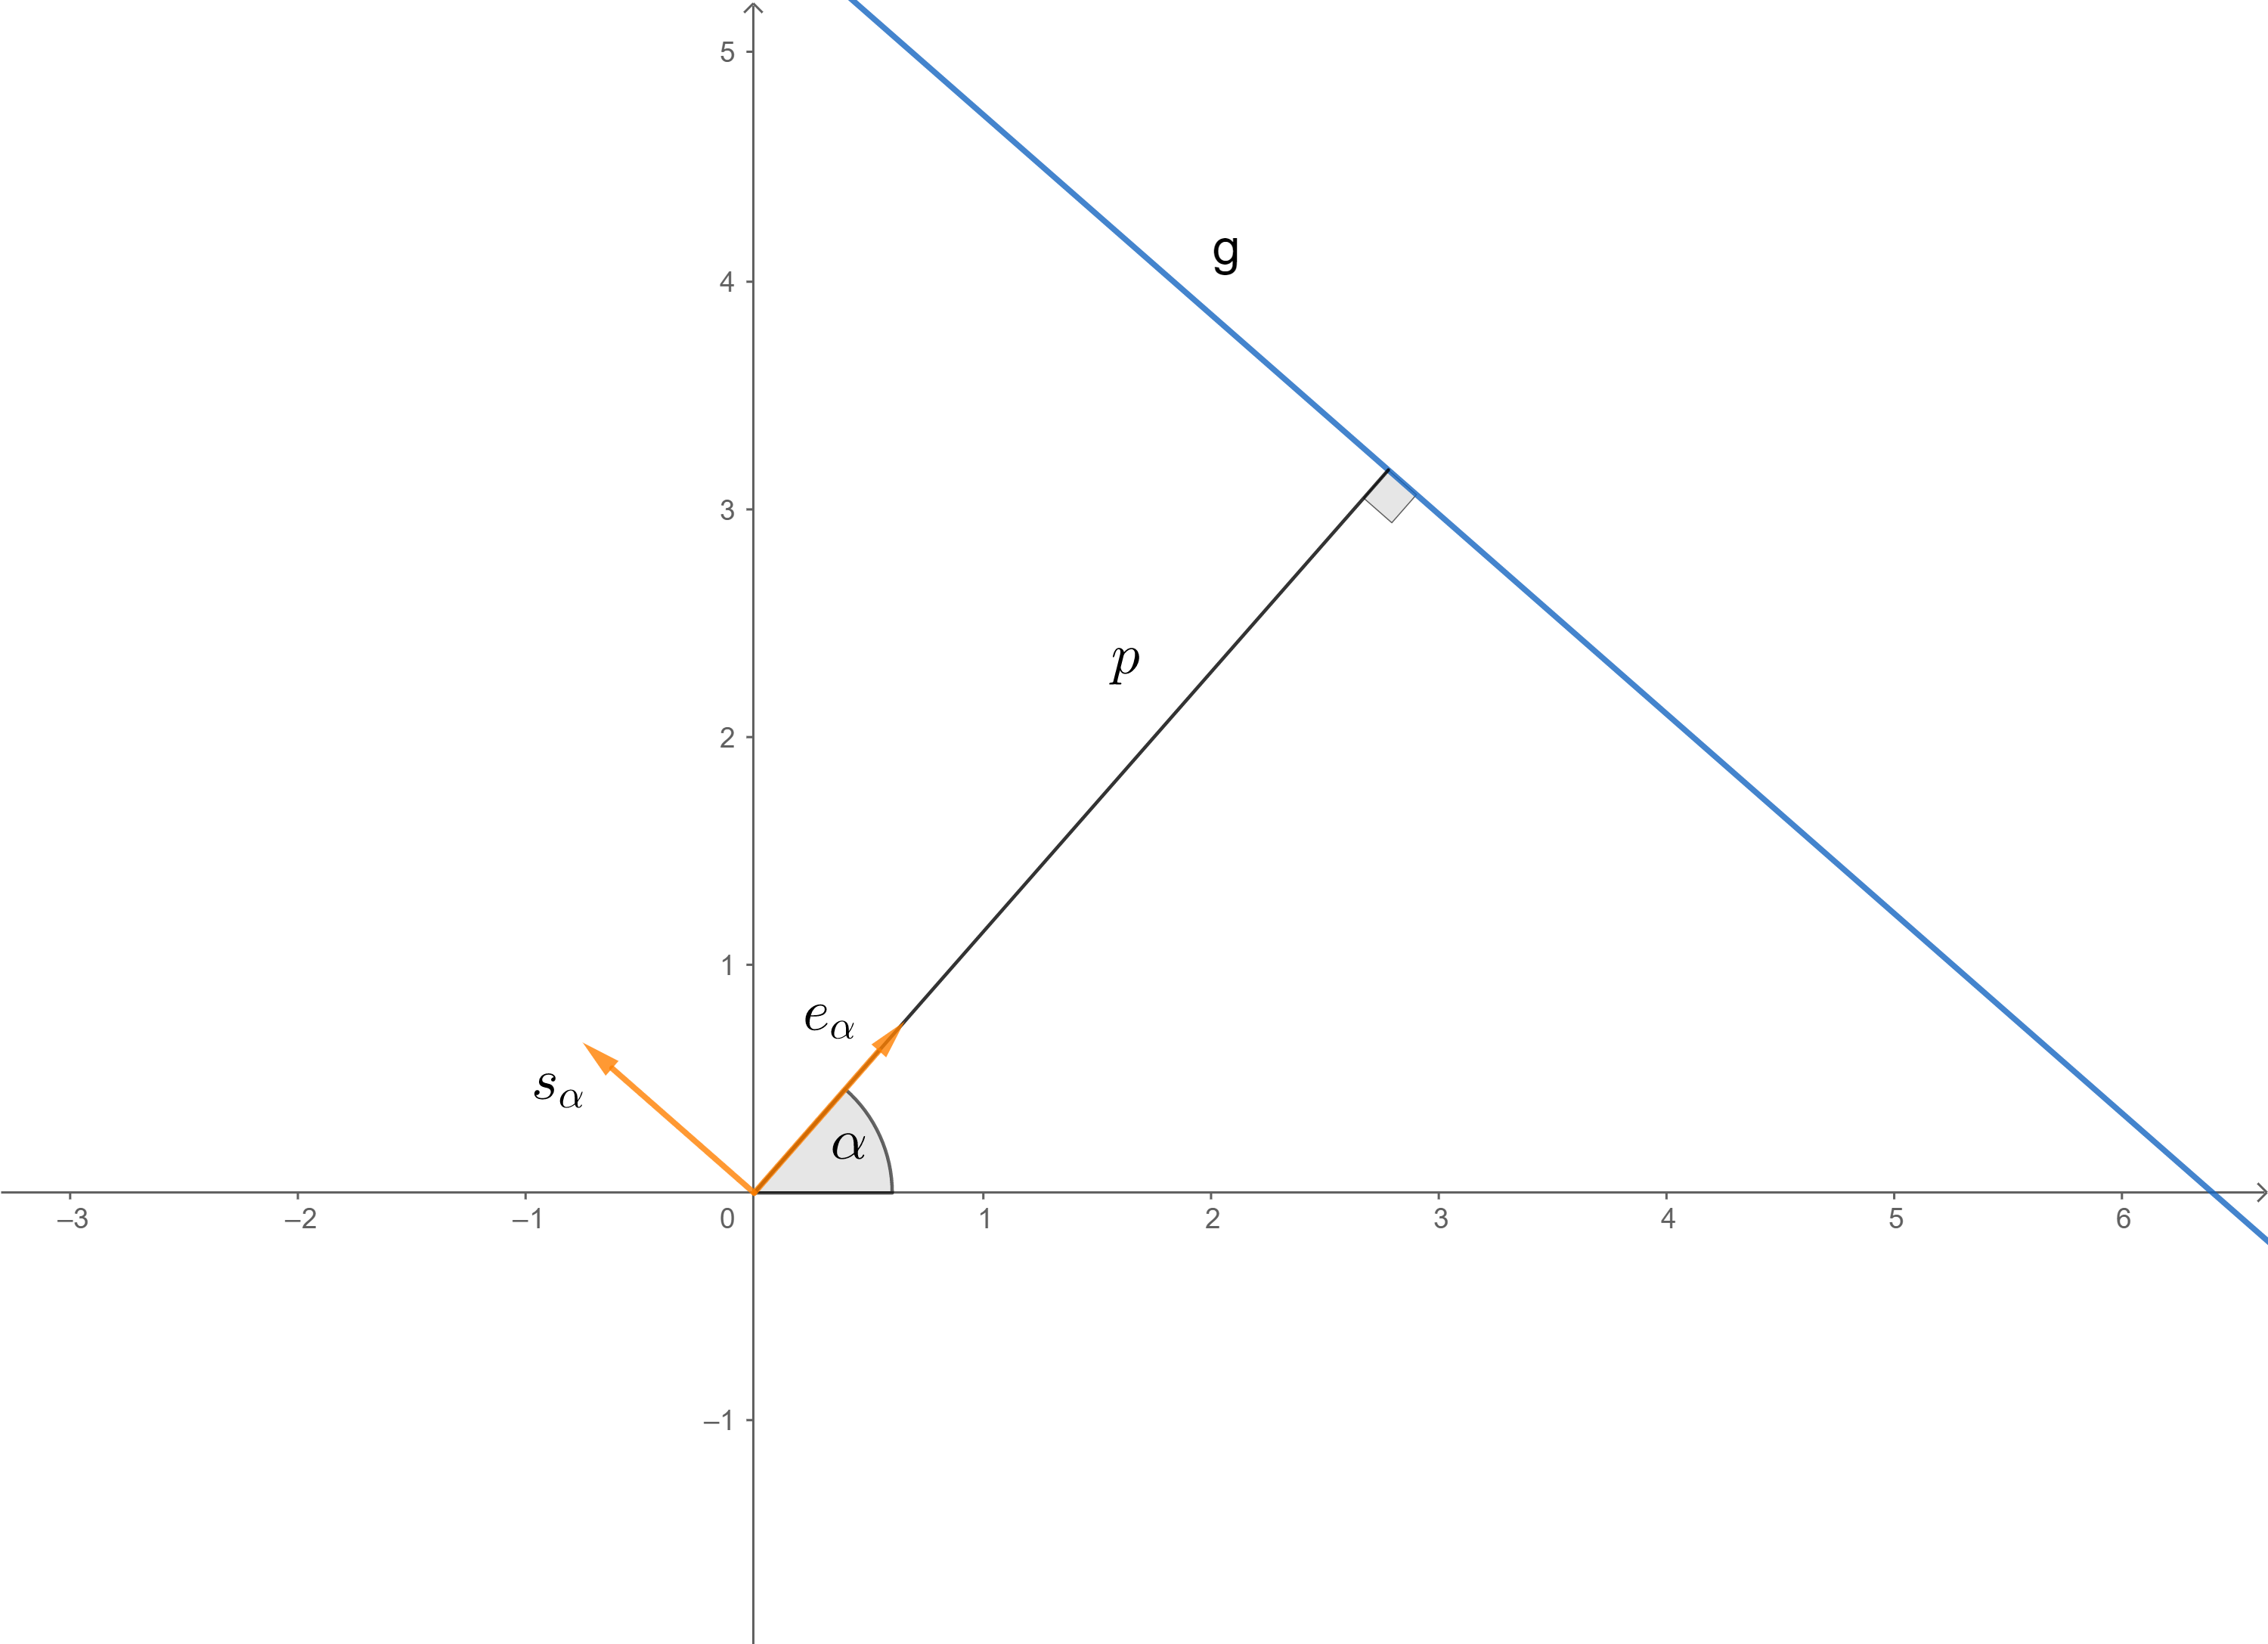
\includegraphics[height=10cm]{images/geogebra-images/line-param.png}
	\caption{Line parameters $\alpha$ and $p$} \label{lineparam}
\end{figure}
\\


We take the subspace Borel-$\sigma$-algebra $\mathcal{B}_\Phi:= \mathcal{B}^2 \cap \Phi$ on $\Phi$ and define the $\sigma$-algebra $\GG$ on $\G$ by $\GG := \chi(\mathcal{B}_\Phi)$. This works well since $\chi$ is a bijection. We want to show in the following that this way of defining a $\sigma$-algebra on $\G$ makes sense as it is indeed equivalent to the general context as defined above. To do that it is convenient to use a special generator set for the Borel-$\sigma$-algebra $\mathcal{B}_\Phi$. 

\begin{lemma} \label{generators}
	Define 
	\begin{flalign*}
		\mathcal{R}_+ := \{[\alpha,\beta]\times (0,b]\ |\ 0\leq \alpha<\beta<\pi, b \geq 0\}, 
	\end{flalign*}
	\begin{flalign*}
		\mathcal{R}_- := \{[\alpha,\beta]\times [b,0)\ |\ 0\leq \alpha<\beta<\pi, b\leq 0\},
	\end{flalign*}
	\begin{flalign*}
		\mathcal{R}_0 := \{[\alpha,\beta]\times \{0\}\ |\ 0\leq \alpha<\beta<\pi\},
	\end{flalign*}
	and
	\begin{flalign*}
		\mathcal{R} := \mathcal{R}_+ \cup \mathcal{R}_- \cup \mathcal{R}_0.
	\end{flalign*}
	Then $\sigma(\mathcal{R}) = \mathcal{B}_\Phi$.
\end{lemma}
\begin{proof}
	We show that $\sigma(\mathcal{R})$ contains all rectangles in $\Phi$ of the form $[\alpha,\beta]\times (a,b]$ with $a,b>0$, $[\alpha,\beta]\times [a,b)$ with $a,b<0$ and $[\alpha,\beta]\times [a,b]$ with $0\in [a,b]$. First let $a,b>0$ and $R=[\alpha,\beta]\times (a,b]$, then 
	\begin{flalign*}
		R = ([\alpha,\beta] \times (0,b]) \setminus ([\alpha,\beta] \times (0,a])
	\end{flalign*}
	and therefore $R\in \sigma(\mathcal{R}_+)\subset\sigma(\mathcal{R})$. Similarly it works if $a,b<0$. If $0\in[a,b]$ then we can write $R = [\alpha,\beta]\times [a,b]$ with three components $R = [\alpha,\beta] \times [a,0) \cup [\alpha,\beta] \times \{0\} \cup [\alpha,\beta] \times (0,b]$ which lie in $\mathcal{R}_-, \mathcal{R}_0$ and $\mathcal{R}_+$ respectively. Therefore $R\in \sigma(\mathcal{R})$ as well. By measure theory the above described rectangles form a generator set of $\mathcal{B}_\Phi$, which completes the proof. 
\end{proof}

\begin{lemma}
	We have $\mathcal{A}(2,1) = \GG$. 
\end{lemma}
\begin{proof}
	We will consider generators of these $\sigma$-algebras. By Lemma $\autoref{generators}$ we know that $\sigma(\mathcal{R}) = \mathcal{B}_\Phi$ and since $\chi$ is a bijection, we have $\chi(\sigma (\mathcal{R})) = \sigma (\chi(\mathcal{R}))$ and finally $\GG = \sigma(\chi(\mathcal{R}))$. For $\tilde A := \{[K]\ |\ K\in \K^2\}$ we have by definition $\mathcal{A}(2,1) = \sigma(\tilde A)$. \\
	%
	\\ \indent $\subset$: Let $K\in\K^2$. We will show that $\chi^{-1}([K])$ is a closed set in $\Phi$. If that is the case we have $\chi^{-1}([K])\in\mathcal{B}_\Phi$, therefore $[K] \in\chi(\mathcal{B}_\Phi) = \GG$ and finally $\mathcal{A}(2,1) = \sigma(\tilde A)\subset\GG$. To show that $\chi^{-1}([K])$ is closed let $(\alpha_0,p_0)\in \Phi\setminus \chi^{-1}([K])$. Then $\chi(\alpha_0,p_0) \notin [K]$ and therefore $\chi(\alpha_0,p_0) \cap K= \emptyset$. Since $K$ is closed we can find small values $\tilde\alpha,\tilde p > 0$ such that $\chi(\alpha,p) \cap K = \emptyset$ for all $(\alpha,p)\in [\alpha_0, \alpha_0 + \tilde\alpha] \times [p_0, p_0 + \tilde p] =: R$. Hence we have $ R\subset \Phi \setminus \chi^{-1}([K])$, so $\Phi \setminus \chi^{-1}([K])$ is open. Hence $\chi^{-1}([K])$ is closed. \\
	%
	\\ \indent $\supset$: For this inclusion we will show that $\chi(R)\in\mathcal{A}(2,1)$ for all $R\in\mathcal{R}$. First let $R = [\alpha,\beta]\times(0,b]\in\mathcal{R}_+$ for some $b>0$. Define 
	\begin{flalign*}
		S:= \{pe_\gamma \in \C\ |\ (\gamma,p)\in R\}
	\end{flalign*}
	Furthermore for $n\in \N$ define 
	\begin{flalign*}
		A_n := \{tns_\beta\ |\ t\in [0,1]\} \text{ and } B_n := \{-tns_\alpha\ |\ t\in [0,1]\},
	\end{flalign*}
	the segments from $0$ to $ns_\beta$ and $0$ to $-ns_\alpha$ ($\autoref{circleS}$). We will show now that 
	\begin{flalign*}
		\chi(R) = [\bar S] \setminus (\bigcup_{n\in\N} [A_n] \cup \bigcup_{n\in\N} [B_n]) =: \tilde S,  
	\end{flalign*}
	
	\begin{figure}
		\centering
		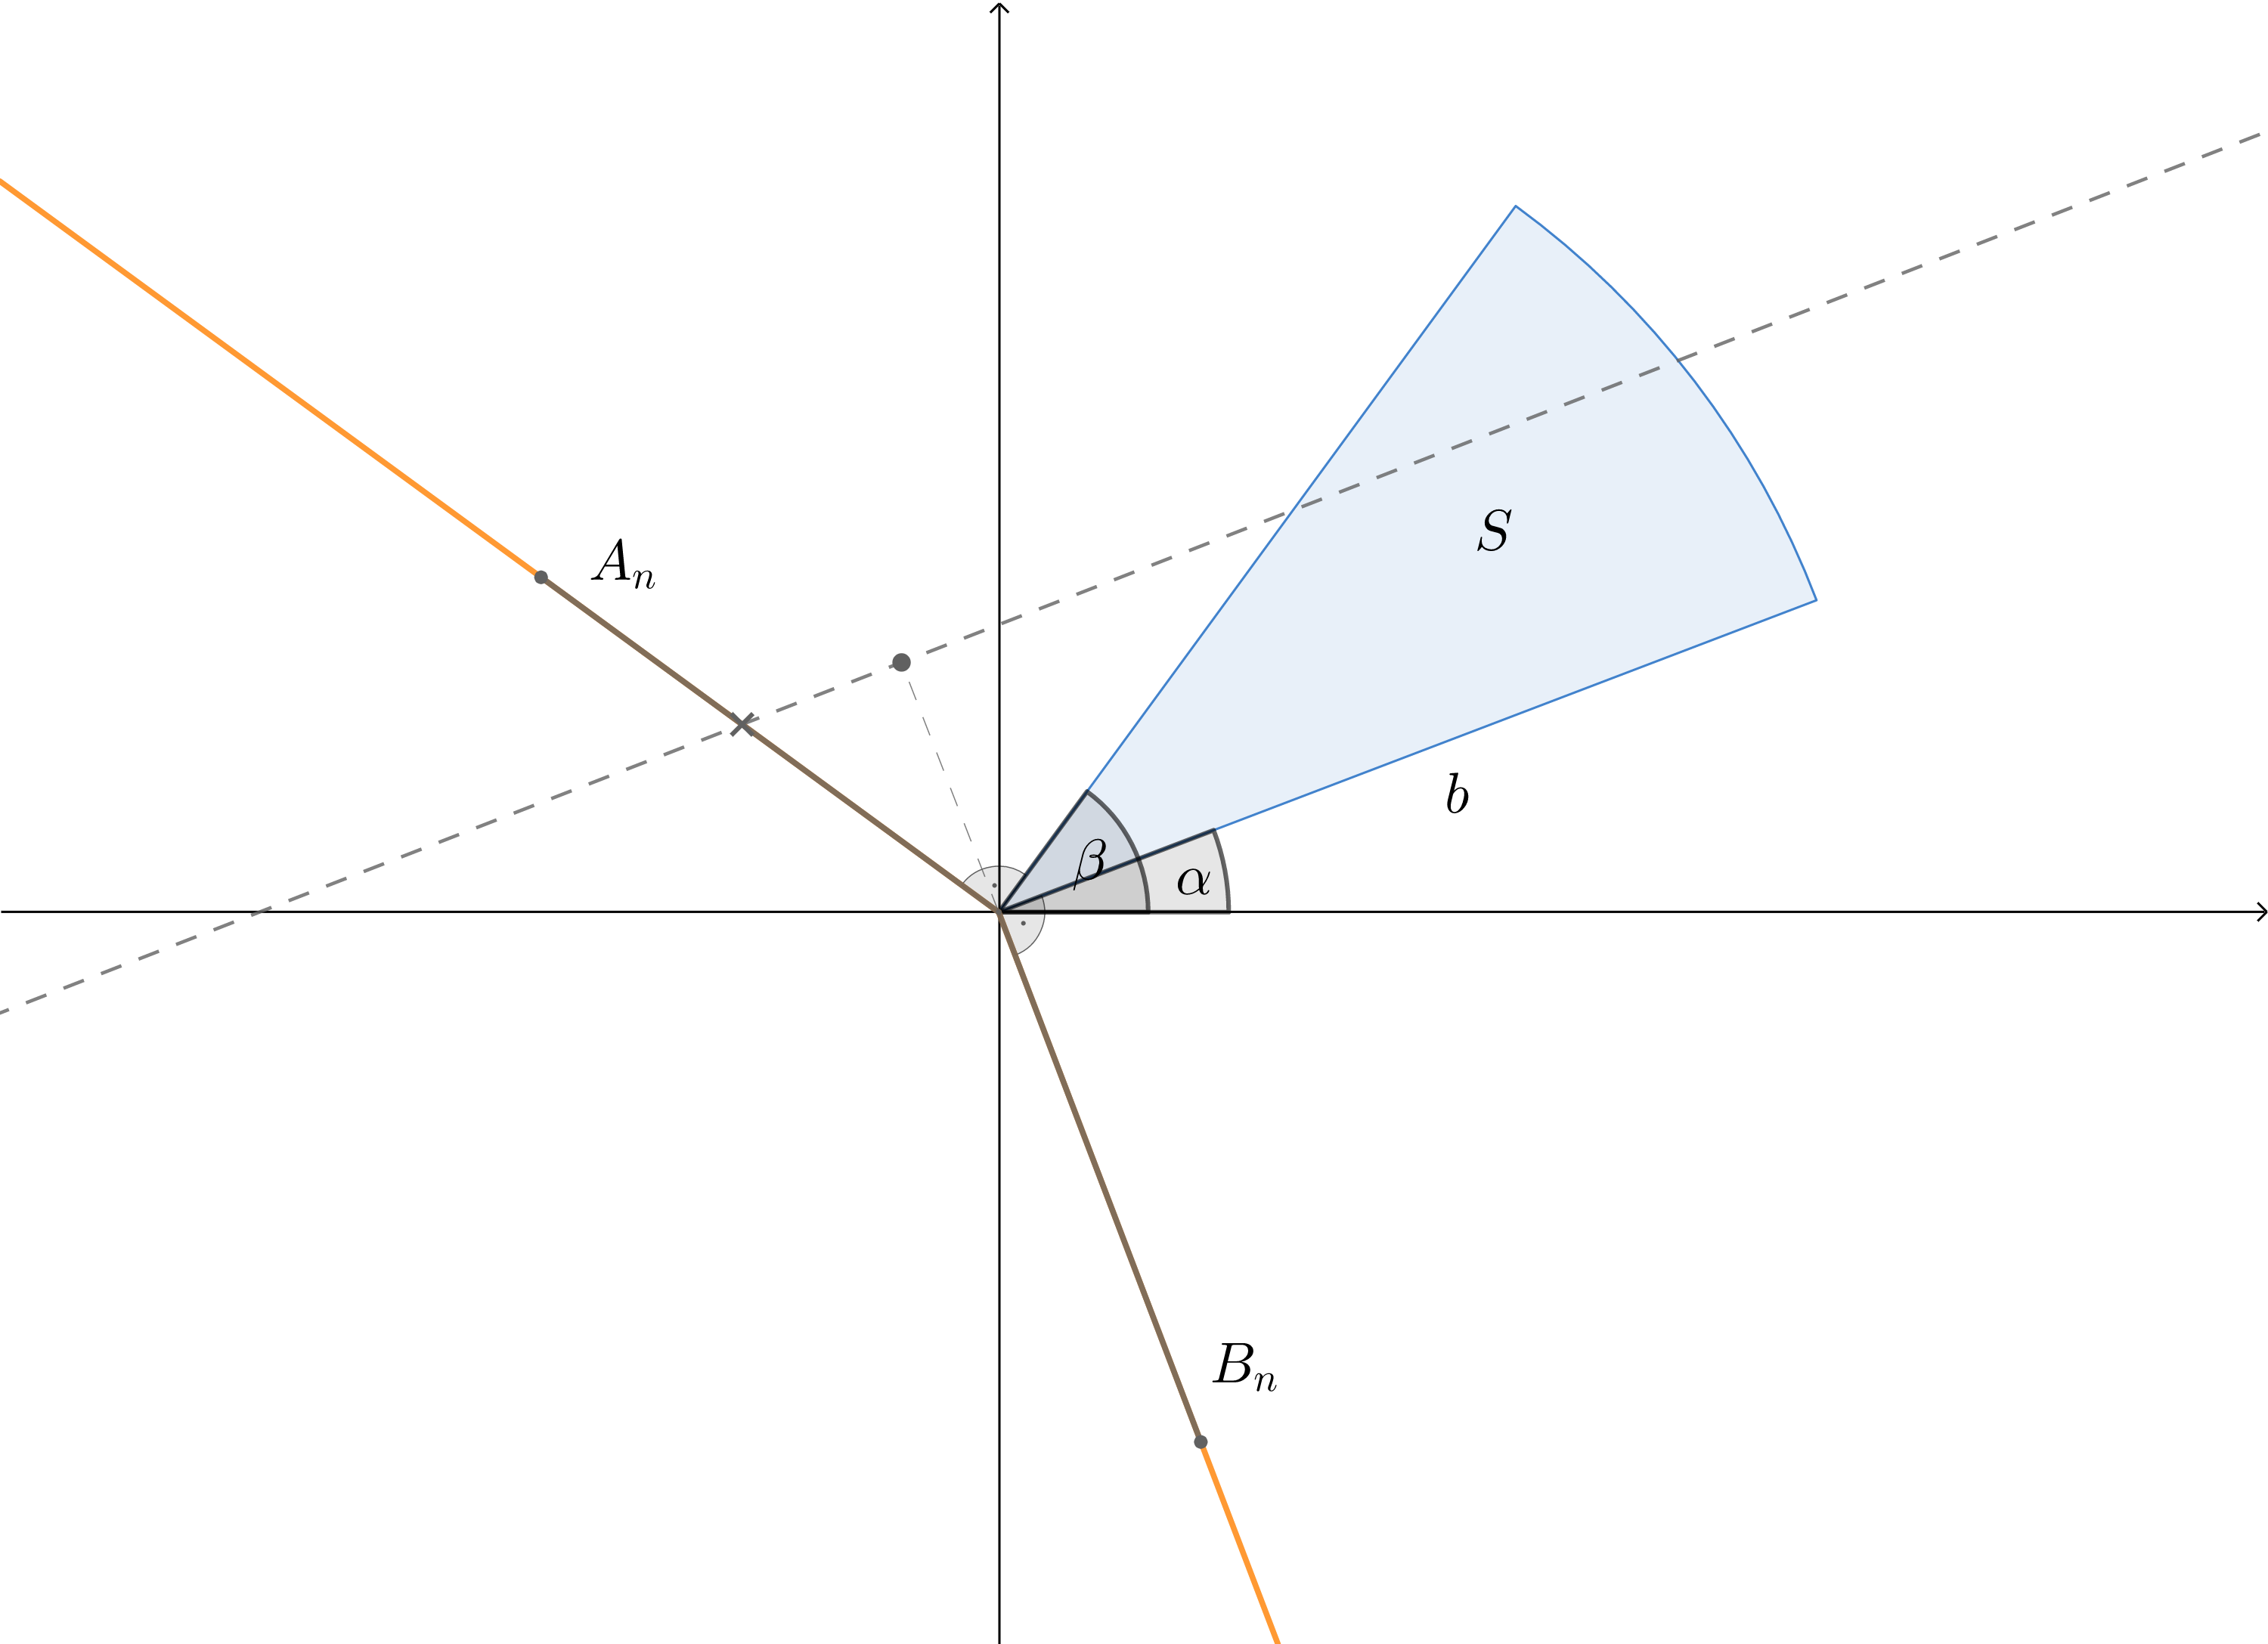
\includegraphics[height=10cm]{images/geogebra-images/circle-part-S.png}
		\caption{$S$ and the sets $A_n$ and $B_n$} \label{circleS}
	\end{figure}
	
	where $\bar S$ is the closure of $S$ (note that $\bar S = S\ \cup\ \{0\}$). Let $(\gamma,p)\in R$. Then $pe_\gamma\in \chi(\gamma,p)\cap S$ and therefore $\chi(\gamma,p)\in [\bar S]$. Assume that there exits an $n\in\N$ such that $\chi(\gamma,p)\cap A_n \neq \emptyset$. Then $\beta + \frac{\pi}{2} - \gamma < \frac{\pi}{2}$, hence $\beta < \gamma$, a contradiction. Similarly argument for any $B_n$, so we finally have $\chi(\gamma,p) \notin [A_n]$ and $\chi(\gamma,p) \notin [B_n]$ for any $n\in \N$. Hence $\chi(\gamma,p)\in\tilde S$ and therefore $\chi(R)\subset \tilde S$. \\
	\\
	Now let $(\gamma,p)\in\Phi$ such that $\chi(\gamma,p)\in \tilde S$. Assume that $\gamma\notin[\alpha,\beta]$ then with a similar argument as in the first inclusion it is easy to see that there must be an $n\in\N$ such that $\chi(\gamma,p)\cap A_n\neq \emptyset$ or $\chi(\gamma,p)\cap B_n\neq \emptyset$, a contradiction. Therefore $\gamma\in[\alpha,\beta]$. Now assume $p\notin (0,b]$. If $p>b$ then $\chi(\gamma,b)\cap B_b = \emptyset$ and since $\bar S\subset B_b$ it is $\chi(\gamma,p)\notin [\bar S]$, a contradiction. If $p<0$ then, since the angle between the segments $A_n$ and $B_n$ opposite of $S$ is strictly smaller than $\pi$, $\chi(\gamma,p)$ must intersect with $A_n$ or $B_n$ for some $n\in\N$, again a contradiction. Note that $p\neq 0$ since $[\{0\}] \subset [A_1]$. Thus we have $p\in(0,b]$. Therefore we have $(\gamma,p)\in R$ and finally $\tilde S\subset \chi(R)$. \\
	\\
	It is left to show that $\tilde S\in \mathcal{A}(2,1)$. All the segments $A_n$ and $B_n$ are compact and convex for all $n\in\N$, and since $S$ is bounded and convex as a circle segment with angle smaller than $\pi$, $\bar S$ is compact and convex. Finally $\tilde S\in \mathcal{A}(2,1)$. \\
	\\
	In total we get $\mathcal{R}_+\subset \mathcal{A}(2,1)$. $\mathcal{R}_-\subset \mathcal{A}(2,1)$ can be shown analogously. So for the last case let $R = [\alpha,\beta] \times \{0\}\in \mathcal{R}_0$. Define the line segment
	\begin{flalign*}
		T := \{(1-t)s_\alpha + ts_\beta\ |\ t\in [0,1]\}. 
	\end{flalign*}
	Then $[\{0\}] \cap [T] \in \mathcal{A}(2,1)$. We show that $\chi(R) = [\{0\}] \cap [T]$. Let $(\gamma,0)\in R$. Then $\chi(\gamma,0)$ contains $0$ and since $\gamma$ is in between $\alpha$ and $\beta$, $\chi(\gamma,0)$ must intersect with $T$ ($\autoref{T}$). For the other inclusion let $(\gamma,p)\in\Phi$ such that $\chi(\gamma,p)\in [\{0\}] \cap [T]$. Since $0\in \chi(\gamma,p)$ it must be $p=0$ and since it intersects with $T$ its angle must lay in between $\alpha$ and $\beta$. All in all this completes the proof. 
\end{proof}

\begin{figure}
	\centering
	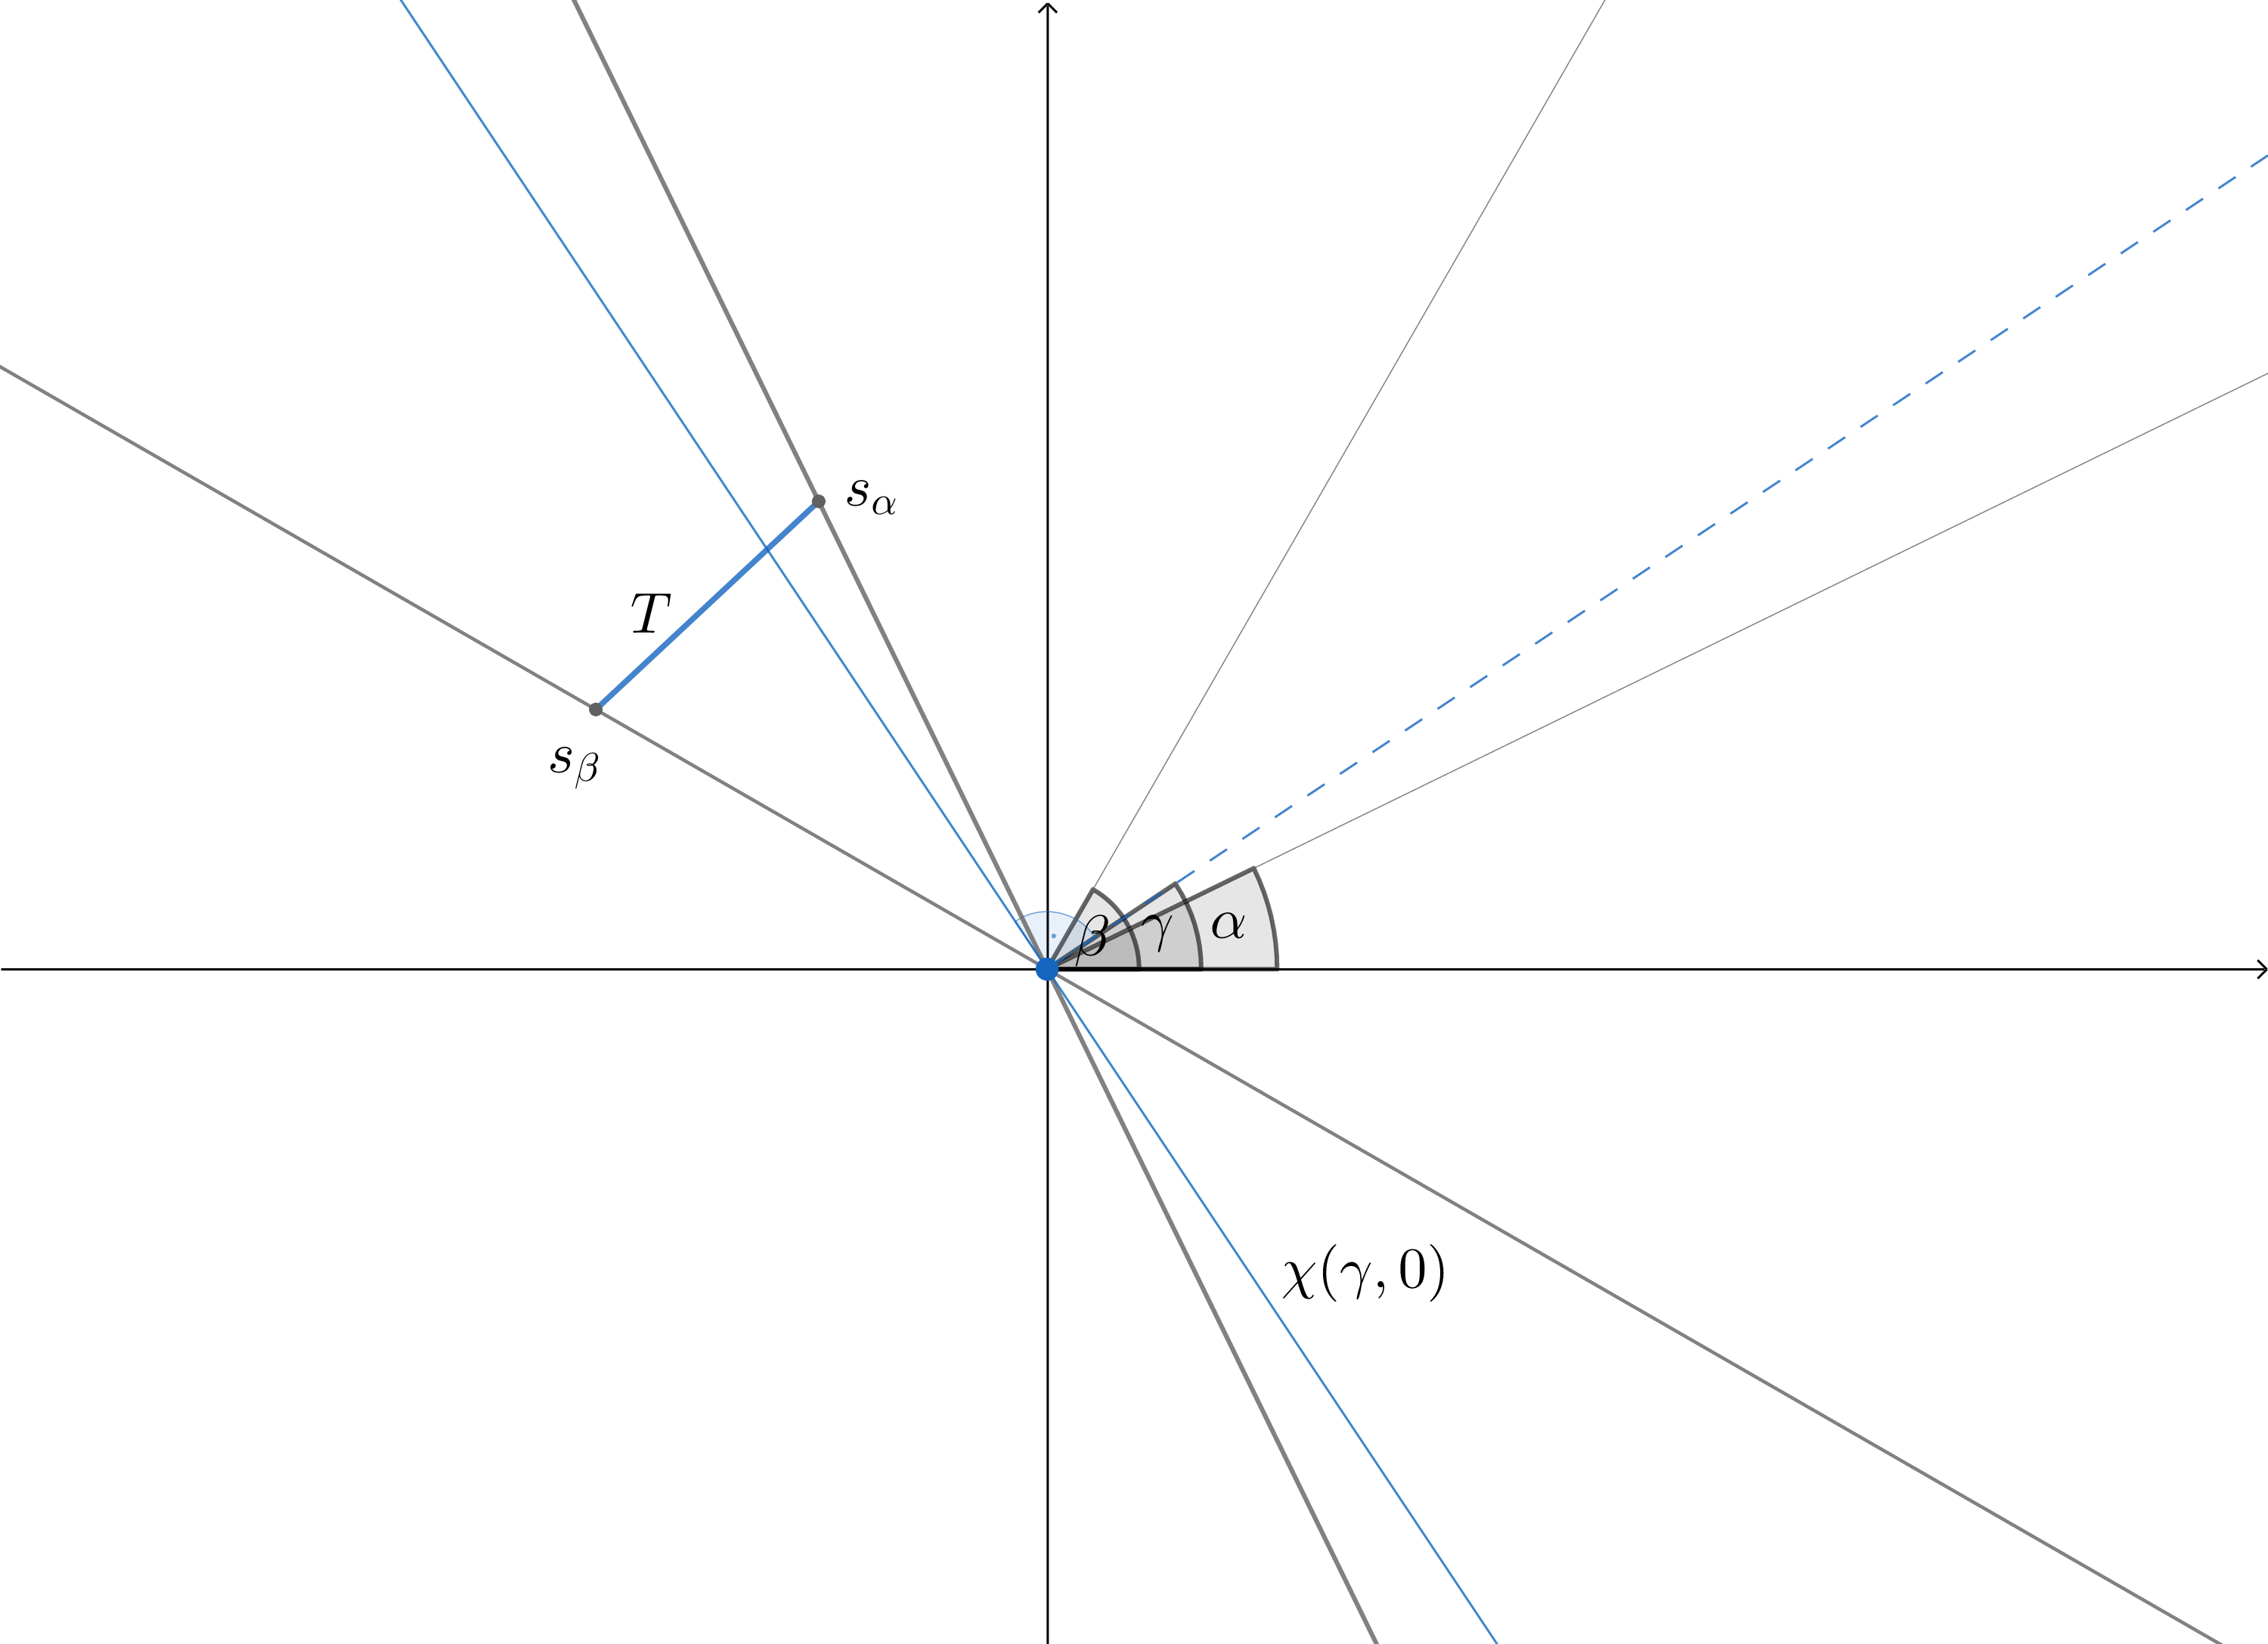
\includegraphics[height=10cm]{images/geogebra-images/T.png}
	\caption{Line in $[\{0\}] \cap [T]$} \label{T}
\end{figure}


\begin{definition}
	A $\mathcal{F}$-$\GG$-measurable function $g:\Omega \to \G$ is called a $\mathit{random\ line}$.  
\end{definition}

\begin{definition}
	We define the measure $\mu := {\lambda_2}_{|\Phi} \circ \chi^{-1}$ on $(\G,\GG)$ where ${\lambda_2}_{|\Phi}$ is the $2$-dimensional Lebesgue measure restricted to $\Phi$. We say a measure $\nu$ on $(\G,\GG)$ is locally finite if for any $K\in \K^2$ we have $\nu([K])<\infty$. 
\end{definition}

\begin{lemma}
	$\mu$ is locally finite and $G_2$-invariant. 
\end{lemma}
\begin{proof}
	Let $K\in \K^2$ and since $K$ is compact choose $r> 0$ such that $K\subset B_r$. Then we have $[K]\subset A_{B_r}$ and
	\begin{flalign*}
		\mu([K]) \leq \mu(A_{B_r}) = {\lambda_2}_{|\Phi} (\chi^{-1}(A_{B_r})) = {\lambda_2}_{|\Phi}([0,\pi)\times [-r,r]) = 2\pi r < \infty, 
	\end{flalign*}
	hence $\mu$ is locally finite. To show that $\mu$ is $G_2$-invariant, that means euclidean motion invariant, we must show it is translation and rotation invariant. First we clarify what exactly translation and rotation mean for lines. We denote $x\ modulo\ r$ as $(x)_r$. For $b\in\C$ and $\beta\in[0,2\pi)$ we define 
	\begin{flalign} \label{motion}
		T_b:\ &\Phi \to \Phi,\quad (\alpha,p) \mapsto (\alpha,p+\langle e_\alpha, b\rangle)
	\end{flalign}
	and
	\begin{flalign} \label{motion2}
		D_{\beta}:\ &\Phi \to \Phi,\quad (\alpha,p) \mapsto ((\alpha + \beta)_{\pi}, \delta((\alpha + \beta)_{2\pi})p), 
	\end{flalign}
	where 
	\begin{flalign*}
		\delta: [0,2\pi) \to \{-1,1\}, \quad \gamma \to \begin{cases}
			1,\ \gamma\in [0,\pi) \\
			-1,\ \gamma\in [\pi,2\pi)
		\end{cases}.
	\end{flalign*}
	It is easy to see that both functions all well-defined. $T_b$ defines a translation by $b$ and $D_\beta$ a rotation by $\beta$. Lets proof that first. Let $(\alpha,p)\in \Phi$, then 
	\begin{flalign*}
		x\in \chi(\alpha,p)+b &\Leftrightarrow x-b\in \chi(\alpha,p) \\ 
		&\Leftrightarrow \langle e_\alpha, x-b\rangle = p \\ 
		&\Leftrightarrow \langle e_\alpha, x\rangle = p + \langle e_\alpha, b\rangle \\
		&\Leftrightarrow x\in \chi(\alpha, p + \langle e_\alpha, b\rangle) \\
		&\Leftrightarrow x\in \chi(T_b(\alpha, p))
	\end{flalign*}
	and therefore $\chi(\alpha,p) + b = \chi(T_b(\alpha, p))$. Hence $T_b(\alpha,p)$ are indeed the parameters for the by $b$ translated line. For the rotation lets devide it into two cases. First let $(\alpha+\beta)_{2\pi} \in [0,\pi)$, then $\delta((\alpha+\beta)_{2\pi}) = 1$ and $(\alpha+\beta)_\pi = \alpha+\beta$ and therefore 
	\begin{flalign*}
		D_\beta(\alpha,p) = (\alpha+\beta,p).
	\end{flalign*} 
	In the second case with $(\alpha+\beta)_{2\pi} \in [\pi,2\pi)$ we have $\delta((\alpha+\beta)_{2\pi}) = -1$ and $(\alpha+\beta)_\pi = \alpha+\beta - \pi$ and therefore
	\begin{flalign*}
		D_\beta(\alpha,p) = (\alpha + \beta - \pi, -p).
	\end{flalign*}
	In the second case we have to carefully understand the parametrisation of $\G$, but finally we can see that $D_\beta(\alpha,p)$ are indeed the parameters of the by $\beta$ rotated line. \\
	\\We will further show now, that $\mu$ is invariant with respect to both these functions. Let $A\in \GG$, $b\in \C$ and $\nu_\beta\in SO_2$ for some $\beta\in[0,2\pi)$. We will understand $A+b = \{g+b\in \G\ |\ g\in A\}$ and $\nu_\beta A = \{\nu_\beta g\in \G\ |\ g\in A\}$ pointwise, and $g+b = \{x+b\ |\ x\in g\}$ and $\nu_\beta g=\{\nu_\beta x\ |\ x\in g\}$ pointwise as well. We furthermore define $A_p := \{\alpha\in[0,\pi)\ |\ (\alpha,p)\in \chi^{-1}(A)\}$ and $A_\alpha := \{p\in \R\ |\ (\alpha,p)\in \chi^{-1}(A)\}$ for $(\alpha,p)\in \Phi$. For a translation we get 
	\begin{flalign*}
		\mu(A+b) 
		&= \int_\GG \1_{A+b}(g) \mu(dg) \\
		&= \int_\GG \1_A(g-b) \mu(dg) \\
		&= \int_\GG \1_A(g-b) {\lambda_2}_{|\Phi}(\chi^{-1}(dg)) \\
		&= \int_{\chi^{-1}(\GG)} \1_{\chi^{-1}(A)}(\chi^{-1}(g-b)) {\lambda_2}_{|\Phi}(d(\chi^{-1}(g))) \\
		&\overset{(\ref{motion})}{=} \int_\Phi \1_{\chi^{-1}(A)}(\alpha,p-\langle e_\alpha, b\rangle) {\lambda_2}_{|\Phi}(d(\alpha,p)) \\ 
		&= \int_0^\pi \int_\R \1_{A_\alpha}(p-\langle e_\alpha, b\rangle) {\lambda_1}(dp){{\lambda_1}_{|[0,\pi)}}(d\alpha) \\ 
		&= \int_0^\pi \int_\R \1_{A_\alpha +\langle e_\alpha, b\rangle}(p) {\lambda_1}(dp){{\lambda_1}_{|[0,\pi)}}(d\alpha) \\ 
		&= \int_0^\pi \lambda_1(A_\alpha +\langle e_\alpha, b\rangle) {{\lambda_1}_{|[0,\pi)}}(d\alpha) \\ 
		&\overset{(+)}= \int_0^\pi \lambda_1(A_\alpha) {{\lambda_1}_{|[0,\pi)}}(d\alpha) \\ 
		&= \dots \\
		&= \mu(A),
	\end{flalign*}
	and for a rotation we get
	\begin{flalign*}
		\mu(\nu_\beta A) &= \int_\G \1_{\nu_\beta A}(g) \mu(dg) \\
		&= \int_\G \1_A(\nu_{-\beta} g) {\lambda_2}_{|\Phi}(\chi^{-1}(dg))\\
		&= \int_{\chi^{-1}(\G)} \1_{\chi^{-1}(A)}(\chi^{-1}(\nu_{-\beta} g)) {\lambda_2}_{|\Phi}(d(\chi^{-1}(g)))\\
		&\overset{(\ref{motion2})}= \int_\Phi \1_{\chi^{-1}(A)}((\alpha - \beta)_{\pi}, \delta((\alpha - \beta)_{2\pi})p) {\lambda_2}_{|\Phi}(\alpha,p) \\
		&= \int_\Phi \1_{\chi^{-1}(A)}((\alpha - \beta)_{\pi}, \delta((\alpha - \beta)_{2\pi})p) {\lambda_2}_{|\Phi}(\alpha,p) \\
		&= \int_{0}^{2\pi} \int_\R \1_{\chi^{-1}(A)}((\alpha - \beta)_{\pi}, \delta((\alpha - \beta)_{2\pi})p) {\lambda_1}(dp){{\lambda_1}_{|[0,\pi)}}(d\alpha) \\
		&= \int_{0}^{2\pi} \int_\R \1_{A_{(\alpha - \beta)_{\pi}}}(\delta((\alpha - \beta)_{2\pi})p) {\lambda_1}(dp){{\lambda_1}_{|[0,\pi)}}(d\alpha) \\
		&\overset{(+)}= \int_{0}^{2\pi} \int_\R \1_{A_{(\alpha - \beta)_{\pi}}}(p) {\lambda_1}(dp){{\lambda_1}_{|[0,\pi)}}(d\alpha) \\
		&= \int_\R \int_{0}^{2\pi} \1_{\chi^{-1}(A)}((\alpha - \beta)_{\pi}, p) {{\lambda_1}_{|[0,\pi)}}(d\alpha){\lambda_1}(dp) \\
		&= \int_\R \int_{0}^{2\pi} \1_{A_p}((\alpha - \beta)_{\pi}) {{\lambda_1}_{|[0,\pi)}}(d\alpha){\lambda_1}(dp) \\
		&\overset{(+)}= \int_\R \int_{0}^{2\pi} \1_{A_p}(\alpha) {{\lambda_1}_{|[0,\pi)}}(d\alpha){\lambda_1}(dp) \\
		&= \int_\R \int_{0}^{2\pi} \1_{\chi^{-1}(A)}(\alpha,p) {{\lambda_1}_{|[0,\pi)}}(d\alpha){\lambda_1}(dp) \\
		&= \dots \\
		&= \mu(A).
	\end{flalign*}
	where in $(+)$ we used the translation and rotation invariance of the Lebesgue measure. This completes the proof.
\end{proof}

By \ref{uniqmeas} we know that $\mu$ is, up to a factor, the only euclidean motion invariant measure on $\G$. Since it is locally finite, for $K\in \K^2$ we can define a probability measure on $\G$ by
\begin{flalign*}
	\PP^K_\mu(A) := \frac{\mu( A\cap [K])}{\mu([K])},\quad A\in \GG.
\end{flalign*}

\begin{definition} \label{isotropic}
	Let $K\in\K^2$. A random line $g:\Omega \to \G$ is called $K$-$\mathit{isotropic}$ if 
	\begin{flalign*}
		\PP(g\in A) = \PP^K_\mu(A),\quad A\in\GG.
	\end{flalign*}
\end{definition}

\begin{lemma}\label{circ}
	Let $M,K\in \K^2$ with $M\subset K$. Let $f$ be a random $K$-isotropic and $g$ be a random $M$-isotropic line. Then for all $A\in \GG$ we have
	\begin{flalign*}
		\PP(f\in A\ |\ f\in [M]) = \PP(g\in A).
	\end{flalign*}
\end{lemma}
\begin{proof}
	Note that since $M\subset K$ it is $[M]\subset [K]$. For $A\in \GG$ we therefore directly get 
	\begin{flalign*}
		\PP(f\in A\ |\ f\in [M]) &= \frac{\PP(f\in A\cap [M])}{\PP(f\in [M])}\\
		&= \frac{\mu(A\cap [M]\cap [K])}{\mu([K])}\frac{\mu([K])}{\mu([M]\cap [K])}\\
		&=\frac{\mu(A\cap [M])}{\mu([M])} \\
		&= \PP(g\in A).
	\end{flalign*}
\end{proof}

If we choose a simple convex set such as $K=B_r$ the ball around the origin with radius $r$ then choosing random $K$-isotropic lines becomes a very intuitive and easy realizable task as the following lemma shows.

\begin{lemma} \label{chi}
	Let $K=B_r\in\K^2$ and let $(\alpha,p)$ be uniformly distributed in $\tilde \Phi:=[0,\pi)\times [-r,r]=\chi^{-1}([K])\subset \Phi$. Then $\chi(\alpha,p)$ is a random $K$-isotropic line. 
\end{lemma}
\begin{proof}
	For $A\in\GG$ we get 
	\begin{flalign*}
		\PP(\chi(\alpha,p)\in A) &= \PP((\alpha,p)\in \chi^{-1}(A)) = \frac{{\lambda_2}_{|\tilde\Phi}(\chi^{-1}(A)\cap \chi^{-1}([K])))}{{\lambda_2}_{|\tilde\Phi}(\chi^{-1}([K]))}\\
		&=\frac{{\lambda_2}_{|\Phi}(\chi^{-1}(A\cap [K]))}{{\lambda_2}_{|\Phi}(\chi^{-1}([K]))} = \frac{\mu(A\cap [K])}{\mu([K])}.
	\end{flalign*}
\end{proof}

\begin{remark} \label{choosekiso}
	Both lemmas \ref{circ} and \ref{chi} give a help for realizing $K$-isotropic lines for complicated sets $K$. Lemma \ref{circ} tells us that we if we are looking for a $K$-isotropic line, we can actually take a convex, compact set $B$ which contains $K$ and realize $B$-isotropic lines. If we realize such a line and it happens that it intersects $K$, we know that its distribution is equal to trying to realize $K$-isotropic lines directly. And how to realize $B$-isotropic lines? Lemma \ref{chi} tells us that if we choose $B=B_r$ a ball with a big enough radius such that it contains $K$, then realizing $B$-isotropic lines comes by choosing the line parameters $\alpha $ and $p$ uniformly in $[0,\pi)$ and $[-r,r]$. Finally we have a practicable process of choosing random $K$-isotropic lines, even if $K$ happens to be very asymmetric and complicated. This gives the base to define a new incremental aggregation in the next section which tries to approximate external DLA. 
\end{remark}




\subsection{Definition}

We are now able to choose a line randomly out of all lines hitting a cluster in a fair and agreeable way, which are $K$-isotropic lines as presented in Definition \ref{isotropic}. All in all we have realized the mathematical structure to define the incremental aggregation as we have planned it in the motivation in the beginning of this chapter. Recall that for a bounded subset $A\subset \C$ the convex hull $conv(A)$ of $A$ is defined to be the smallest convex set containing $A$, formally 
\begin{flalign*}
	conv(A) := \bigcap_{A\subset K\in \K^2} K \in \K^2. 
\end{flalign*}
For a set $A\in \mP_f$ we define 
\begin{flalign*}
	conv(A):=conv(\bigcup_{p\in A} sq(p))
\end{flalign*}
and since $\bigcup_{p\in A} sq(p)$ is a bounded set we have $conv(A)\in \K^2$. Remind the definition 
\begin{flalign*}
	[B] := \{g\in\G\ |\ g\cap B \neq \emptyset\}
\end{flalign*}
for Borel-sets $B\in\mathcal{B}^2$. 

\begin{definition} \label{linehittingdistribution}
	$\mathit{(random\ line\ hitting\ distribution)}$ Let $A\in \mP_f$ and $K := conv(A)$. For $x\in\Z^2$ and $g\in \G$ define
	\begin{flalign*} 
		\gamma_A(g) := \frac{1}{2}\1\{|g\cap A| \geq 2\} + \1\{|g\cap A| = 1\},
	\end{flalign*}
	\begin{flalign} \label{mu}
		\tilde \mu_A(x,g) := \gamma_A(g)
		\begin{cases}
			\1\{x\in \{\min(g\cap A),\max(g\cap A)\}\}, &\text{ if } g\cap A\neq \emptyset, \\
			0, &\text{ if } g\cap A = \emptyset.
		\end{cases}
	\end{flalign}
	and
	\begin{flalign} \label{lhadist}
		\mu_A(x) := \frac{1}{\PP^K_\mu([sq(A)])} \int_\G \ \tilde \mu_A(x,g) \ \PP^K_\mu(dg).
	\end{flalign}
	We quickly show that $\mu_A\in \mathcal{D}_A$. For all $x\in \Z^2\setminus A$ and $g\in \G$ we have $\tilde \mu_A(x,g) = 0$ and therefore $\mu_A(x) = 0$. Furthermore for all $g\in \G$ we have
	\begin{flalign*}
		\sum_{x\in A} \tilde \mu_A(x,g) = \begin{cases}
			\frac{1}{2}2, \quad &|g\cap A| \geq 2, \\
			1, \quad &|g\cap A| = 1, \\
			0, \quad &|g\cap A| = 0.
		\end{cases} \quad= \1\{g\cap A\neq \emptyset\}
	\end{flalign*} 
	and therefore 
	\begin{flalign*}
		\sum_{x\in A} \mu_A(x) = \frac{1}{\PP^K_\mu([sq(A)])}\ \int_\G \1\{g\cap A\neq \emptyset\}\ \PP^K_\mu(dg) = \frac{\PP^K_\mu([sq(A)])}{\PP^K_\mu([sq(A)])} = 1. 
	\end{flalign*}
	Hence, the family of distributions $(\mu_A)_{A\in \mP_f}$ defines an incremental aggregation. 
\end{definition}

\begin{definition} $(\mathit{line\ hitting\ aggregation)}$ An incremental aggregation with the random line hitting distribution we call $\mathit{line\ hitting\ aggregation}$, short $\mathit{LHA}$. 
\end{definition}

\begin{remark} \label{rem1}
	Let $A\in\mP_f$. Since $sq$ produces closed squares it is easy to understand that if $sq(A)$ is path connected then $[sq(A)]=[conv(A)]$ and therefore $\PP^{conv(A)}_\mu([sq(A)]) = 1$. 
\end{remark}

\begin{remark}
	If for a set $A\in\mP_f$ and $K:=conv(A)$ we have $[sq(A)]=[K]$, then with remark \ref{rem1} we can rewrite (\ref{lhadist}) to get
	\begin{flalign*}
		\mu_A(x) &= \frac{1}{\PP^K_\mu([sq(A)])} \int_\G \ \tilde \mu_A(x,g) \ \PP^K_\mu(dg) \\
		&= \int_{[sq(x)]} \ \tilde \mu_A(x,g) \ \PP^K_\mu(dg) + \int_{\G\setminus [sq(x)]} \ \tilde \mu_A(x,g) \ \PP^K_\mu(dg) \\
		&\leq \int_{[sq(x)]} 1 \ \PP^K_\mu(dg) + 0\\
		&= \PP^K_\mu([sq(x)])
	\end{flalign*}
	for any $x\in A$. 
\end{remark}

\subsection{Fractal Dimension and Growth Rate of LHA}

In this section we will try to give an idea of the fractal dimension of the line hitting aggregation.

\begin{conjecture} \label{lhaconjecture}
	There exists a $c>0$ such that for all $r\geq 1$ we have 
	\begin{flalign*}
		\mu_A(0) \leq cr^{-1}, \quad \text{ for all } A\in\mP^0_r.
	\end{flalign*}
\end{conjecture}

Similar to Proposition \ref{general} for which we used the translation invariance of the harmonic measure, we can use the translation invariance of the line hitting distribution and get the following. 

\begin{lemma} \label{generallha}
	There exists a $c>0$ such that for all $y\in\Z^2$ and $s,r\in [1,\infty)$ with $s\geq r$ we have 
	\begin{flalign} 
		\mu_A(y) \leq cr^{-1}, \quad \text{ for all } A\in\mP^y_s.
	\end{flalign}
\end{lemma}

\begin{proof}
	See proof at Proposition \ref{general} and use the translation invariance of the line hitting aggregation. 
\end{proof}

If Conjecture \ref{lhaconjecture} happens to be true, we can use similar techniques as in the proof of Theorem \ref{dlatheorem} to show that the fractal dimension of the line hitting aggregation is equal to 2. We will look at that in the following. 

\begin{theorem}
	For the fractal dimension of the line hitting aggregation we have
	\begin{flalign*}
		d_f = 2.
	\end{flalign*}
\end{theorem}

ANKER

\begin{proof}
	We will show that $\alpha_f \leq \frac{1}{2}$, hence by \ref{notion} (\ref{fractaldim}) we have $d_f \geq 2$. Since $d_f \leq 2$ by \ref{notion} (\ref{trivialboundary}) we therefore get $d_f = 2$ which is what we want to show. \\
	\\ So similar as in the proof of Theorem \ref{dlatheorem} we want to find a constant $c>0$ such that for 
	\begin{flalign*}
		D_c := \{\omega\in\Omega\ |\ T(\omega)(2n) \geq c n^2 \text{ for large }n \}
	\end{flalign*}
	we have $\PP(D_c) = 1$. 
\end{proof}




\newpage
\section{Python Simulation of the Line Hitting Aggregation}
In this section we will present a simulation for the line hitting aggregation and approximate its fractal dimension empirically. The simulation is written in $\mathit{python}$ and images are created with $\mathit{pygame}$. If you want to check and try the code yourself, feel welcomed to checkout this repository on github:\\
\\LINK \\
\\Each vertex in $\Z^2$ can be naturally identified with values in $\C$ and is represented in this way in this code. Every value in $\C$ with integer components can be represented by squares as presented in Definition $\ref{squares}$, and each square will be represented by exactly one pixel on a monitor screen, so every picture created by the simulation consists of pixels each naturally representing exactly one vertex in $\Z^2$. The aim of this simulation is to create realizations of LHA as close as possible to its mathematical definition, so the only sources of error are external python packages and unexact machine calculation. \\
\\Note that this software contains also a simulation for external DLA. This simulation doesn't claim to be mathematically precise, but it is good enough to play around and create images with it, and get a vague visual comparison of the two aggregation models. 

\subsection{Images and Empirical Fractal Dimension}

In this section we present what our simulations produce in terms of images and fractal dimension values. We are especially interested in the calculated fractal dimension value of the line hitting aggregation since we will argue in the next section that it is implemented as mathematcially defined and therefore will give a realistic approximation of its fractal dimension. We will run 10 times the line hitting aggregation with each 10000 particles. To also get an vague approximation for the fractal dimension of external DLA we will run 10 times the simulation of external DLA with each 2500 particles. We need to choose less particles for external DLA because of a much higher computing time. 

In the git repository you will find every of the following realized simulations in the folder $\mathit{exports}$. Inside the folder you will find three types of files, one is the created image, one contains values of all particle coordinates and fractal dimension values and the third is a copy of the parameters file with which the simulation was preset. More on that you can find in the README file of the repository. The names of the folder and files will have a certain format to identify each simulation clearly. The folder name
\begin{flalign*}
	\text{2021\_02\_15\_22\_06\_50\_\_lha\_10000\_10000}
\end{flalign*}
indicates that the folder contains a realized LHA simulation with 10000 particles which was created at 15. February 2021 22:06:50. Analogously 
\begin{flalign*}
	\text{2021\_02\_17\_13\_09\_26\_\_dla\_2500\_2500}
\end{flalign*}
for a realized simulation of DLA. Note that the second of the two values (10000\_10000 resp. 2500\_2500) denotes the $\mathit{color\_generation\_size}$ and specifies how big one generation of a color shall be in the case that you chose more than one color to print the particles. This allows to visualize layers of the aggregation and produce beautiful rainbowlike colored realizations. Since for the simulation here we go for only a black particles color, this color generation size does not matter and we just set it the same value as the number of particles. More on that you can find in the README file of the repository. \\



\begin{table} \label{lhasimulation}
	\centering
	\begin{tabular}{ll}
		$\mathbf{Simulation\ name}$ 						  & $\mathbf{Calculated\ fractal\ dimension}$ \\
		\hline	
		2021\_02\_15\_22\_06\_50\_\_lha\_10000\_10000 & 1.9837036680852318  \\
		2021\_02\_15\_22\_27\_53\_\_lha\_10000\_10000 & 1.9948632487588576  \\
		2021\_02\_15\_22\_39\_40\_\_lha\_10000\_10000 & 1.9839811650839574  \\
		2021\_02\_15\_22\_51\_51\_\_lha\_10000\_10000 & 1.9759741361922358  \\
		2021\_02\_15\_23\_02\_59\_\_lha\_10000\_10000 & 1.979902827996221   \\
		2021\_02\_16\_12\_14\_35\_\_lha\_10000\_10000 & 1.9862572273156929  \\
		2021\_02\_16\_17\_09\_12\_\_lha\_10000\_10000 & 1.9803491627710896  \\
		2021\_02\_16\_17\_30\_22\_\_lha\_10000\_10000 & 1.9800967468840343  \\
		2021\_02\_16\_18\_19\_12\_\_lha\_10000\_10000 & 2.0114318661907387  \\
		2021\_02\_16\_18\_34\_40\_\_lha\_10000\_10000 & 1.9957939506682272  \\
		\hline
		$\mathbf{Average}$ (rounded)  & $\mathbf{1.9872354}$            
	\end{tabular}
	\caption{Simulations of LHA (10000 particles each)}
\end{table}

\begin{table} 
	\centering
	\begin{tabular}{ll}
		$\mathbf{Simulation\ name}$ 						  & $\mathbf{Calculated\ fractal\ dimension}$ \\
		\hline	
		2021\_02\_15\_22\_06\_50\_\_lha\_10000\_10000 & 1.9837036680852318 \\
		2021\_02\_15\_22\_27\_53\_\_lha\_10000\_10000 & 1.9948632487588576 \\
		2021\_02\_15\_22\_39\_40\_\_lha\_10000\_10000 & 1.9839811650839574 \\
		2021\_02\_15\_22\_51\_51\_\_lha\_10000\_10000 & 1.9759741361922358 \\
		2021\_02\_15\_23\_02\_59\_\_lha\_10000\_10000 & 1.979902827996221  \\
		2021\_02\_16\_12\_14\_35\_\_lha\_10000\_10000 & 1.9862572273156929 \\
		2021\_02\_16\_17\_09\_12\_\_lha\_10000\_10000 & 1.9803491627710896 \\
		2021\_02\_16\_17\_30\_22\_\_lha\_10000\_10000 & 1.9800967468840343 \\
		2021\_02\_16\_18\_19\_12\_\_lha\_10000\_10000 & 2.0114318661907387 \\
		2021\_02\_16\_18\_34\_40\_\_lha\_10000\_10000 & 1.9957939506682272 \\
		\hline
		$\mathbf{Average}$ (rounded)  & $\mathbf{1.9872354}$         
	\end{tabular}
	\label{dlasimulation} 
	\caption{Simulations of external DLA (2500 particles each)}
\end{table}

After having run the simulations we find values as shown in Table \ref{lhasimulation} for LHA and Table \ref{dlasimulation} for external DLA. Our simulations therefore approximate the fractal dimension of the line hitting aggregation with $\mathbf{1.9872354}$ and the fractal dimension of external DLA with $\mathbf{VALUE}$. Have a look on the images after the tables to get a visual comparison of the two aggregations. 





\subsection{Code}
In the following we will describe the code and claim that it is a precise implementation of LHA, excluding errors from python packages and machine calculation. In the simulation we are using imports for systemic purposes (\textbf{pygame, sys, json, time, datetime, os, shutil}) and for mathematical purposes (\textbf{random, math.sin, math.cos, math.pi, math.log}). Only the imports for mathematical purposes are used for the calculation of a realization of LHA. So on the side of imports only these packages will have an effect on the mathematical preciseness of the realised process. Other than that every calculations preciseness is bounded to some extent by the preciseness of machine calculation. We will ignore a study on that in this simulation. \\
\\When using the software you will have the possibility to enter some parameters in the $\mathit{parameters.json}$ file which include colorings of background and particle pixels, how many particles you want the cluster to have at the end and how big the created image shall be (more on that you can find in the README file). An example of this file looks like this:\\
\\
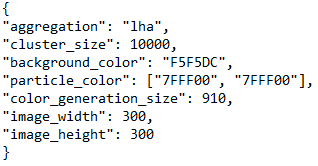
\includegraphics[height=3cm]{images/code-snippets/parameters.png} \\
\\
If correct parameters are set, you can run a shell script which in turn will run a single python file $\mathit{main.py}$ which reads the entered parameters and executes first the mathematical process which needs the mathematical imports and second the data creation of the calculated process which needs the systemic imports as described above. The created data will contain an image of the created cluster, a json file with the parameters saved for later lookup and another json file containing all calculated fractal dimension values and all particle coordinates for later lookup as well. \\
\\We will have a look now on what happens on the mathematical side. We will show code directly here to make things clearer. Note that in the original code here and there you will find comments or other irrelevant differences, which we leave away here. \\
\\The main executed python file $\mathit{main.py}$ looks like this:\\
\\
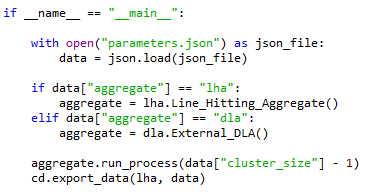
\includegraphics[height=4cm]{images/code-snippets/mainpy.png} \\
\\
Note again that you can also run an external DLA simulation but we do not claim that it is mathematically precise and therefore won't argument that in this paper. The parameters in $\mathit{parameters.json}$ are read and depending on which process (LHA or DLA) shall be simulated, the according object gets initiated and its $\mathit{run\_process}$ method gets executed. The init method of $\mathit{Line\_Hitting\_Aggregation}$ looks like the following:\\
\\
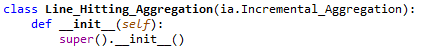
\includegraphics[height=2cm]{images/code-snippets/lhainit.png} \\
\\
We init the particle set $\mathit{particles}$ as a set containg $0$, init the boundary set which in every iteration of the process will contain all neighbours of all particles in the particle set, set the initial cluster radius to $0$ and init a list $\mathit{fractal\_dimension\_values}$ which will contain all values of fractal dimensions we calculate during the process, more on that later. We init this list to contain one value 1.5 to ensure that its length is equal to the amount of particles which is helpful for later calculation. We choose 1.5 since it is most neutral (since the fractal dimension lies in between 1 and 2 by \ref{notion} (\ref{trivialboundary})). Anyway this first value is not relevant and will not go into any calculation of later fractal dimension values. As neighbours we only consider the neighbour coordinates up, down, left and right as defined in \ref{zgraph}. \\
\\After initializing a $\mathit{Line\_Hitting\_Aggregation}$ object the code executes its $\mathit{run\_process}$ method, which looks like the following:
\\
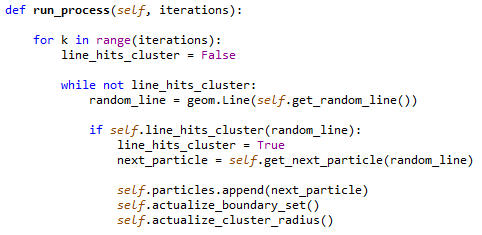
\includegraphics[height=5.3cm]{images/code-snippets/runprocess.png} \\
\\
This method will directly run a loop with $\mathit{data["cluster\_size"] - 1}$ iterations. In each iteration exactly one particle will be added to the particle set, so at the end we end up with exactly $\mathit{data["cluster\_size"]}$ particles since we started with one particle. \\
\\If we call $K$ the current cluster it is now important to understand again, how choosing random $K$-isotropic lines works. In \ref{choosekiso} we have argumented that a $K$-isotropic line can be realized by considering a circle $B$ which contains the current cluster $K$ and choose a $B$-isotropic line which intersects with the circle. If it happens that this line intersects with $K$, by \ref{circ} we know that we have realised a random $K$-isotropic line. The method $\mathit{get\_random\_line}$ \\
\\
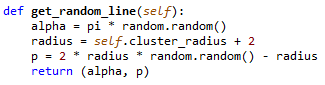
\includegraphics[height=1.8cm]{images/code-snippets/randomline.png} \\
\\
produces uniformly chosen line parameters, and using $\mathit{cluster\_radius + 2}$ here ensures that the line is hitting a surrounding circle $B$. The method $\mathit{random.random()}$ produces an uniformly chosen value in $[0,1)$. The fact that $\mathit{random.random()}$ cannot choose the value $1$ doesn't disturb the distribution of the line since $\{1\}$ is a zero set for the $2$-dimensional Lebesque-measure. By \ref{chi}, choosing these line parameters uniformly indeed realises a random $B$-isotropic line. \\
\\The method $\mathit{line\_hits\_cluster}$ \\
\\
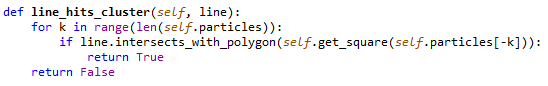
\includegraphics[height=1.8cm]{images/code-snippets/linehitscluster.png} \\
\\
bases on the method $\mathit{intersects\_with\_polygon}$ which evaluates whether a line intersects with a given polygon or not (the implemented geometry classes $\mathit{Line}$ and $\mathit{Polygon}$ you can find in the file $\mathit{geometry.py}$). Here the polygon is a square given by the method \\
\\
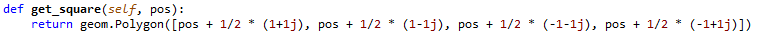
\includegraphics[height=0.8cm]{images/code-snippets/getsquare.png} \\
\\
which in total implements the definitions \ref{squares} and \ref{ghitA}. \\
\\If the condition is satisfied that a chosen line hits the cluster, we enter the if-condition and then choose the next particle with the method $\mathit{get\_next\_particle}$\\
\\
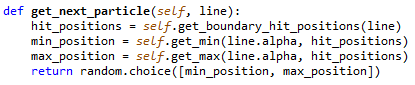
\includegraphics[height=1.8cm]{images/code-snippets/nextparticle.png} \\
\\
which first collects all particle squares which are hit by the line, calculates minimum and maximum and then chooses uniformly between minimum and maximum with $\mathit{random.choice}$. The methods $\mathit{get\_min}$ and $\mathit{get\_max}$ base on the method $\mathit{is\_lower}$\\
\\
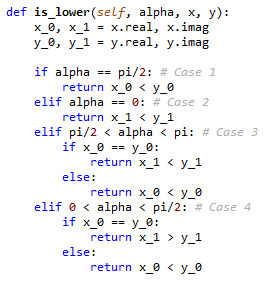
\includegraphics[height=6cm]{images/code-snippets/islower.png} \\
\\
which implements the total ordered relation on all squares which got hit by the line as defined in \ref{ghitA}. Minimum and maximum are then canonically calculated with respect to this relation. \\
\\After having realised the next particle, values like the particle set, the boundary set and the cluster radius get actualized and finally a new fractal dimension value is added to the fractal dimension values list. The method $\mathit{add\_fractal\_dimension\_value}$ \\
\\
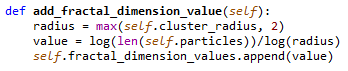
\includegraphics[height=1.5cm]{images/code-snippets/fractaldimension.png} \\
\\
devides the log of the current amount of particles in the cluster by the log of the current radius of the cluster as motivated by the definition \ref{notion} (\ref{fractaldimension}) of the discrete fractal dimension and adds this value to the $\mathit{fractal\_dimension\_values}$ list. Note that $\mathit{log}$ in python is the natural logarithm with base $e$. Also note that choosing the maximum of the cluster radius and $2$ only serves the purpose to avoid problems in the very beginning of the simulation when the cluster radius is $1$ and therefore creating division by zero in the subsequent division ($\log(1)=0$).\\
\\All in all this procedure should implement the distribution of the line hitting aggregation as mathematically defined. At the end its preciseness is depending on the preciseness of the distributions given by the python methods $\mathit{random.random}$ and $\mathit{random.choice}$, and machine calculation in general. Eventhough we do not claim to have implemented a mathematically precise simulation for external DLA, feel free to also try that one out and create beautiful pictures of the two incremental aggregations. 

\newpage

\section{Outlook}
In this paper we have looked at a general definition of incremental aggregations in $\Z^d$ and the notion of defining a fractal dimension for such discrete clusters. We have looked at two such incremental aggregations, the external diffusion limited aggregation and the line hitting aggregation, and have proved a rigorous result for the fractal dimension of external DLA.\\ 
CONTINUE\\
\\I hope that I have raised interest in the topic of incremental aggregations with this paper. I feel delighted to watch at the beautiful realizations of the aggregations and I hope the reader can feel similar looking at them and realizing images him- and herself. 

\newpage

\begin{thebibliography}{biblio}
\thispagestyle{empty}

\bibitem{wittensander}
T. A. Witten and L. M. Sander
\emph{Diffusion-limited aggregation}.
1983

\bibitem{stoch1}
Daniel Hug, Günter Last, Steffen Winter.
\emph{Stochastic Geometry, 	Lecture Notes (summer term 2020)}.
Institute of Technology, Karlsruhe, 2020

\bibitem{sackmann}
Franz Sackmann. 
\emph{Zufällige Geraden, Staatsexamensarbeit}.
University Karlsruhe (TH), Karlsruhe, 2007

\bibitem{lawler}
Gregory F. Lawler
\emph{Intersections of Random Walks}.
University of Chicago, 1996

\bibitem{henze}
Norbert Henze
\emph{Irrfahrten - Faszination der Random Walks}
Institute of Technology, Karlsruhe, 2018

\bibitem{fractalwinter}
Uta Freiberg, Ben Hambly, Michael Hinz and Steffen Winter
\emph{Fractal Geometry and Stochastics VI}
2020

\bibitem{magnetic}
J. Gonzalez-Gutierrez, J. L. Carrillo-Estrada and J. C. Ruiz-Suarez
\emph{Aggregation and dendritic growth in a magnetic granular system}
2013

\bibitem{hausdorff}
Egbert Brieskorn
\emph{Felix Hausdorff zum Gedächtnis, Band I, vieweg Verlag}
1996
page 160

\bibitem{markov}
Prof. Dr. Stefan Tappe
\emph{Markov-Ketten, lecture script summer semester 2018}
Abteilung für Mathematische Stochastik, Albert-Ludwigs-Universität Freiburg

\bibitem{ballistic}
D. Bensimon, B. Shraiman and S. Liang
\emph{On the ballistic model of aggregation}
Physics Letter, University of Chicago
1984

\bibitem{snowflake}
https://modernistcuisinegallery.com/


\end{thebibliography}

\newpage
  
\thispagestyle{empty}

\vspace*{8cm}


\section*{Erklärung}

Hiermit versichere ich, dass ich diese Arbeit selbständig verfasst und keine anderen als die angegebenen Quellen und Hilfsmittel benutzt, die wörtlich oder inhaltlich übernommenen Stellen als solche kenntlich gemacht und die Satzung des Karlsruher Instituts für Technologie zur Sicherung guter wissenschaftlicher Praxis in der jeweils gültigen Fassung beachtet habe. \\[2ex] 

\noindent
Karlsruhe, den 10. März 2020\\[5ex] 

\end{document}

